%%%%%%%%%%%%%%%%%%%%%%%%%%%%%%%%%%%%%%%%%%%%%%%%%%%%%%%%%%%%%%%%%%%%%%%%%%%%%%%
%
% Harvard ALM Thesis
%
% Author: Tony Allen (cyril0allen@gmail.com)
%
%%%%%%%%%%%%%%%%%%%%%%%%%%%%%%%%%%%%%%%%%%%%%%%%%%%%%%%%%%%%%%%%%%%%%%%%%%%%%%%

\documentclass[12pt]{article}
\usepackage[pdftex]{graphicx}
\usepackage{setspace,caption,url,tcolorbox,float,placeins,appendix,amsmath}
\doublespacing
\pagenumbering{gobble}

% Default margins are too wide all the way around. I reset them here
\usepackage[left=1.5in,right=1in,top=1in,bottom=1in,includefoot,nohead]{geometry}

%%%%%%%%%%%%%%%%%%%%%%%%%%%%%%%%%%%%%%%%%%%%%%%%%%%%%%%%%%%%%%%%%%%%%%%%%%%%%%%

\begin{document}
\begin{center}

  % Title  Two inches from the top of the page
  \vspace*{0.6in}
  Improving Data Placement Decisions for Heterogeneous Clustered File Systems

  % Full Name  2.5 inches below the first line of the Title
  \vspace{2.3in}
  Cyril Allen\\
  \vspace{1.8in}
  A Thesis in the Field of Information Technology\\
  for the Degree of Master of Liberal Arts in Extension Studies\\
  \vspace{.8in}
  Harvard University\\

  % Graduation Date, 2.5 inches from the bottom
  \vfill
  March 2018
  \vspace*{.5in}
\end{center}

\newpage
\null

\newpage

%%%%%%%%%%%%%%%%%%%%%%%%%%%%%%%%%%%%%%%%%%%%%%%%%%%%%%%%%%%%%%%%%%%%%%%%%%%%%%%
\section*{Abstract}
\thispagestyle{empty}

With the advent of cloud computing, datacenters are making use of distributed
applications more than ever. MapReduce is used to generate over 20 petabytes
of data per day using very large numbers of commodity servers
\cite{mapreduce}. Many companies use large scale clusters to perform various
computational tasks via the the open-source MapReduce implementation, Hadoop
\cite{hadoop}, or they can possess a virtualized datacenter allowing them to
migrate virtual machines between various machines for high-availability
reasons. As economics change for hardware, it is likely that a scalable cloud
will have the requirement to mix node types, which will lead to higher
performance and higher capacity nodes to be mixed with lower performance,
lower capacity nodes. This thesis presents an adaptive data placement method
in the Nutanix distributed file system which will remedy some common problems
found in many heterogeneous clustered file systems.

\clearpage
\newpage

%%%%%%%%%%%%%%%%%%%%%%%%%%%%%%%%%%%%%%%%%%%%%%%%%%%%%%%%%%%%%%%%%%%%%%%%%%%%%%%
\section*{Acknowledgements}
\thispagestyle{empty}

First off, I would like to thank my thesis director, Prof. Jamie Frankel. It
has been a truly amazing learning experience working with him.


I doubt I would be writing this document if it were not for my father, Dr.
Cyril Allen. Not only did he spark my initial interest in computing as a child,
he convinced me to pursue a graduate degree! Thanks, Dada.

Thanks are also due to my mother, Dr. Hengameh Allen-Schaal, for her
unconditional love and support. She has always been there for me when I needed
her, even when we began living in different states. I could not have done any
of this without her.

Monique Fahmy

% Nutanix/Pete, for hardware and resources

% Harvard? eh..

\clearpage
\newpage

%%%%%%%%%%%%%%%%%%%%%%%%%%%%%%%%%%%%%%%%%%%%%%%%%%%%%%%%%%%%%%%%%%%%%%%%%%%%%%%
\pagenumbering{roman}

\tableofcontents
\newpage

\listoffigures
\newpage

\listoftables
\newpage

\pagenumbering{arabic}

%%%%%%%%%%%%%%%%%%%%%%%%%%%%%%%%%%%%%%%%%%%%%%%%%%%%%%%%%%%%%%%%%%%%%%%%%%%%%%%
\newpage
\FloatBarrier
\section{Introduction}

  The work in this thesis was performed in the context of a distributed file
  system designed by Nutanix for enterprise clusters. Given that a write
  operation that results in the creation of new data in this file system is not
  complete until all replicas of the data are written to disk, a write's
  performance is at the mercy of the slowest disk in the set chosen to host
  replicas and all entities those disks are dependent on. These entities could
  include variables such as the server's average CPU utilization and the number
  of operations already in flight on a chosen disk. To mitigate the negative
  impact these variables could have on a write, the file system should take
  into account how these variables will affect a disk's performance before
  choosing to target it for a write operation. This results in biasing toward
  disks that will give better performance overall.

  \begin{figure}[htbp]
    \centering
    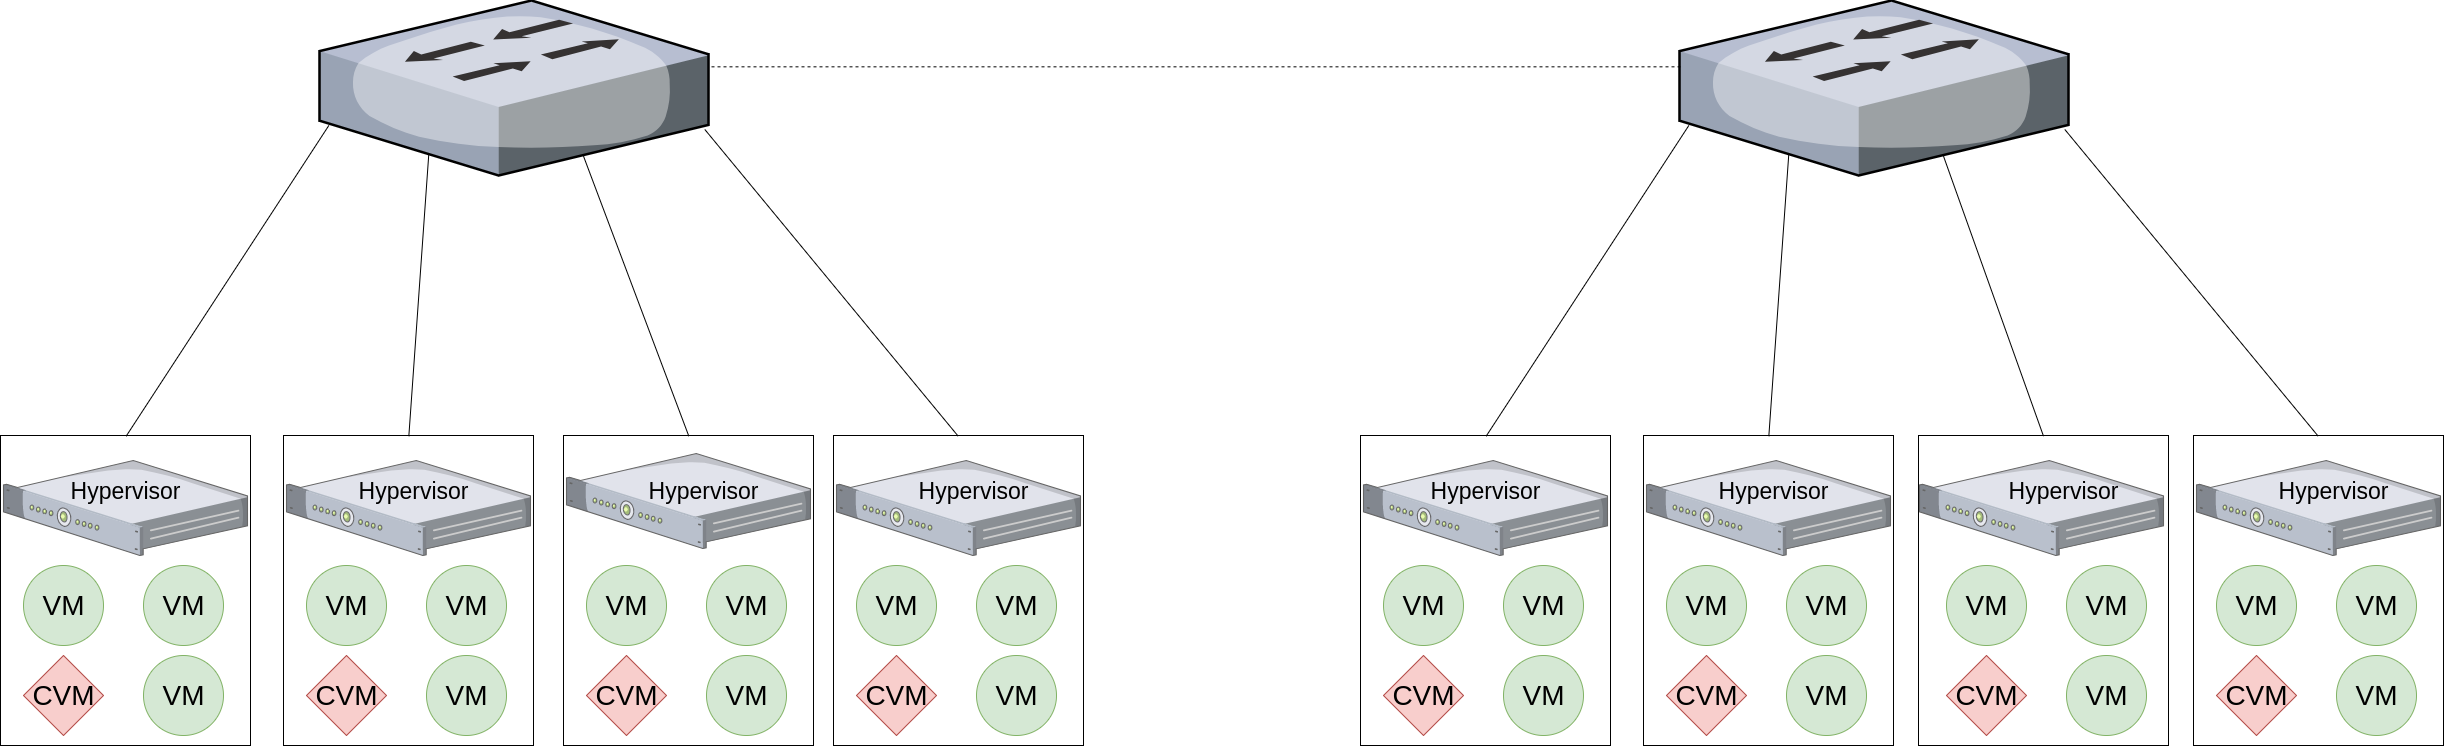
\includegraphics[scale=0.19]{images/network_diagram.png} 
    \caption{Testing size.}
    \label{fig:adsf-network}
  \end{figure}

  \subsection{Nutanix and the Acropolis Base System} \label{sssec:abs}

    \subsubsection{Architecture}

    A Nutanix cluster is facilitated by a clustering of controller virtual
    machines (CVMs) which reside, one per node, on each server in the cluster
    as shown in Figure \ref{fig:adsf-architecture}. CVMs work together to form
    a distributed system that provides an NFS (for VMWare's ESXi
    \cite{esxi2008}), SMB (for Microsoft's Hyper-V \cite{hyperv2009}), or iSCSI
    (for Nutanix's AHV \cite{bible}) interface to each hypervisor that they
    reside on. For example, the interface provided by the CVMs to VMware's ESXi
    hypervisor will be interfaced as a storage target, or in ESXi terminology,
    a datastore. The virtual machines' virtual disk files will reside on the
    Nutanix datastore and be accessed via NFS through the CVM sharing a host
    with the other hosted VMs.

    Users of a Nutanix cluster will typically have virtual machines (VMs)
    hosted by one of the hypervisors previously mentioned. These VMs will have
    their storage requests forwarded to the local CVM hosted on the same node,
    or another CVM in the cluster in the event that the local CVM is down. This
    fault tolerance is one of the advantages to using a clustered file system
    such as Nutanix as opposed to a monolithic storage array.
    
    \begin{figure}[htbp]
      \centering
      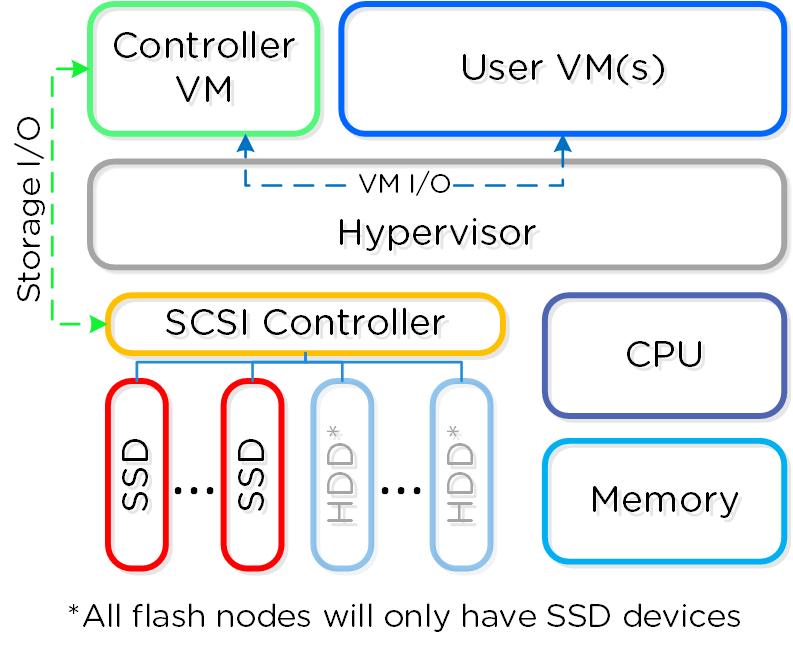
\includegraphics[scale=1.0]{images/converged_platform.png} 
      \caption{Nutanix node architecture diagram from the Nutanix
               Bible\cite{bible}.}
      \label{fig:adsf-architecture}
    \end{figure}

    The CVMs expose some number of block devices, known as vDisks, that are
    used by the VMs hosted by the hypervisor. Within each CVM exists an
    ecosystem of processes responsible for the services provided by the Nutanix
    cluster. The work in this thesis is scoped specifically to the process that
    is directly responsible for disk I/O in the CVM ecosystem, Stargate.

    \subsubsection{Stargate} \label{section-stargate}

    The Stargate process is responsible for all data management and I/O
    operations. The messages sent via NFS/SMB/iSCSI from the hypervisor to the
    CVM are consumed and acted upon by Stargate. All file allocations and data
    replica placement decisions are made by this process.

    As the Stargate process facilitates read/write I/O to physical disks, it
    gathers statistics for each disk such as the number of operations currently
    in flight on the disk (queue length), how much data in bytes currently
    resides on the disk, and the average time to complete an operation on the
    disk. These statistics are only gathered on the local disks; however, they
    are then stored in a distributed database via another service, Arithmos.
    Along with the statistics gathered by every other Stargate in the cluster,
    these disk statistics stored in the database and are pulled periodically
    and are then used to make decisions on whether a disk has enough space
    available to make it a write target. The work in this thesis uses other
    available statistics to make better placement decisions when performing
    writes.

    \subsubsection{Cassandra}

    Cassandra stores and manages all cluster metadata in a distributed manner.
    It is also the distributed database used by Arithmos to store cluster
    statistics. The version of Cassandra running in NDFS is a heavily modified
    Apache Cassandra \cite{cassandra}. One of the main differences between
    Nutanix Cassandra and Apache Cassandra is that Nutanix has implemented
    strict consistency via Lamport's Paxos \cite{paxos2005} protocol.

    % TODO: elaborate on Paxos?

    \subsubsection{The Extent Store}

    The Extent Store is a sub-component of Stargate that serves as the
    persistent bulk storage. Data stored within the Extent Store are referred
    to as extent groups (also abbreviated as egroups), or 4MB pieces of
    physically contiguous data. An extent group is replicated a number of
    times dependent on the cluster replication factor and each replica is
    placed on a different CVM except for a single replica that resides on the
    local node. The current replica selection algorithm will be explained in
    further detail in section \ref{sec:replica-selection}.

    \subsubsection{Storage Tiering and Data Replication}

    Data in the system is physically stored on disks of varying type. Within a
    given cluster, one can find NVMe, PCIe SSD, SATA SSD, and HDD drive types.
    These disks are separated into groups of drives with similar performance
    characteristics, referred to as storage tiers. For example, PCIe SSDs and
    SATA SSDs might belong together in the same storage tier, but hard drives
    would not be included due to their relatively poor random access
    performance. Extent groups and their replicas are created on a particular
    storage tier, but may be migrated between tiers depending on data access
    patterns.

    Data replicas for each extent group are written on separate fault domains
    on the same tier to ensure that in the event a failure occurs and a
    replica becomes unavailable, that piece of data can still be accessed. An
    example of a fault domain can be a node (single CVM) or a block (a rackable
    unit of hardware containing multiple nodes). 

    \subsubsection{Replica Selection} \label{sec:replica-selection}

    Stargate is inherently limited in its choices of disk to service reads
    since it must select a disk that contains the desired data. If the data is
    on a local disk, this disk is always selected to avoid the unnecessary
    overhead of data traversal over the network when selecting a remote disk.
    However, when selecting disks to service writes, Stargate must decide
    whether to perform an in-place overwrite for writes over existing ranges of
    data or whether to generate new data. In-place overwrites are similar to
    reads in that the choice of target disk is limited by where the relevant
    data resides. When enabling a common data reduction feature such as data
    deduplication, in-place overwrites are not performed since the metadata for
    multiple logical ranges of data point to the same physical data. In the
    case of overwrites of deduplicated data and all scenarios where data is
    being created for the first time, Stargate has the freedom to choose any
    disk in the cluster.

    When a Stargate write operation wants to select disks for data placement
    upon entrance into the Extent Store, it is done on a per-tier basis. The
    interface for a replica selection function call, DetermineNewReplicas,
    takes the following arguments:

    \begin{table}[htbp]
      \caption{Argument descriptions for DetermineNewReplicas.}
      \begin{tabular}{ | p{0.4\linewidth} | p{0.6\linewidth} | }
        \hline
        \textbf{Argument Name} & \textbf{Description} \\ \hline
        \verb|replica_vec| & A \texttt{std::vector} that is populated with the selected
                             disk IDs. The number of selections made is the
                             size of this vector. \\ \hline

        \verb|storage_tier| & The name of the storage tier (set of disks) to
                              select for data placement. \\ \hline
 
        \verb|storage_pool_vec| & The collection of all disks in the cluster.  \\ \hline

        \verb|preferred_node_vec| & Nodes Stargate prefers to choose disks from. This
                                    means it will consider disks from these
                                    nodes first and only consider other disks
                                    if the ones belonging to these nodes are
                                    not suitable. \\ \hline

        \verb|predicate_func| & A function that accepts a disk ID and returns a
                                boolean. If this function returns false
                                for any disk ID, it is not considered for
                                selection. \\ \hline

        \verb|exclude_replica_vec| & Disk IDs that will be excluded from
                                     selection. \\ \hline

        \verb|exclude_node_vec| & Node IDs whose disks will be excluded from
                                  selection. \\ \hline

        \verb|exclude_rackable_unit_vec| & Rack IDs whose disks will be
                                           excluded from selection. \\ \hline

        \hline
      \end{tabular}
    \end{table}

    Upon calling DetermineNewReplicas, Stargate first attempts to select replicas from
    the preferred nodes. This involves finding the set of disks that belong to
    each node on the specified tier, shuffling the disks, and sequentially
    evaluating each disk until a suitable one is found (the evaluation step).
    If a suitable disk is not found on a preferred node, all other disks
    belonging to the specified tier are shuffled and considered sequentially
    until enough disks are found to satisfy the requirement set by replica\_vec.

    A suitable disk is one that:

    \begin{tcolorbox}
    \begin{enumerate}
      \item Contains enough space to accept new data. This is less than 95\% by
            default for Nutanix clusters.  \item Returns "true" when evaluated by the
            predicate\_func.
      \item Is not included in the exclude\_replic\_vec, exclude\_node\_vec,
            and exclude\_rackable\_unit\_vec.
    \end{enumerate}
    \end{tcolorbox}

    If a disk does not meet the criteria above, Stargate simply continues searching
    the shuffled set of disks belonging to the specified tier. If a disk is
    found to be suitable, Stargate must add the disk to the replic\_vec and add
    the node that the disk belongs to in the exclude\_nod\_vec. This prevents
    it from considering other disks on that node to maintain a node fault
    tolerance guaranteed by the cluster's replication factor.

  \subsection{Motivation}

  The current replica disk selection logic in Stargate uses does not take into
  account a number of variables such as disparities in tier size, CPU power,
  workloads, and disk health among other things. There are several scenarios,
  both pathological and daily occurences, where a more robust replica placement
  heuristic is required. The work in this thesis will focus on two orthogonal
  cases described in the next section.

    \subsubsection{Interfering Workloads}

    \begin{figure}[htbp]
      \centering
      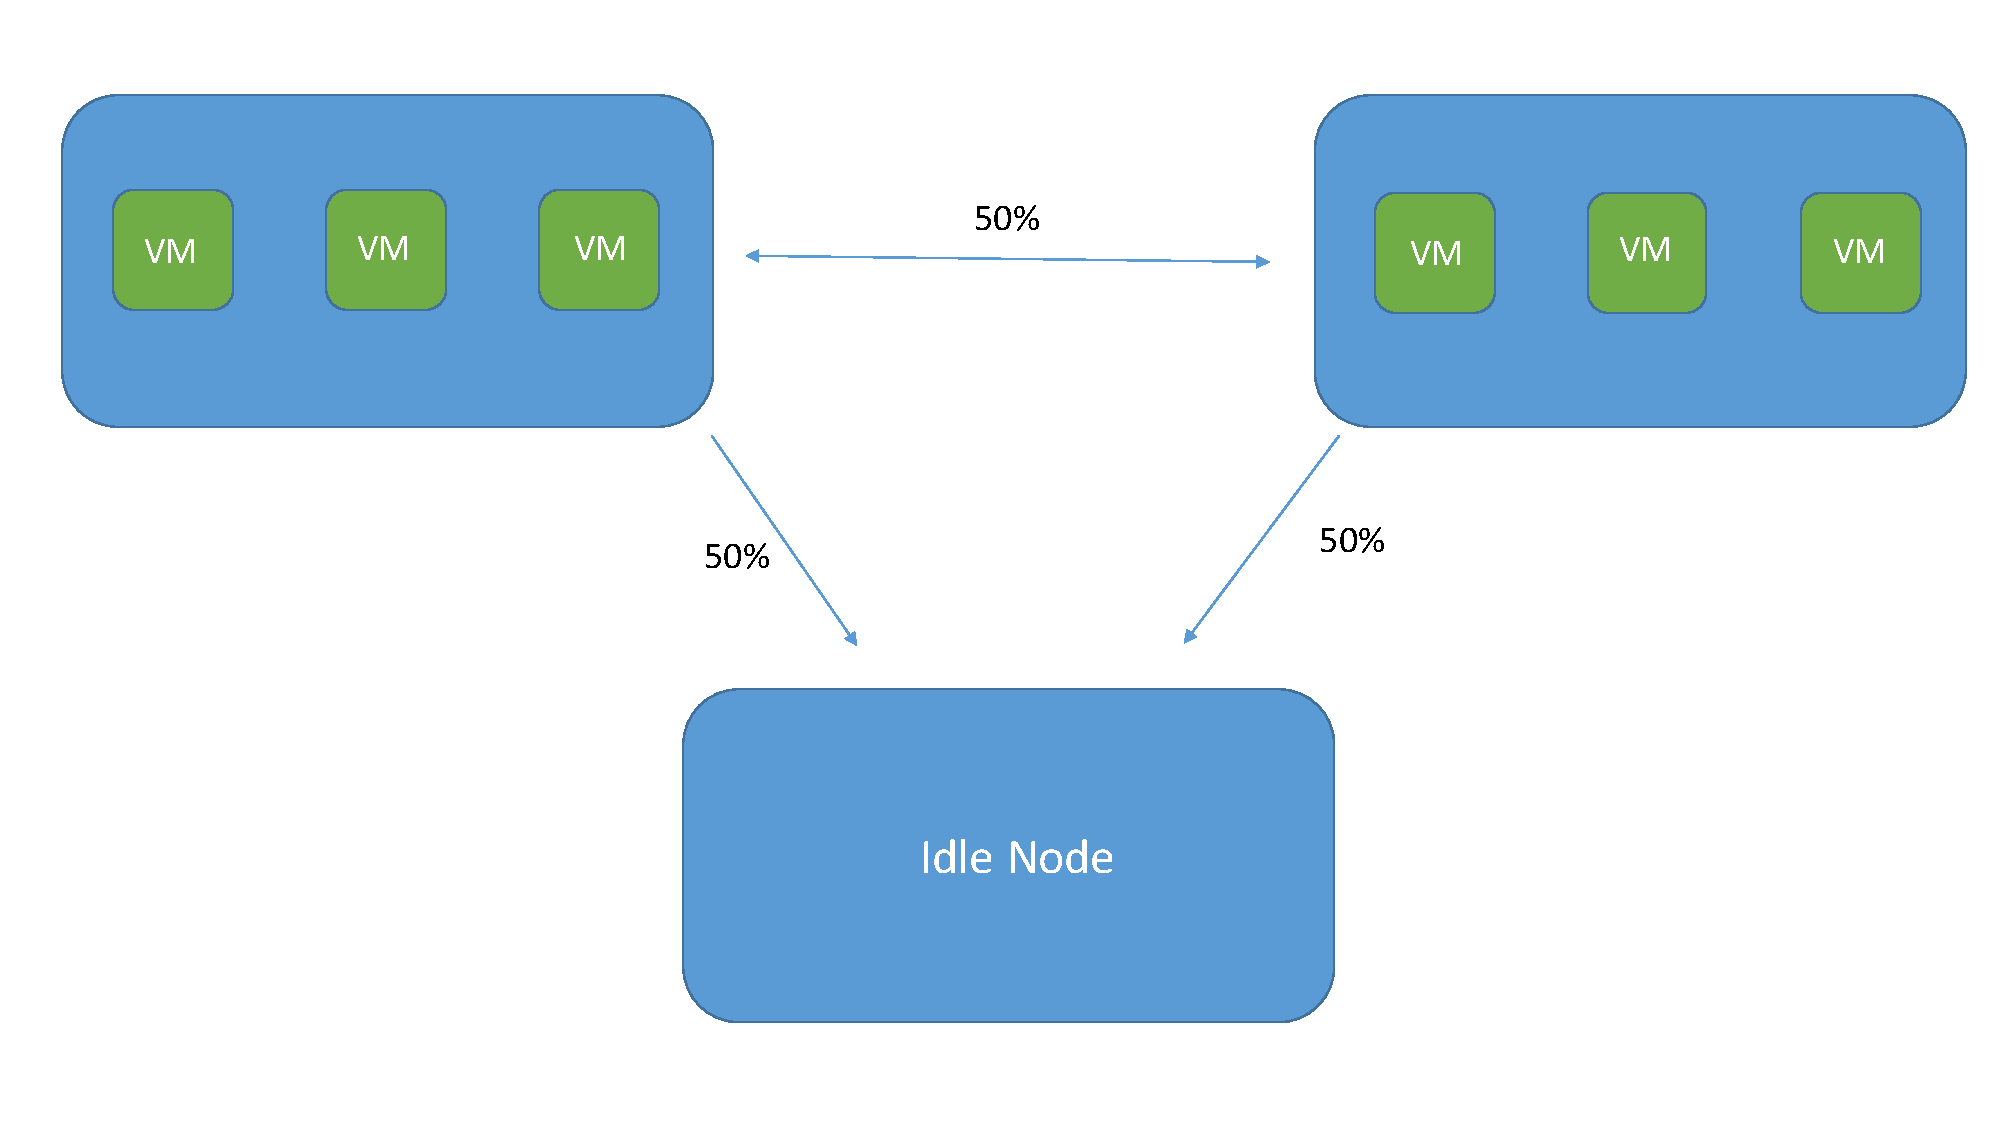
\includegraphics[scale=0.45]{images/homogeneous_workload_disparity.pdf} 
      \caption{A cluster with identical nodes running a heterogeneous workload.}
      \label{fig:workload_disparity}
    \end{figure}

    As shown in Figure \ref{fig:workload_disparity}, interfering workloads can
    take the form of a homogeneous cluster of 3 servers in a full mesh network
    (also referred to as a 3 node cluster) with only 2 nodes hosting active
    workloads. In the current random selection scheme used by Nutanix
    clusters, writes in this example are equally likely to place their replica
    on the remote node with an active workload as they would be to place it on
    the remote node that is idle.  This can impact performance on both the
    local and remote workloads as secondary writes will be slower on nodes
    whose resources are being utilized by their primary workloads. A data replica
    placement scheme is needed that adapts its behavior based on how less busy
    the target nodes are. This would result in a bias towards nodes that are
    more idle.

    \subsubsection{Nodes with Tier Size Disparities}

    A cluster containing nodes with a tier size disparity are susceptible to a
    large skew in space utilization on the node, even if the workload on each
    node is identical. This can be illustrated via Figure
    \ref{fig:tier_size_disparity} which shows a 3-node heterogeneous cluster
    with 2 high-capacity nodes and a single low-capacity node.  Suppose these
    high-capacity nodes have 500GB of SSD tier, 6TB of HDD tier and the single
    weak node has only 128GB of SSD tier and 1TB of HDD tier. If 3 simultaneous
    workloads were to generate data such that the working sets of these
    workloads are 50\% of the local SSD tier, the weaker node is at a
    significant disadvantage. Given the replica selection algorithm in Nutanix
    cluster versions prior to 5.0, one can expect 500GB of replica traffic to
    flood the weak node and fill up its SSD tier well before the workload is
    able to write its data to the local disks.  Since this results in an
    inability for the workload on the smaller node to place its primary
    replicas locally and forces the workload to rely on remote CVMs, latency is
    increased due to the network traversal to reach the remote nodes. An
    adaptive replica placement heuristic would mitigate this issue by taking
    disk usages into consideration during the placement of secondary replicas
    and bias placement of secondary replicas toward the nodes with more free
    capacity.

    \begin{figure}[htbp]
      \centering
      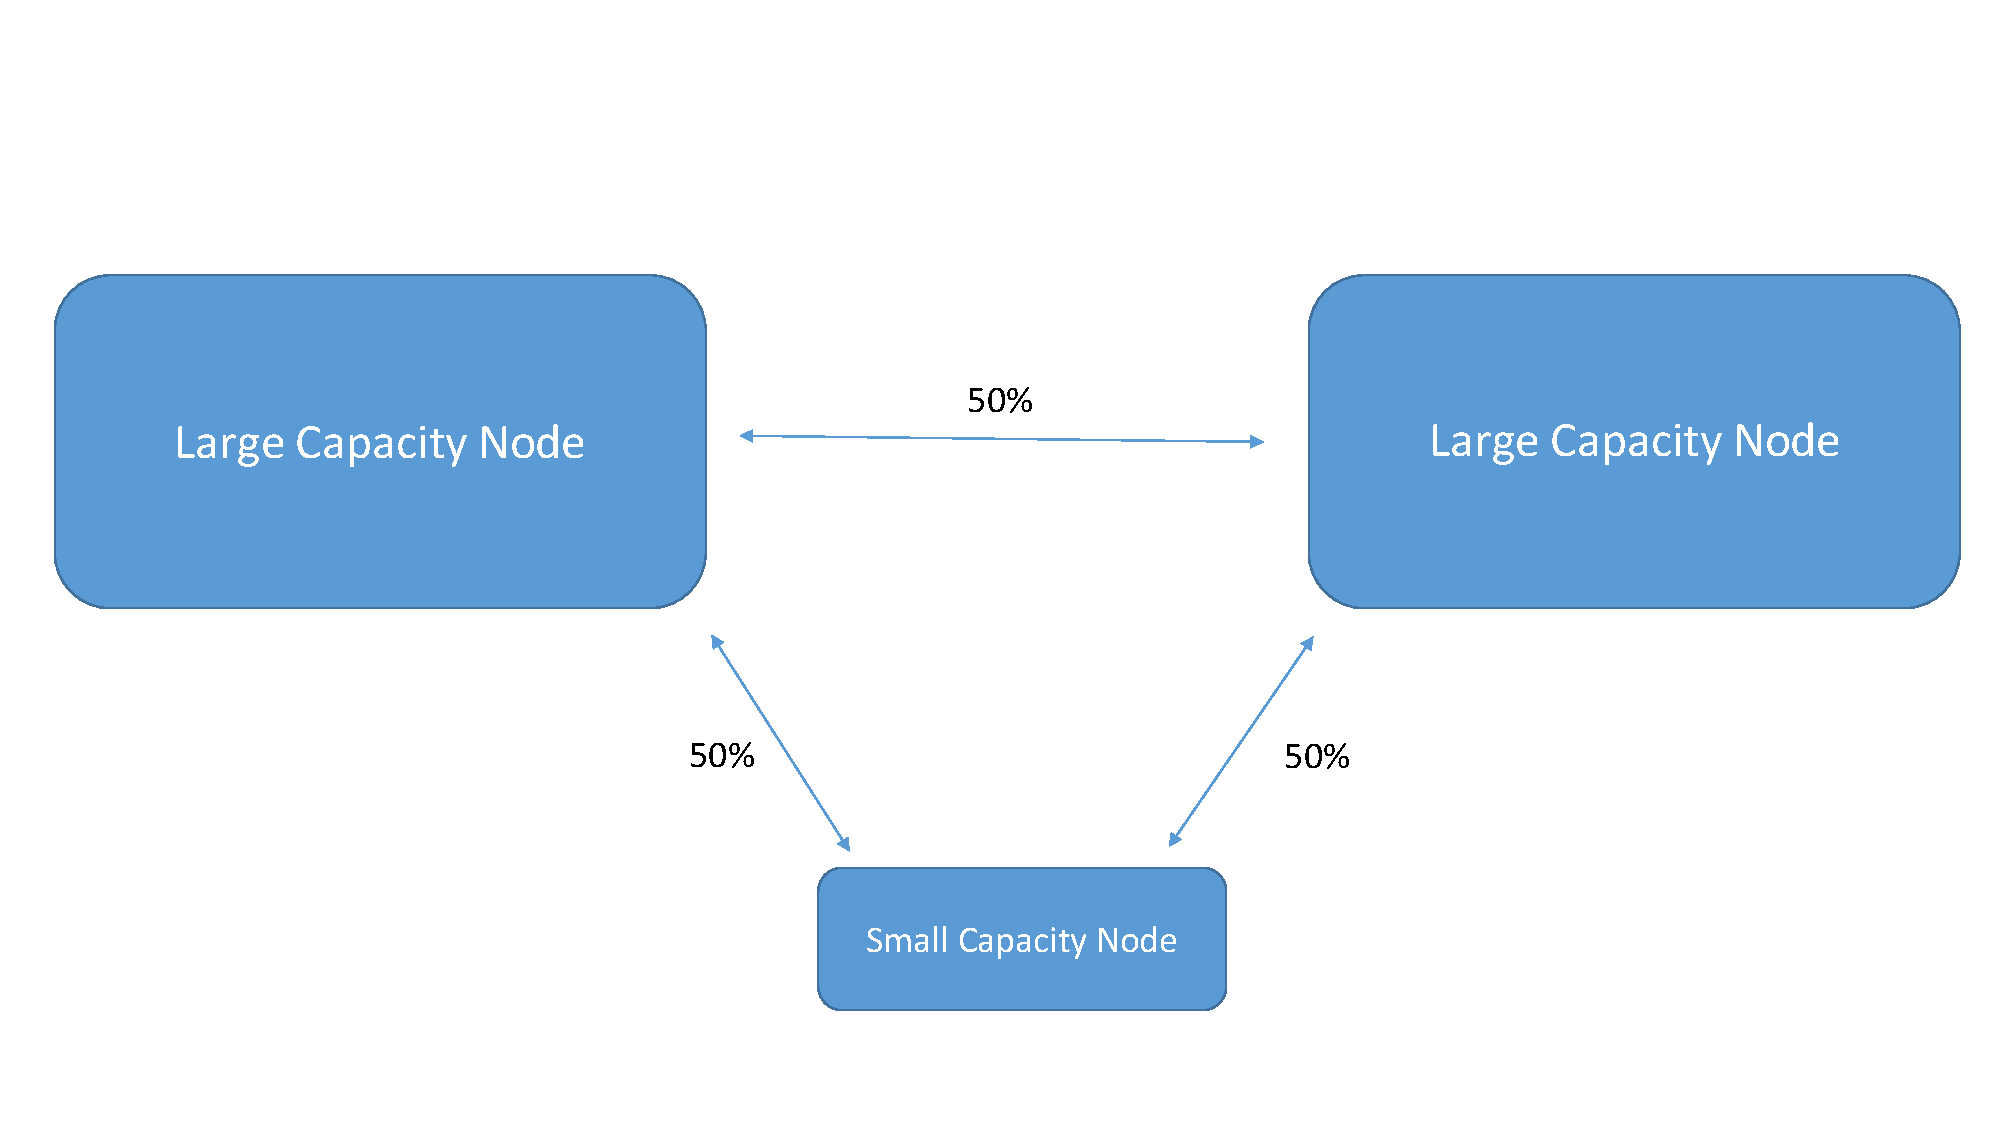
\includegraphics[scale=0.45]{images/homogeneous_tier_disparity.pdf} 
      \caption{A cluster with nodes of varying resource capacity.}
      \label{fig:tier_size_disparity}
    \end{figure}

    To create a context for the work in this thesis, it's necessary to delve
    deeper into what a Nutanix cluster is and give a brief overview of the
    I/O path. Section \ref{sssec:abs} will be devoted to this overview.

%%%%%%%%%%%%%%%%%%%%%%%%%%%%%%%%%%%%%%%%%%%%%%%%%%%%%%%%%%%%%%%%%%%%%%%%%%%%%%%
\newpage
\FloatBarrier
\section{Prior Work}

  \subsection{Clustered Storage Systems}

  Among the contemporary distributed storage systems, Apache's Hadoop
  Distributed File System (HDFS) \cite{hadoop} is one of the most well known.
  HDFS is an open source distributed file system written as a userspace library
  in Java that is used by Hadoop clusters for storing large volumes of data. An
  HDFS cluster is comprised of a single NameNode and multiple DataNodes which
  respectively manage cluster metadata and store the data. HDFS stores files as
  a sequence of same-size 128MB blocks that are replicated across DataNodes to
  provide fault tolerance in the event of node failures. Decisions regarding
  the replication and placement of blocks of data are made by the NameNode.
  Since large HDFS clusters will span multiple racks, replica placement within
  HDFS is made in a rack-aware manner to improve data reliability and network
  utilization.

  While HDFS is an open source distributed file system that is part of the
  greater Apache Hadoop ecosystem, the Google File System (GFS) \cite{gfs} is a
  proprietary distributed file system developed by Google that inspired HDFS. A
  GFS cluster is comprised of a single Master node and multiple Chunkservers
  that store 64MB "chunks," or blocks, of data. Each file in the GFS is divided
  into the 64MB chunks and each chunk is replicated by the Chunkservers
  multiple times throughout the GFS cluster. Master nodes store the metadata
  associated with the chunks such as chunk location or which processes are
  operating on a chunk.

  \subsection{Data Placement Schemes in Clustered Storage Systems}

  Xie et. al. \cite{xie2010} showed that data placement schemes based on the
  computing capacities of nodes in the HDFS significantly improved workload
  performance. These computing capacities are determined for each node in the
  cluster by profiling a target application leveraging the HDFS. Their
  MapReduced \texttt{wordcount} and \texttt{grep} results showed up to a 33.1\%
  reduction in response time. Similarly, Perez et. al. \cite{perez2003} used
  adaptive data placement featurers that make use of data regarding the
  available free space in their Expand parallel file system design.  Though
  effective in their given contexts, the main drawback to this approach is that
  it assumes the specific application is working without interference and does
  not account for other workloads on the system.

  One adaptive data placement approach that can account for other workloads on
  the system was introduced by Jin et. al. \cite{adapt2012} in their work on
  ADAPT . The study predicts how failure-prone a node in a MapReduce cluster is
  and advises their availability-aware data placement algorithm to avoid those
  nodes. This proves useful for performance by avoiding faulty nodes that could
  fail mid-task and cause data transfers and re-calculation of data.

  Work by Suresh et. al. \cite{suresh2015} approaches adaptive replica
  selection in much the same way as this thesis, though their work was
  mainly focused on decreasing tail latencies for Apache Cassandra
  \cite{cassandra} reads. Their load balancing algorithm, C3, incorporates the
  concept of a value calculated from request feedback from their servers. The
  value then guides decisions made regarding which servers to select for future
  requests.  In addition to the ranking function in C3, they implemented a
  distributed rate control mechanism to prevent scenarios where many individual
  clients can bombard a single highly desirable server with requests. Many of
  the same problems that the work in this thesis seeks to remedy are addressed
  by the C3 algorithm, such as the reduction of I/O latency. However, the C3
  algorithm is not a feasible solution when it comes to reducing each Nutanix
  node's disk utilzation skew relative to the other nodes in the cluster.

  The C3 algorithm takes into account the request queue length of certain
  servers similar to the way I will use disk queue lengths. In addition Suresh
  et. al. factor in the service latencies of each server so that they may
  consider a different ideal queue length for each server. With this approach,
  longer service times will warrant a lower queue length and vice versa. This
  is beneficial for scenarios where there are multiple underlying storage
  technologies such as NVMe drives, SSDs, and HDDs under consideration, but the
  Nutanix file system's architecture does not allow for multiple replicas to
  span storage tiers. This forces the ideal queue lengths for each selection
  pool to be the same. Therefore, this thesis does not incorporate service
  latencies in the fitness value calculations discussed in section
  \ref{section-fitness}.

  Herding of requests to a single highly suitable server is a problem that
  arises in any replica ranking algorithm. C3 mitigates this issue by rate
  limiting client requests to each server via a decentralized calculation using
  a configured time interval and local sending rate information. I've opted to
  use a simpler probabilistic spreading of client requests via selecting remote
  nodes using weighted random selection based on the calculated fitness values.
  This fitness value approach was inspired by Cisco's Enhanced Interior Gateway
  Routing Protocol (EIGRP) \cite{eigrp} and its composite routing metric
  calculations discussed further in section \ref{eigrp-motivation}.

  \subsection{Non-clustered Data Replication via RAID}

  So far, I have only discussed distributed file systems and data replica
  placement schemes in a clustered/distributed context. It is worth noting
  that not all storage replication occurs across a network partition. For
  example, it is common to see Redundant Arrays of Inexpensive Disks (RAID)
  \cite{raid} \cite{raid2} used on servers to increase performance or to
  protect data written to the disks in the event of a drive failure.

  \begin{table}[htbp]
    \caption{Common RAID levels and their descriptions.}
    \label{tbl:raid-levels}
    \begin{center}
    \begin{tabular}{ | l | l | }
      \hline
      \textbf{RAID Level} & \textbf{Description} \\ \hline
      RAID 0 & Disk striping with no replication. \\ \hline
      RAID 1 & Disk mirroring. \\ \hline
      RAID 5 & Block-level striping with distributed parity. \\ \hline
      RAID 6 & Block-level striping with doubly distributed parity. \\ \hline
      \hline
    \end{tabular}
    \end{center}
  \end{table}

  RAID combines multiple physical disks into a single logical disk that is then
  presented to the operating system as a single device. The exact data
  replication scheme that dictates the way data is distributed across the
  drives is known as the RAID level. Table \ref{tbl:raid-levels} shows some of
  the standard RAID levels.

  \subsection{EIGRP and the Inspiration for Fitness Values}
  \label{eigrp-motivation}

  EIGRP \cite{eigrp} is Cisco's proprietary routing protocol and enhancement to
  their Interior Gateway Routing Protocol (IGRP). In EIGRP, each router
  keeps information about its adjacent neighbors containing the address and
  interface of the connected neighbor. This information is needed because of
  the Topology Table (also referred to as the Distance Table) which contains
  the distance, bundled with an associated metric, to all destinations
  advertised by the adjacent neighbors. The metrics across all paths to the
  destination are stored in the distance table and are used to calculate the
  minimum cost path to a particular destination.

  \begin{equation}
    Term_{1} = K_{1} * \frac{K_{2} * Bandwidth}{Bandwidth + 256 - Load} + K_{3} * Delay
  \end{equation}

  \begin{equation} \label{eigrp-metric-eq}
    Metric = 256 * Term_{1} * \frac{K_{5}}{K_{4} + Reliability}
  \end{equation}

  Equation \ref{eigrp-metric-eq} shows the formula used by Cisco routers to
  calculate the distance metric. Note that as bandwidth increases, the metric
  is increased; however, as load increases on the links the metric decreases.
  There are constant values, also known as K-values, that allow network
  engineers to modify the behavior of the network based on their preferences.
  This idea of taking desirable traits and using them to calculate a metric, or
  desirability value, can be applied to the problem of choosing the best disk
  for data replica placement. This concept will be explored further in the
  following sections within the context of the Nutanix distributed file system.

%%%%%%%%%%%%%%%%%%%%%%%%%%%%%%%%%%%%%%%%%%%%%%%%%%%%%%%%%%%%%%%%%%%%%%%%%%%%%%%

\newpage
\FloatBarrier
\section{Implementation}

  \subsection{Fitness Values and Functions} \label{section-fitness}

  To calculate a value to represent the desirability of a disk for replica
  placement, a function, $f_{fitness}$, is defined. $f_{fitness}$ takes as its
  argument, some number of variables that can affect disk performance and
  returns a positive number henceforth referred to as a fitness value.
  
  A low fitness value indicates a poor placement candidacy for a disk and a
  high fitness value will indicate a highly desirable disk for replica
  placement. In this work, I evaluate two fitness functions that are
  comprised of terms that utilize a disk's average queue length over some
  stretch of time, $t_{q}$, and a disk's percentage utilization, $t_{u}$.

  \begin{equation}
    t_{q} = 1 - \frac{q}{q_{ceil}}
  \end{equation}

  The variable $q_{ceiling}$ holds the maximum observed queue length.
  Increasing $t_{q}$ beyond $q_{ceiling}$ does not contribute to the fitness
  value. This ensures that as the queue length grows, $t_{q}$ approaches zero. 

  \begin{equation}
    t_{u} = \frac{1}{a^{u}}
  \end{equation}

  The variable $u$ represents disk utilization percentage and $a$ is an
  aggression variable used to control the exponential decay of $t_{u}$. The
  larger $a$ is, the more aggressively $t_{u}$ will decay as $u$ increases. An
  aggressive decay results in more preference given to less utilized disks when
  compared with disks that are slightly more utilized.

  These terms are used in two different fitness functions evaluated in this
  document:

  \begin{equation} \label{eqn:additive-fitness}
    f_{add} = t_{u} + t_{q}
  \end{equation}

  \begin{equation} \label{eqn:multiplicative-fitness}
    f_{mult} = t_{u}t_{q}
  \end{equation}


  \subsection{Stargate Disk Stats Collection}

  Prior to this work, Stargate's periodic disk stats collection was limited to
  caching solely disk usage stats for all disks in the cluster. This has been
  expanded to now include disk performance stats for use in disk fitness
  values.

  Stargate maintains a mapping, henceforth referred to as the $disk\_map\_$,
  from cluster disk ID to a disk state structure. The $disk\_map\_$'s state
  structure contains disk usage and performance information that has been
  published to Arithmos by other Stargates in the cluster. Upon gathering fresh
  stats from Arithmos, the information is used to create a disk fitness value
  for each disk in the cluster.

  \subsection{Weighted Random Selection Algorithms}

  After a weight is calculated for a disk in the cluster that will store a
  replica, the \texttt{WeightedVector} class' \texttt{Sample()} calls will
  perform a weighted random selection on the set of potential candidate disks.
  To determine the best method of weighted random selection for Stargate's
  \texttt{WeightedVector} class, an exploration of various weighted random
  selection algorithms was necessary.  Since the file system only supports
  replication factors of 2 or 3, the investigation was limited to algorithms
  that allow for a weighted $\binom{N}{K}$, where $K$ is the data replication
  factor.

    \subsubsection{Scalability Simulation Methodology}
     To test the scalability of the weighted random selection algorithms
     evaluated in the next section, a single-threaded Python \cite{python}
     script was written to to evaluate the change in run time as sample sets
     increase. Each algorithm's mean running time is calculated for multiple
     sample sets. Code for the simulations is as follows:

     \singlespace
     \begin{tcolorbox}
     \begin{verbatim}
       def gen_runtimes(selection_func, iteration_count):
         runtimes = []
         std_devs = []
         # For each pool size.
         for pool_size in num_disks_for_tests:
             print("Measuring with pool size " + str(pool_size))
             runtime_list = []
             # Make a list of pool_size random numbers between 1 and 10.
             lst = pool_size * [1]
             # Time selections and get the average runimes.
             for it in range(iteration_count):
                 start_time = time.time()
                 selection_func(lst)
                 elapsed_time = time.time() - start_time
                 runtime_list.append(elapsed_time)
             avg_runtime = np.average(runtime_list)
             std_dev = np.std(runtime_list)
             runtimes.append(avg_runtime)
             std_devs.append(std_dev)
         return runtimes, std_devs
     \end{verbatim}
     \end{tcolorbox}
     \doublespace
        
    Object weights are constant throughout the simulation, so selection schemes
    that require some amount of preprocessing (such as the top T\% calculation
    for truncation selection) perform their preprocessing steps for each
    weighted random selection. This gives information about the worst-case
    run time behavior for each algorithm in comparison with the worst case
    runtime of the others.

    \subsubsection{Herding Behavior Evaluation Methodology}
    Herding behaviors can be seen in some weighted random selection
    algorithms when the weights of a subset of objects in the sampling pool
    cause a disproportionate amount of selections to target those objects. In
    the case of replica disk selections in a Nutanix cluster, this can cause
    too many operations to target an especially suitable disk, resulting in
    poor performance. It is possible to simulate an exaggerated scenario in
    which the susceptibility to herding behavior can be observed by having a
    single object with a weight that is multiple orders of magnitude heavier
    than the next highest object in the sampling set. It is also necessary to
    observe any herding behavior for a sampling set with low weight skew. This
    section describes the simulation methodology for each.

    High-skew sampling sets of 11 objects were generated such that the array
    index of the first 10 objects was assigned as the object weight, and the
    last object was given a weight of 1000. This creates an extremely large
    skew in weights and makes the high-weight object a target for herding
    behavior. Given this sampling set, weighted random selections were
    performed and a histogram was kept that tracked the number of selections
    for each object. $10^3$, $10^4$, and $10^5$ iterations were performed to
    observe any changes in herding behavior at larger time scales. In addition
    to the high-skew sampling sets, low-skew sets of 100 objects were also
    simulated.  These low-skew sets were identical to the high-skew sets,
    except there was not a single object with an exaggerated weight of 1000.
    All element weights were their array indices.

    \subsubsection{Stochastic Universal Sampling (SUS) Simulations}
    SUS is another sampling technique first introduced by Baker in 1987
    \cite{baker1987}. The algorithm can be understood as follows: On a
    standard roulette wheel there's a single pointer that indicates the winner.
    The roulette wheel's "bins" can all be the same size which would indicate a
    uniform probability of selecting any bin and could also be unevenly sized
    which would indicate a weighted probability. SUS uses this same concept
    except allows for N evenly spaced pointers corresponding to the selection
    of N items. Key things to note are that the set, or "bins" in my roulette
    analogy, must be shuffled prior to selection. Also, there is a minimum
    spacing allowed for the pointers to prevent selection of the same bin.

    \begin{figure}[htbp]
      \centering
      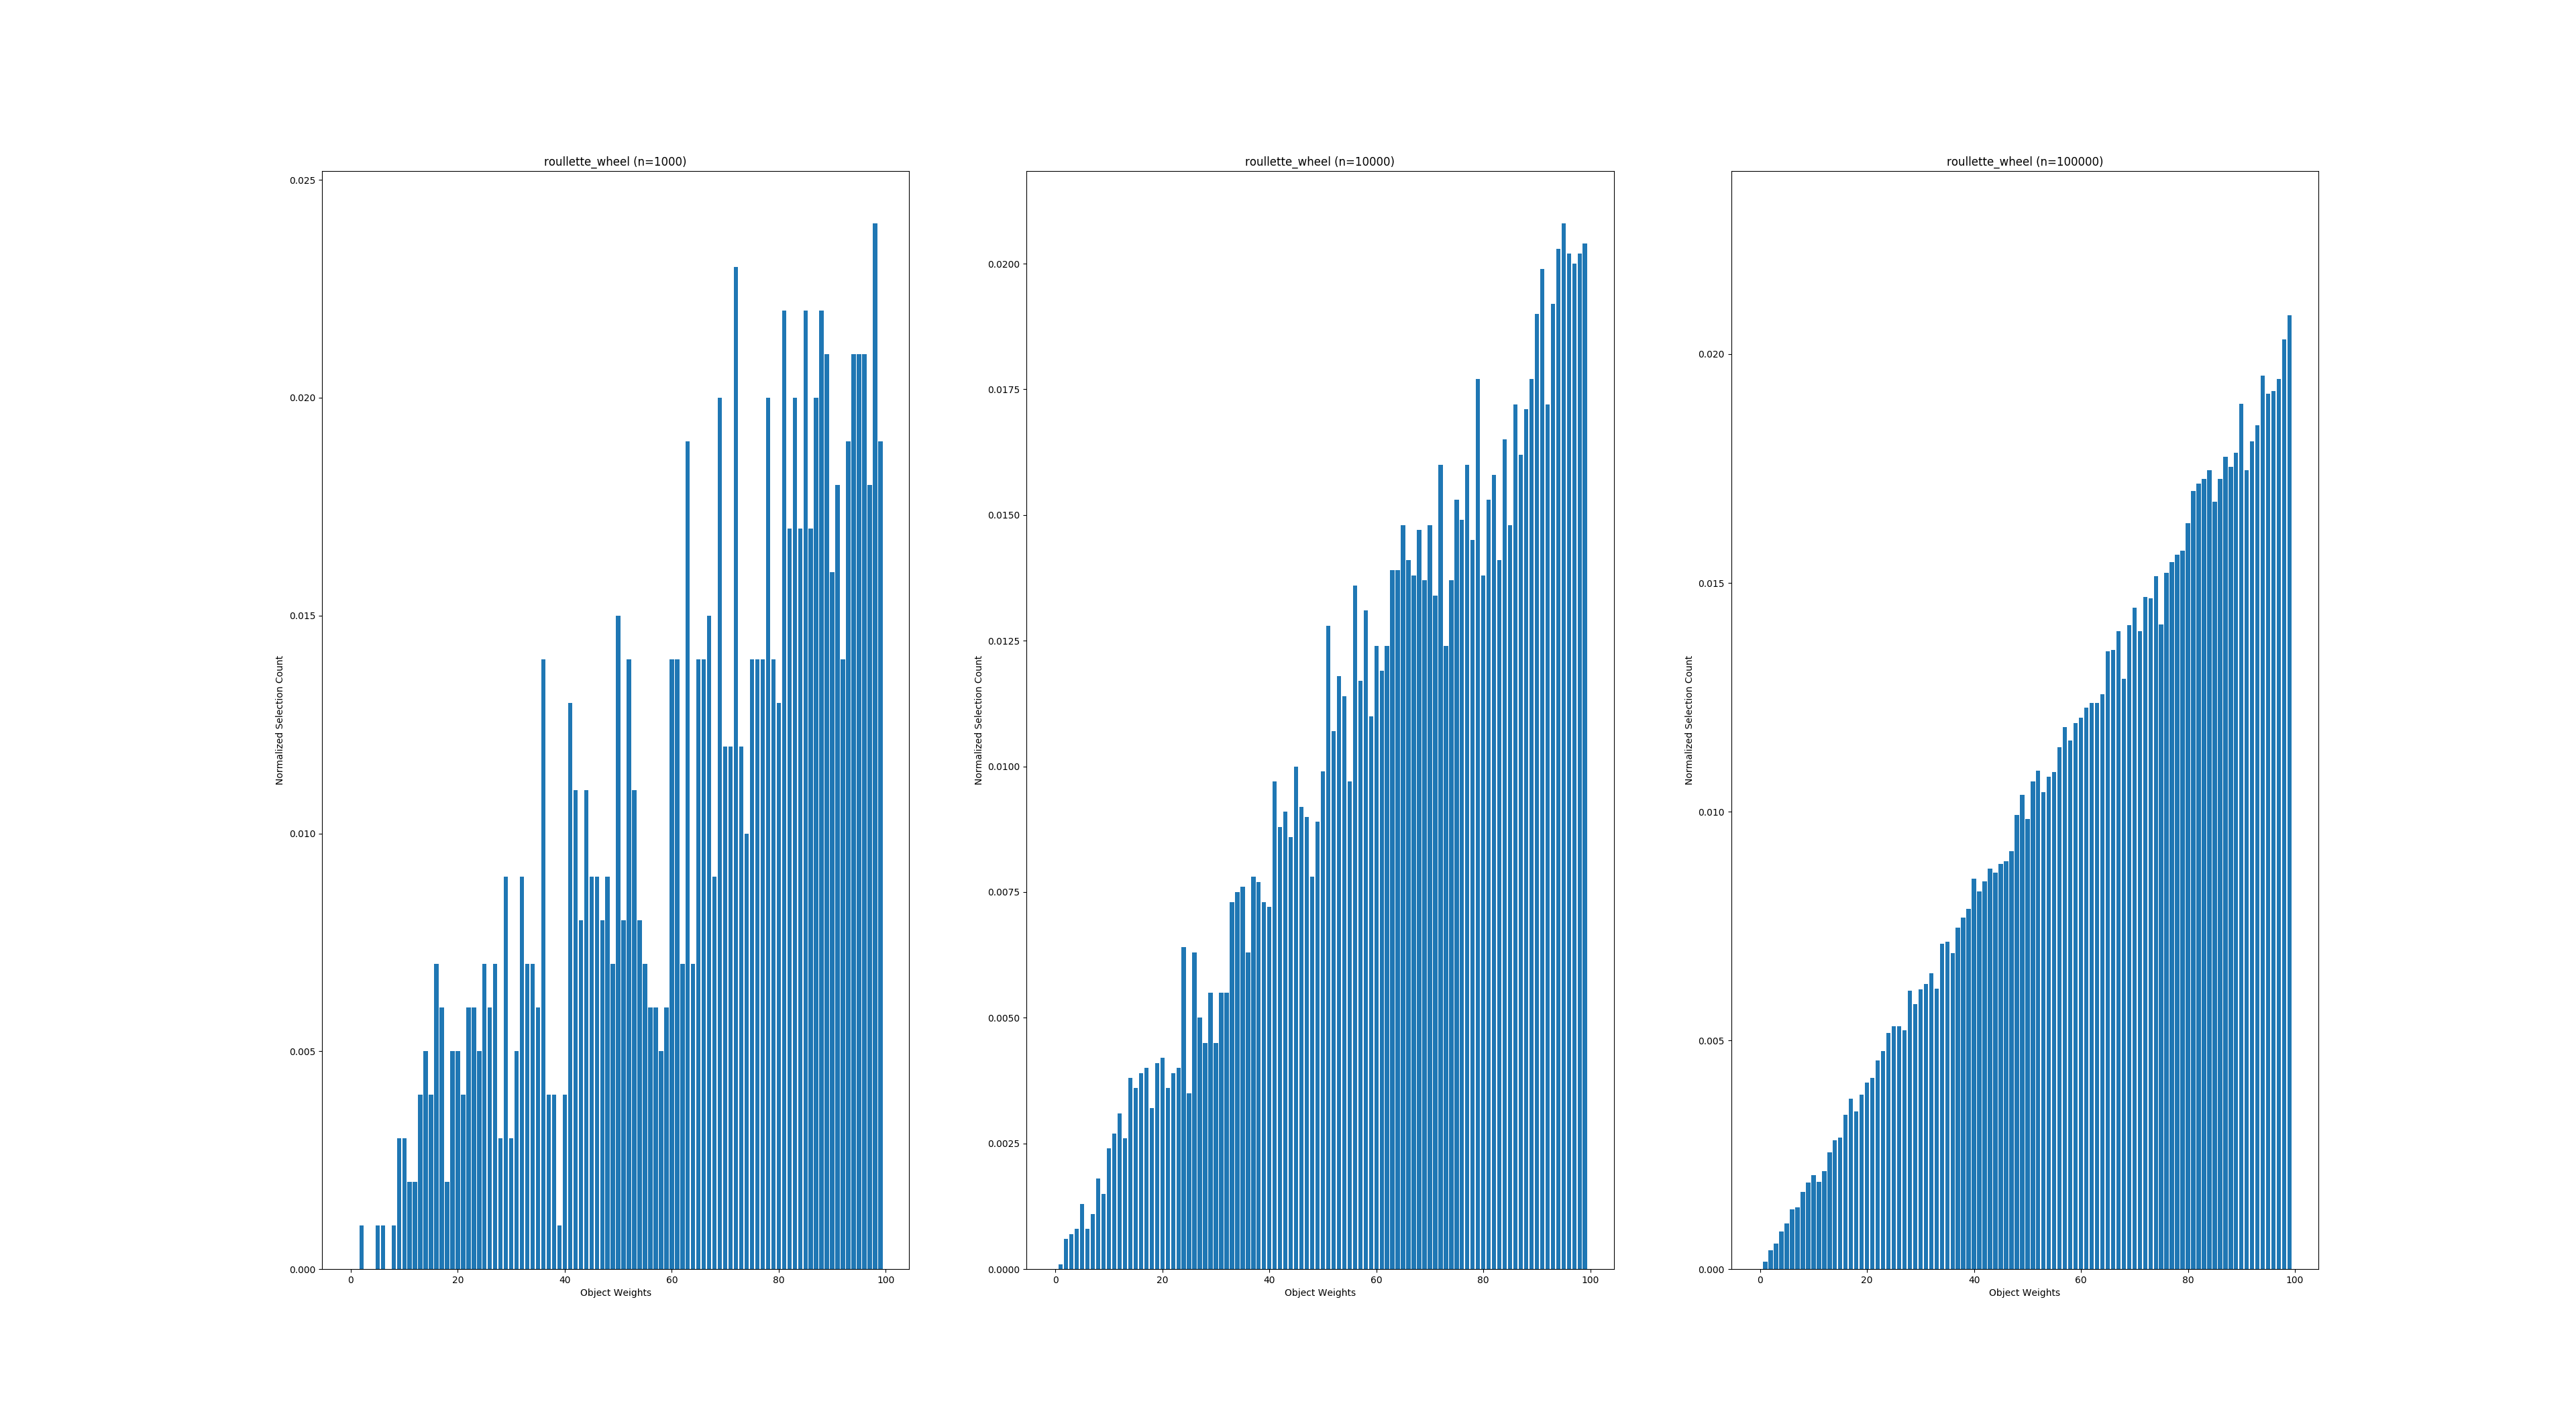
\includegraphics[scale=0.32]{images/herding_roullette.png} 
      \caption{Histograms generated by simulation of Stochastic Universal
               Sampling to illustrate selection distributions.}
      \label{fig:herding_roullette}
    \end{figure}

    \begin{figure}[htbp]
      \centering
      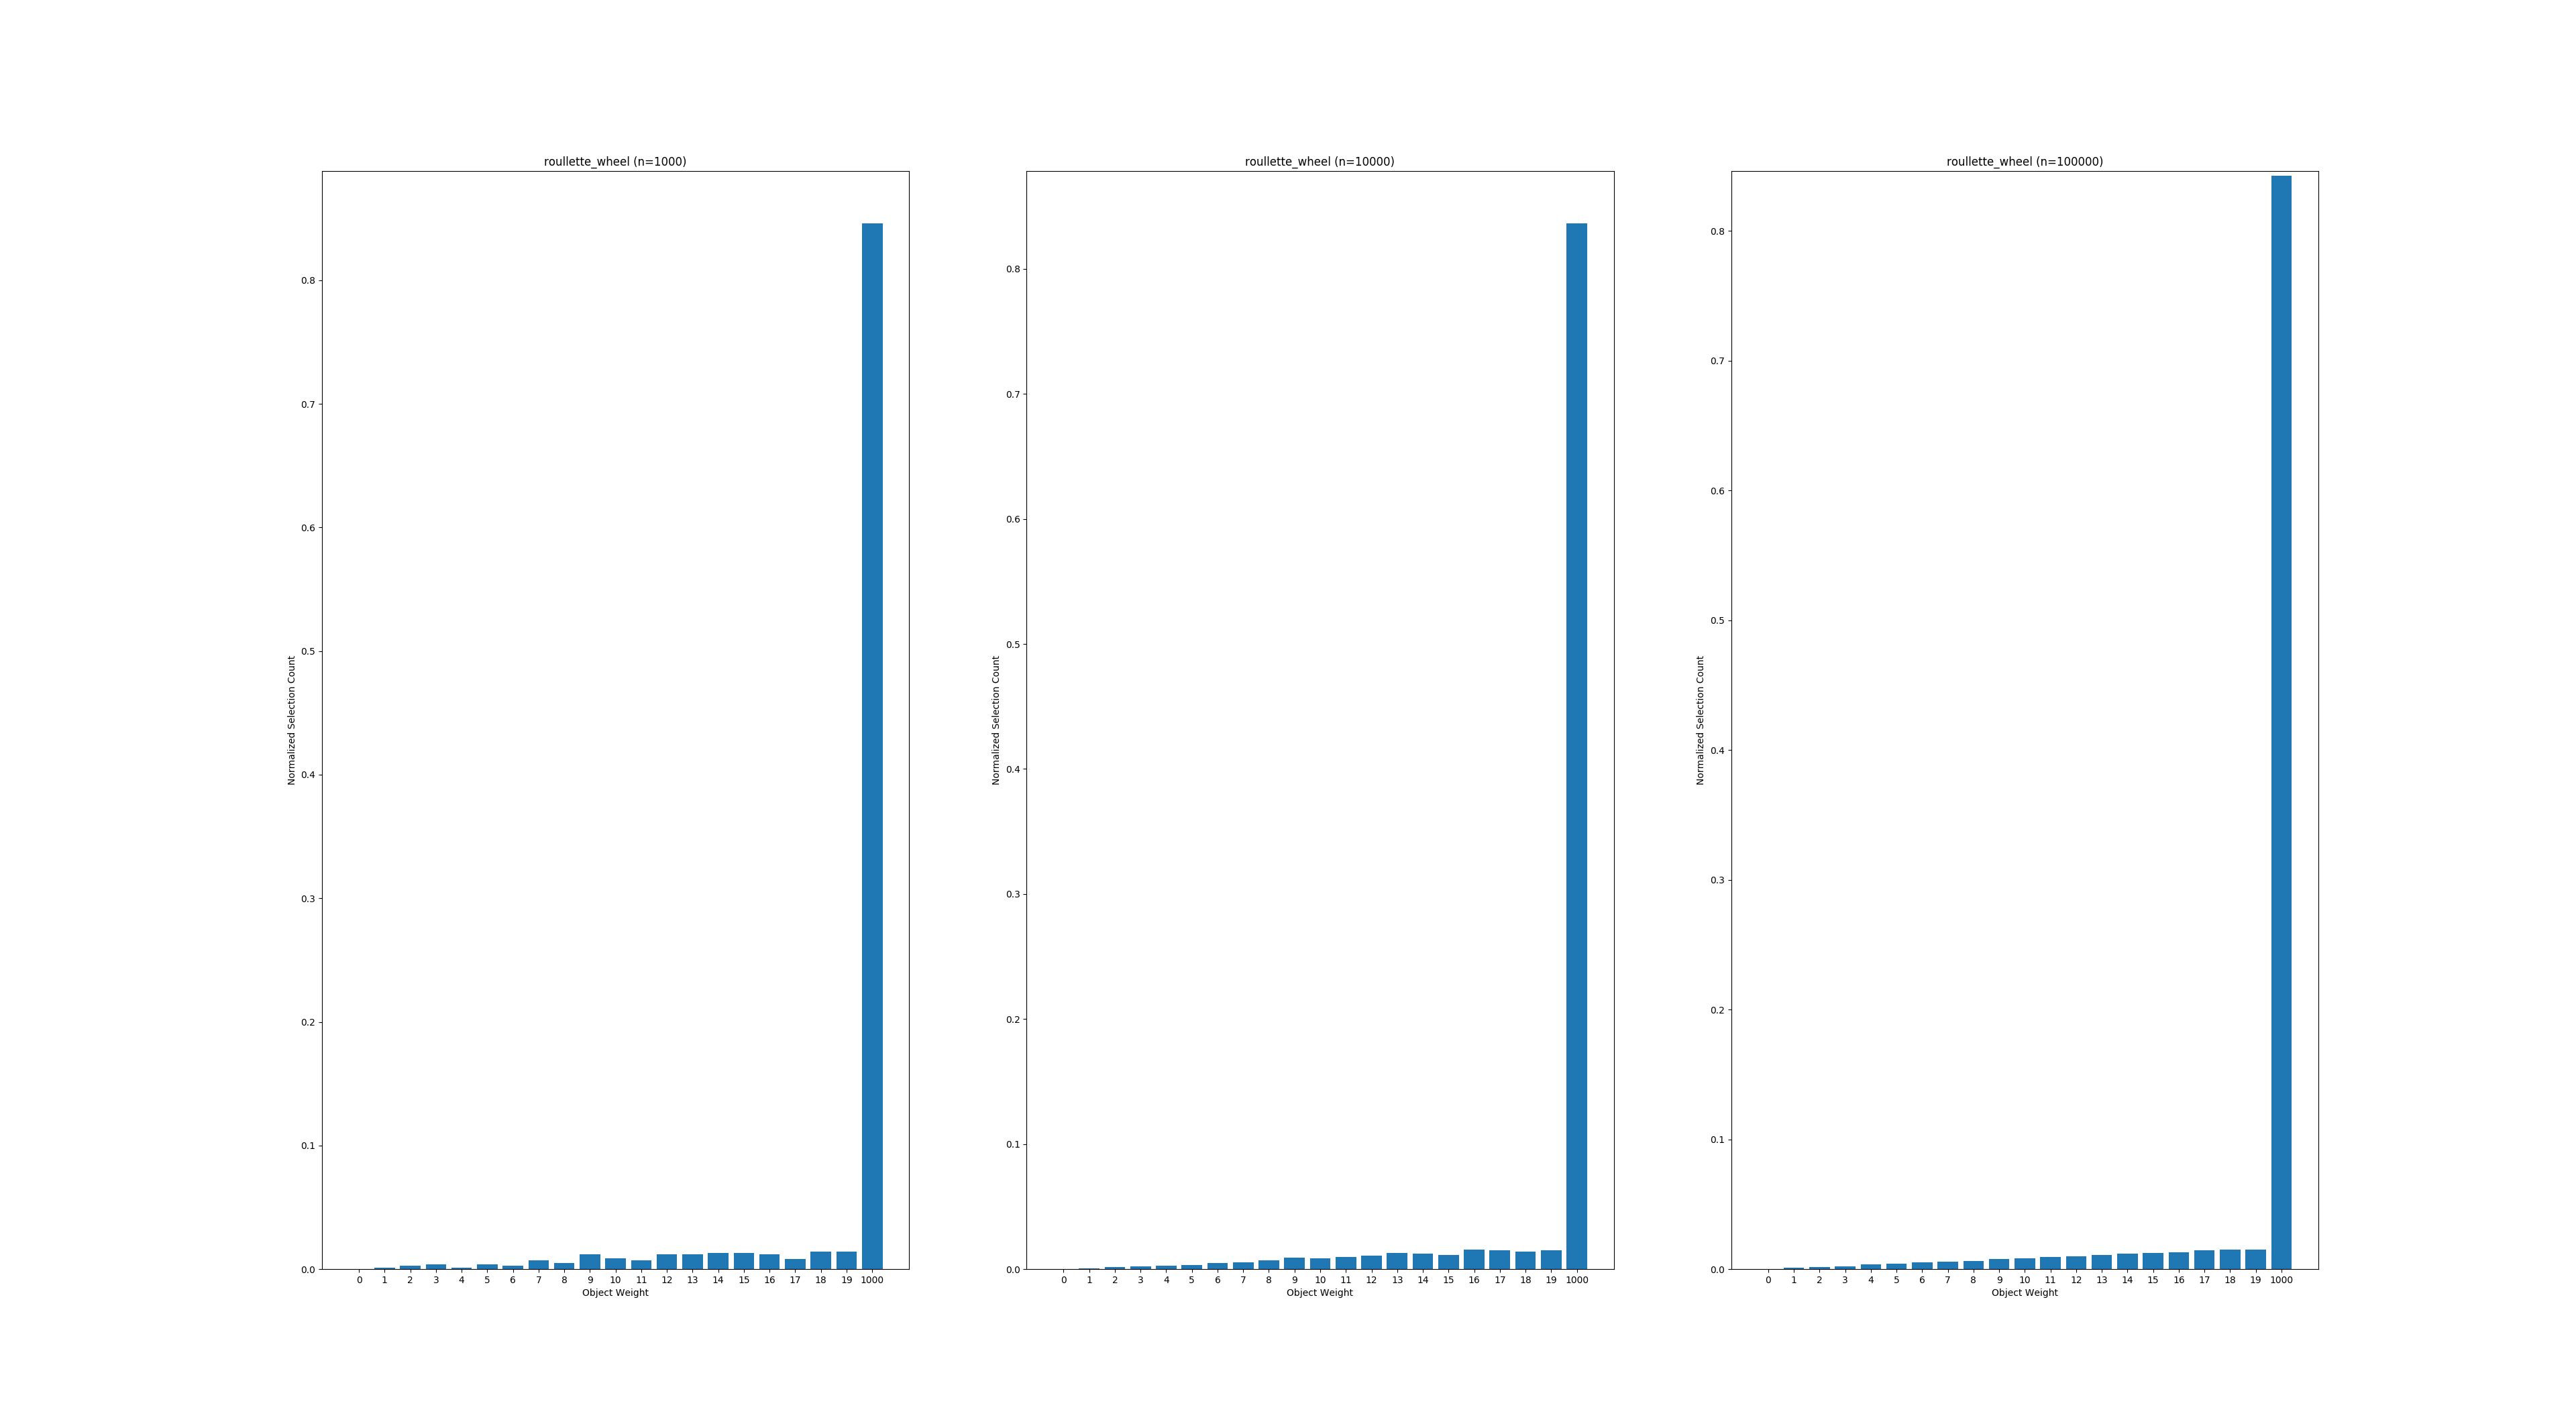
\includegraphics[scale=0.32]{images/pathological_roullette.png} 
      \caption{Histograms generated by simulation of Stochastic Universal
               Sampling to illustrate herding behavior.}
      \label{fig:pathological_roullette}
    \end{figure}

    Figure \ref{fig:herding_roullette} shows the evolution of the
    distribution of selection frequencies for SUS as the number of samples
    increases. It is evident that the selection frequency is proportional to the
    object weight. This can prove problematic for outlier objects with weights
    that are much larger than the other objects in the set as shown in Figure
    \ref{fig:pathological_roullette}. The high weight object's selection
    frequency eclipses all other objects in the selection pool which can lead
    to extreme herding behaviors.

    \subsubsection{Tructation Selection Simulations}
    Truncation selection \cite{truncation1973}, typically used in evolutionary
    computing algorithms, does not consider any objects for selection below
    some threshold, $T$. In Figure \ref{fig:herding_truncation}, only the top
    10\% of objects ranked by weight are considered for selection. Within this
    subset, weight has no meaning so there is a uniform distribution of
    selections. However, this may not be suitable for use cases where all
    objects must be candidates for selection.  Depending on the threshold
    chosen, this algorithm can be resistant to herding behavior as shown in
    Figure \ref{fig:pathological_truncation}. 

    \begin{figure}[htbp]
      \centering
      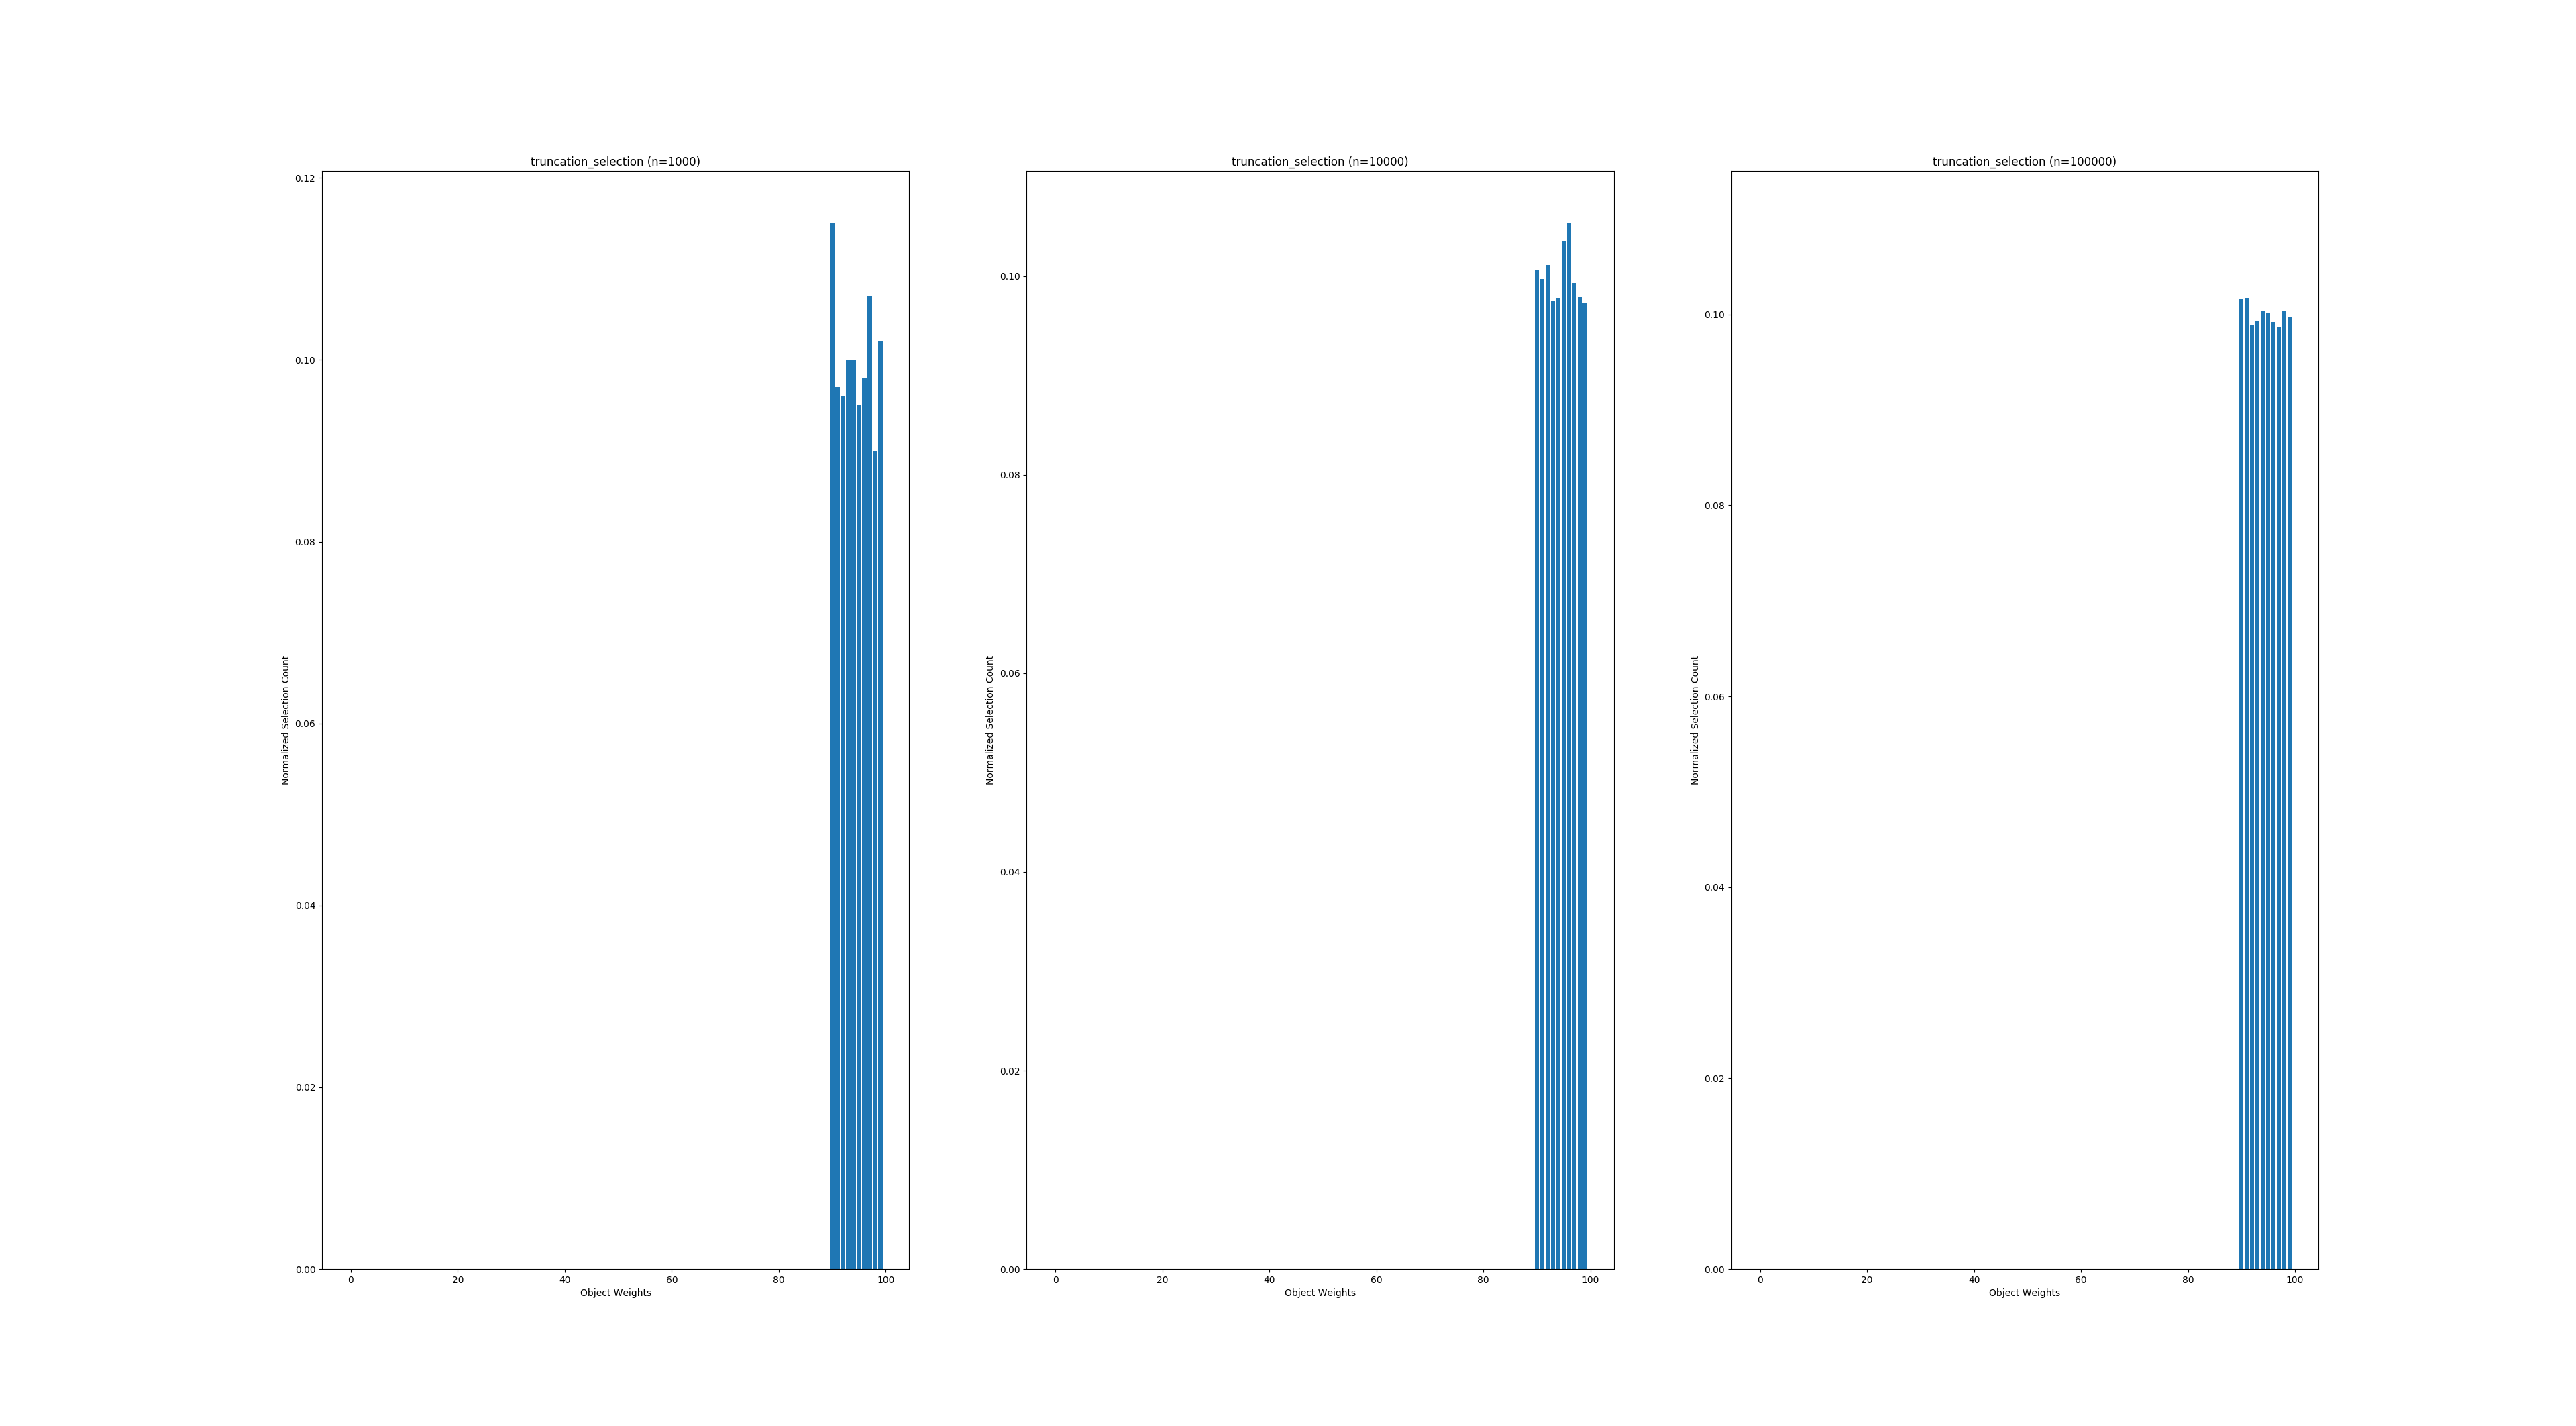
\includegraphics[scale=0.32]{images/herding_truncation.png} 
      \caption{Histograms generated by simulation of truncation selection
               to illustrate selection distributions.}
      \label{fig:herding_truncation}
    \end{figure}

    \begin{figure}[htbp]
      \centering
      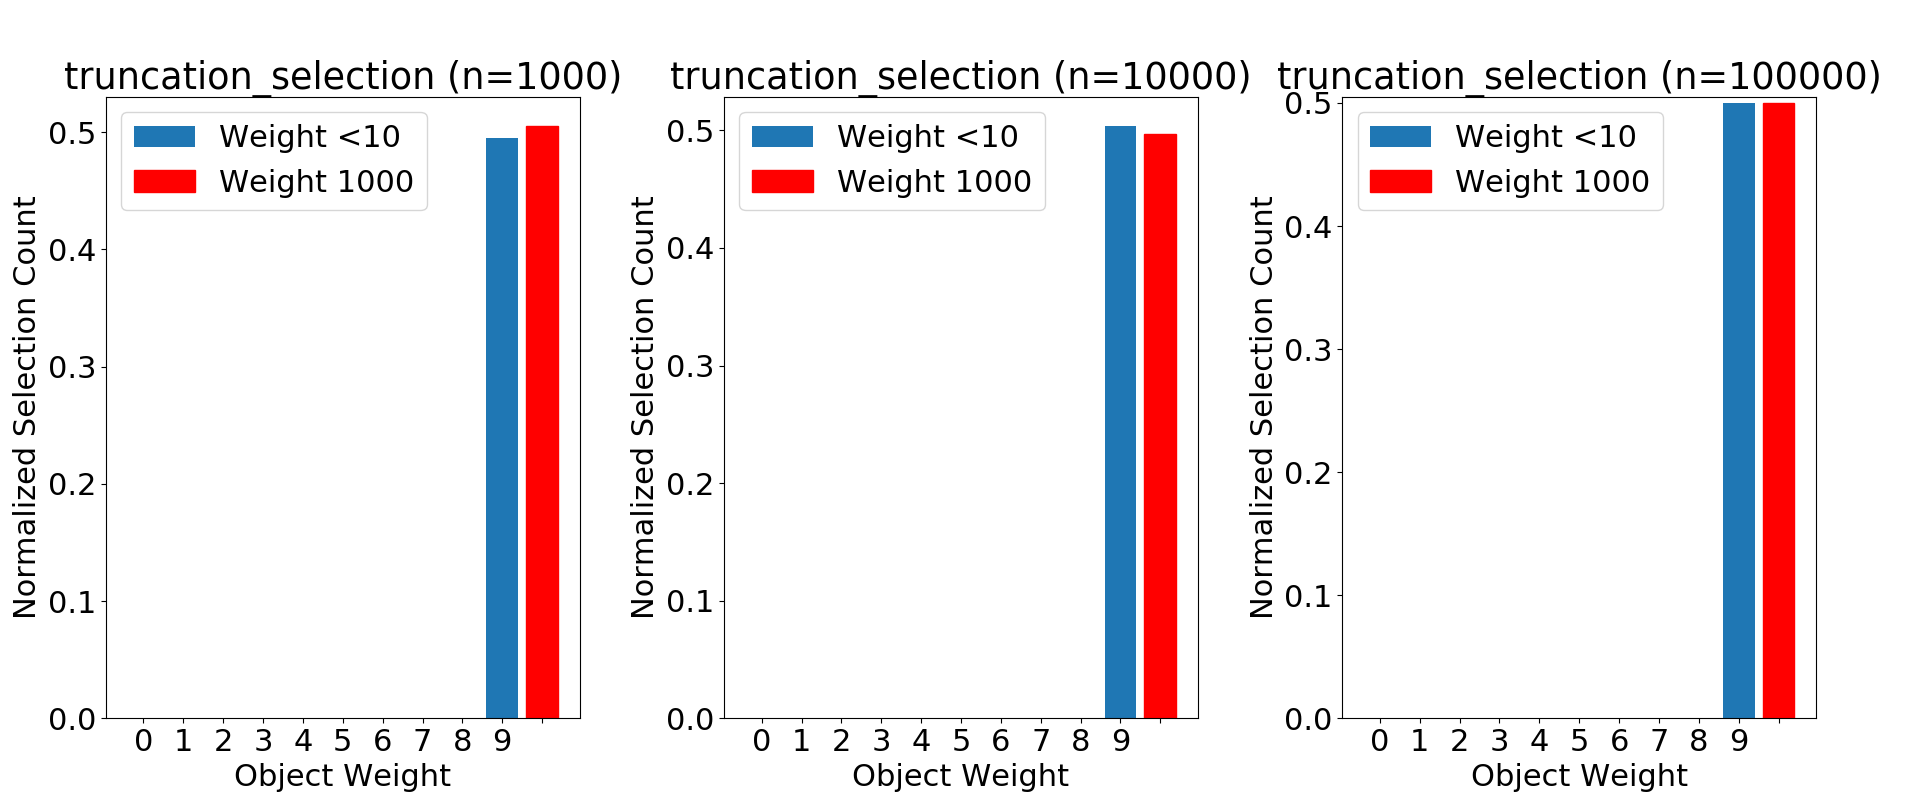
\includegraphics[scale=0.32]{images/pathological_truncation.png} 
      \caption{Histograms generated by simulation of truncation selection
               to illustrate herding behavior.}
      \label{fig:pathological_truncation}
    \end{figure}

    \subsubsection{Two-choice Sampling Simulations}
    Two-choice sampling \cite{2choice} performs a uniform random selection
    twice and returns the object with higher weight. This algorithm has shown
    to be extremely resilient to herding behavior as shown in Figure
    \ref{fig:pathological_two_choice} and selection frequencies for all objects
    are influenced by object weights in a way similar to SUS. While an object
    with a higher weight is more likely to be selected, it is not selected with
    a probability proportional to its fitness value. This makes the algorithm
    resistant to any herding behaviors, but will not be a good candidate if
    it's desired for the \texttt{WeightedVector} to select objects with
    probability proportional to its weight.

    \begin{figure}[htbp]
      \centering
      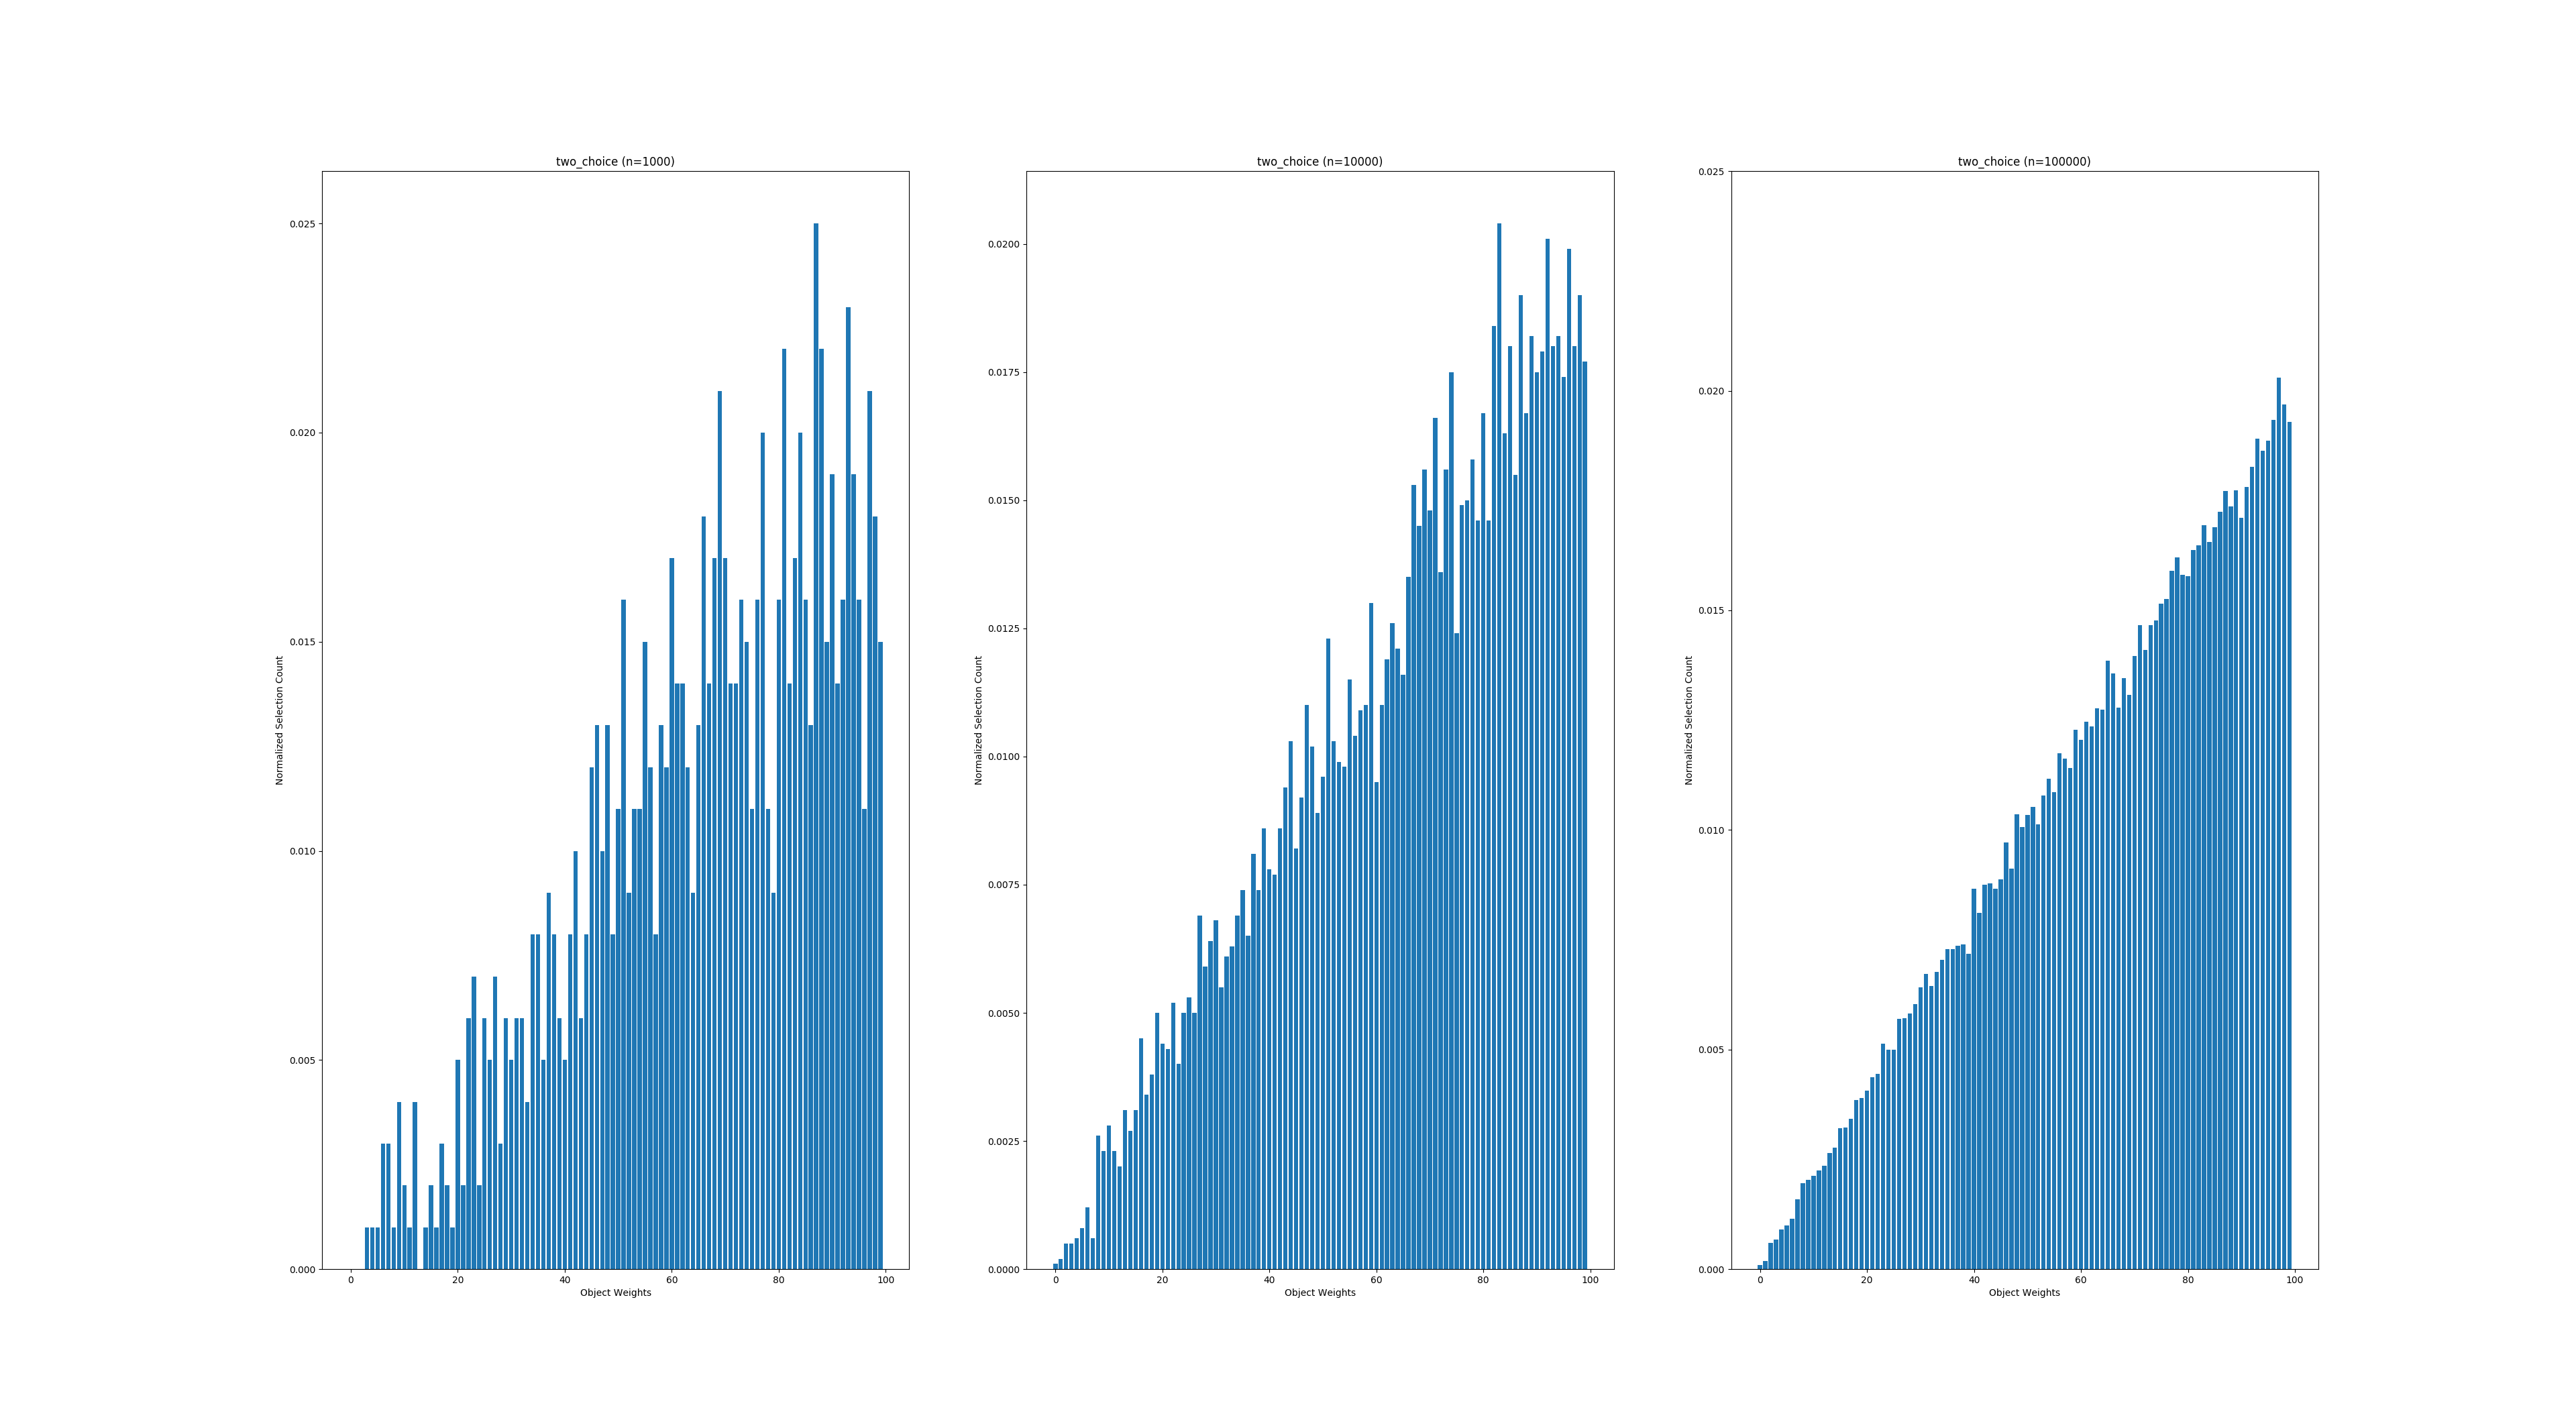
\includegraphics[scale=0.32]{images/herding_two_choice.png} 
      \caption{Histograms generated by simulation of two-choice selection
               to illustrate selection distributions.}
      \label{fig:herding_two_choice}
    \end{figure}

    \begin{figure}[htbp]
      \centering
      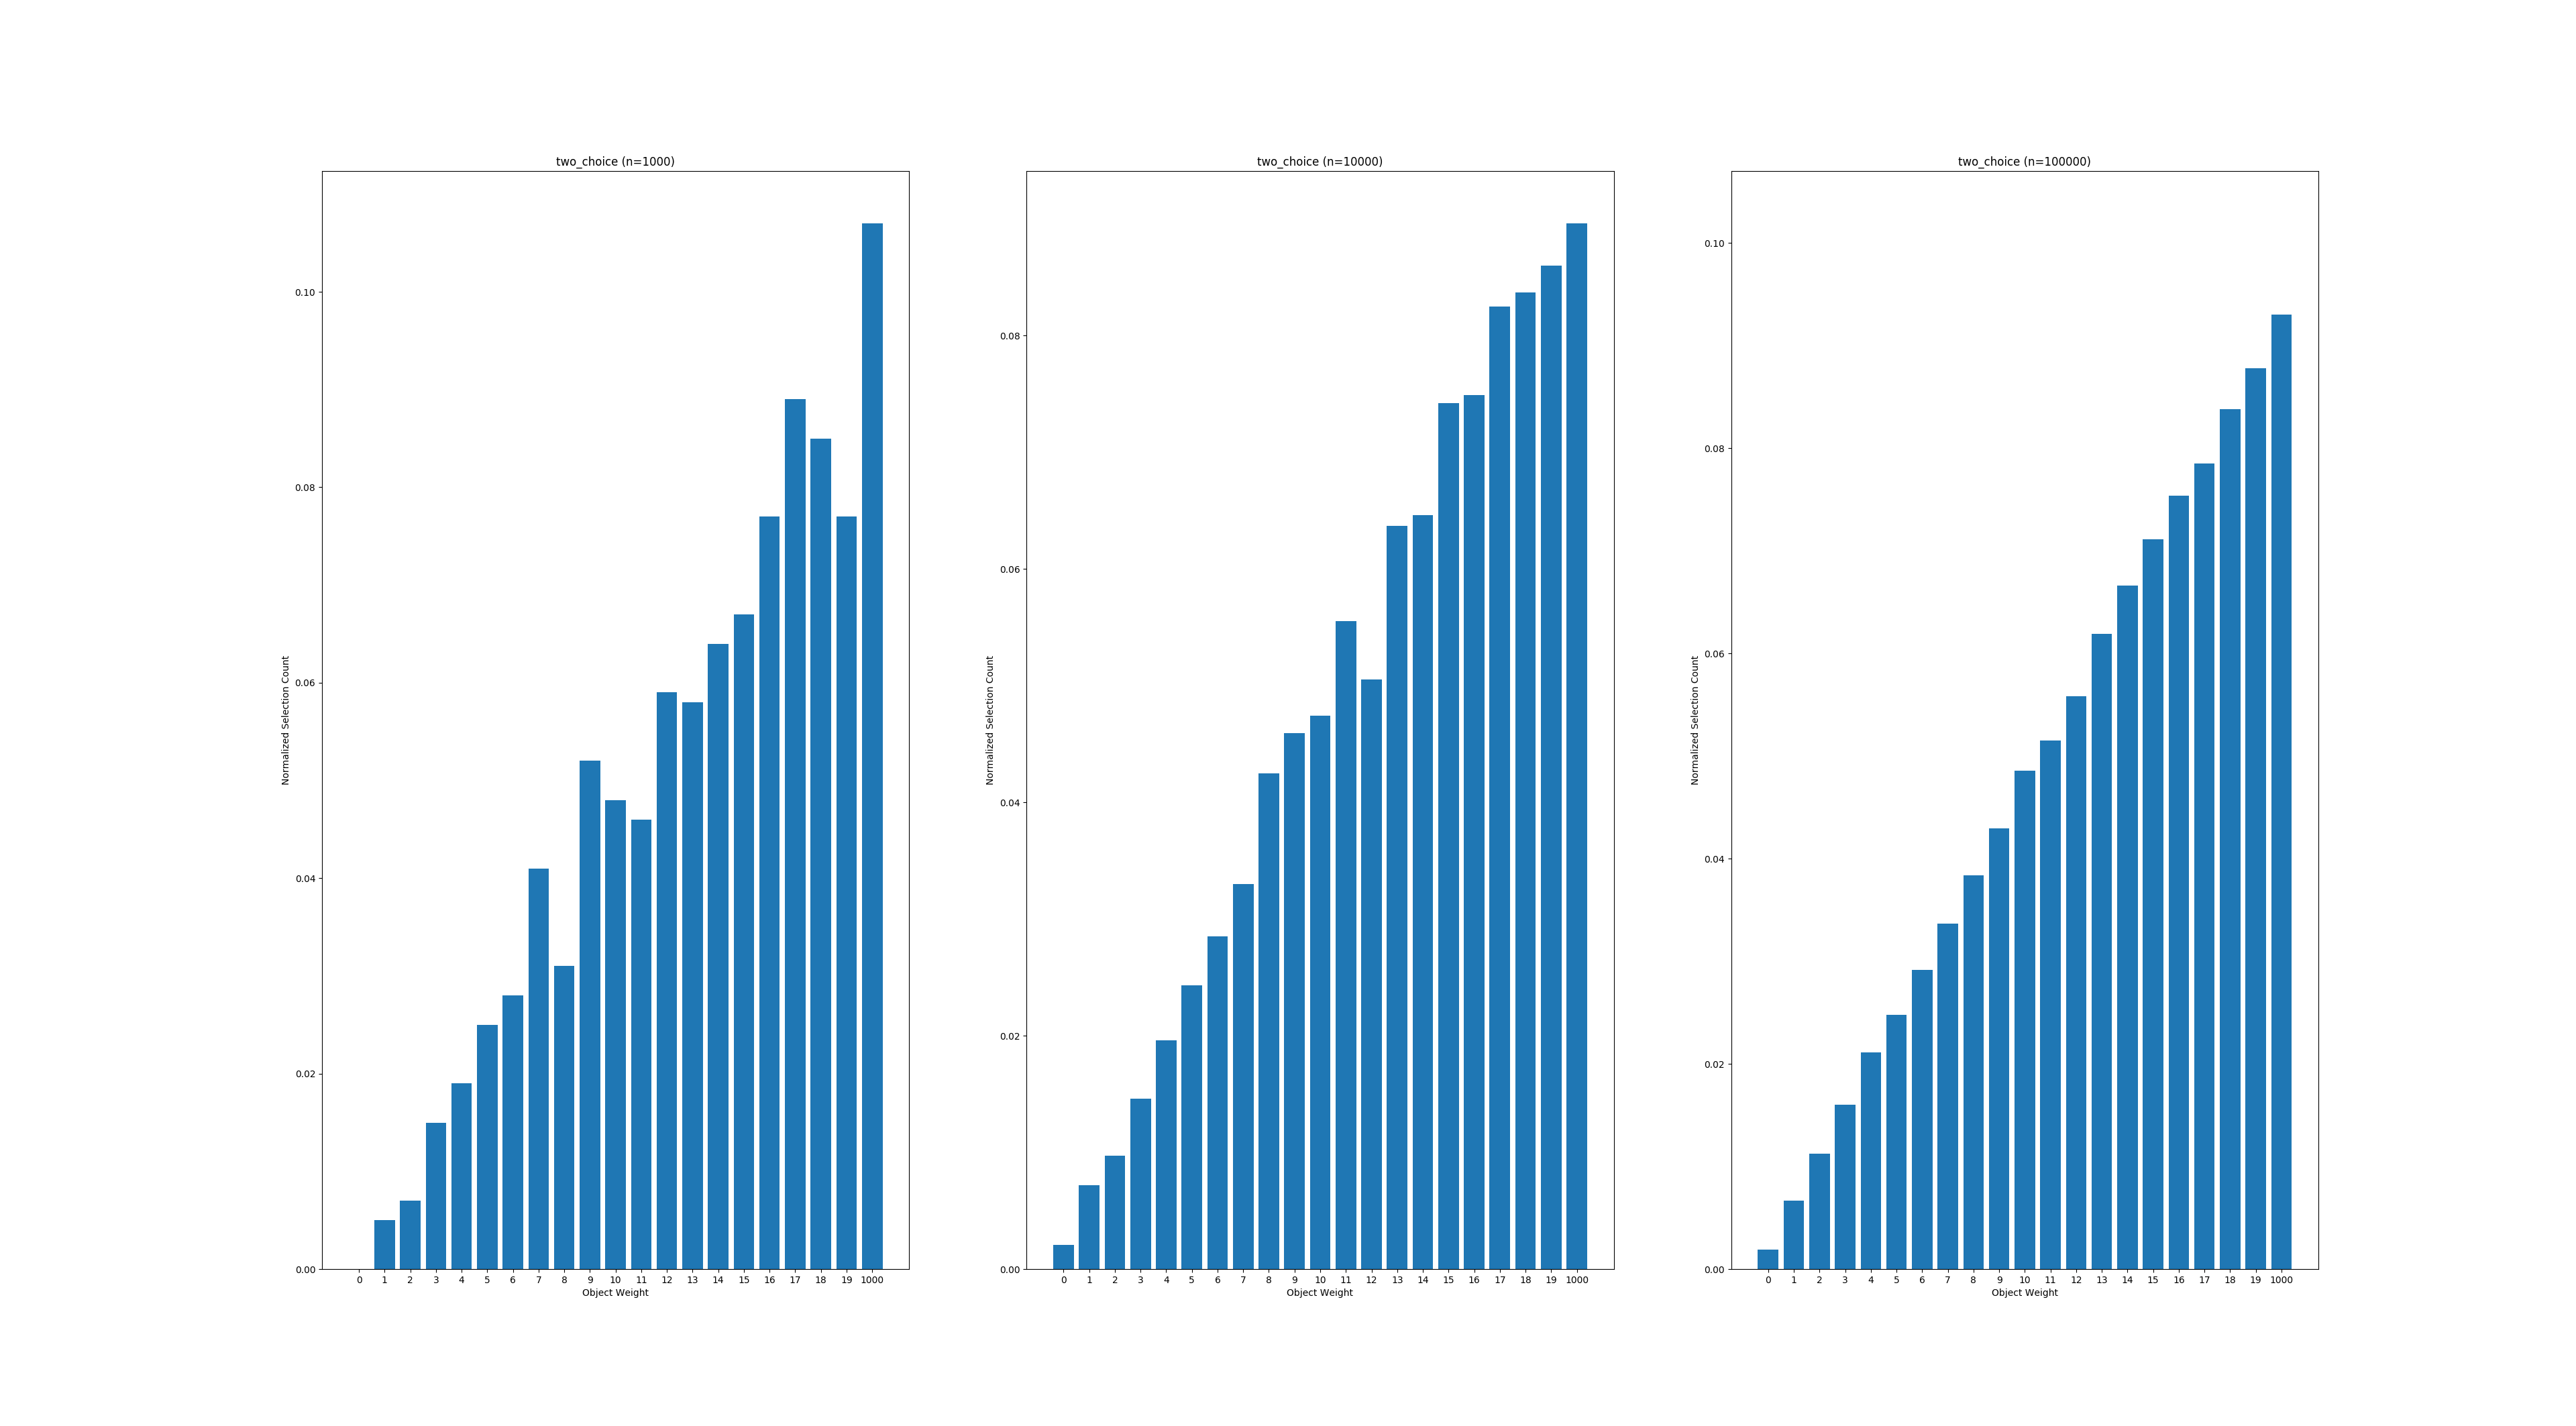
\includegraphics[scale=0.32]{images/pathological_two_choice.png} 
      \caption{Histograms generated by simulation of two-choice selection
               to illustrate herding behavior.}
      \label{fig:pathological_two_choice}
    \end{figure}

    \FloatBarrier

    \subsubsection{Uniform Random Selection Simulations}
    Uniform random selection is completely indifferent to object weights.
    Therefore, it exhibits no herding behavior and no usefulness for the
    \texttt{WeightedVector}'s sampling, but it is important to include its analysis for
    comparison with other selection algorithms.

    \begin{figure}[htbp]
      \centering
      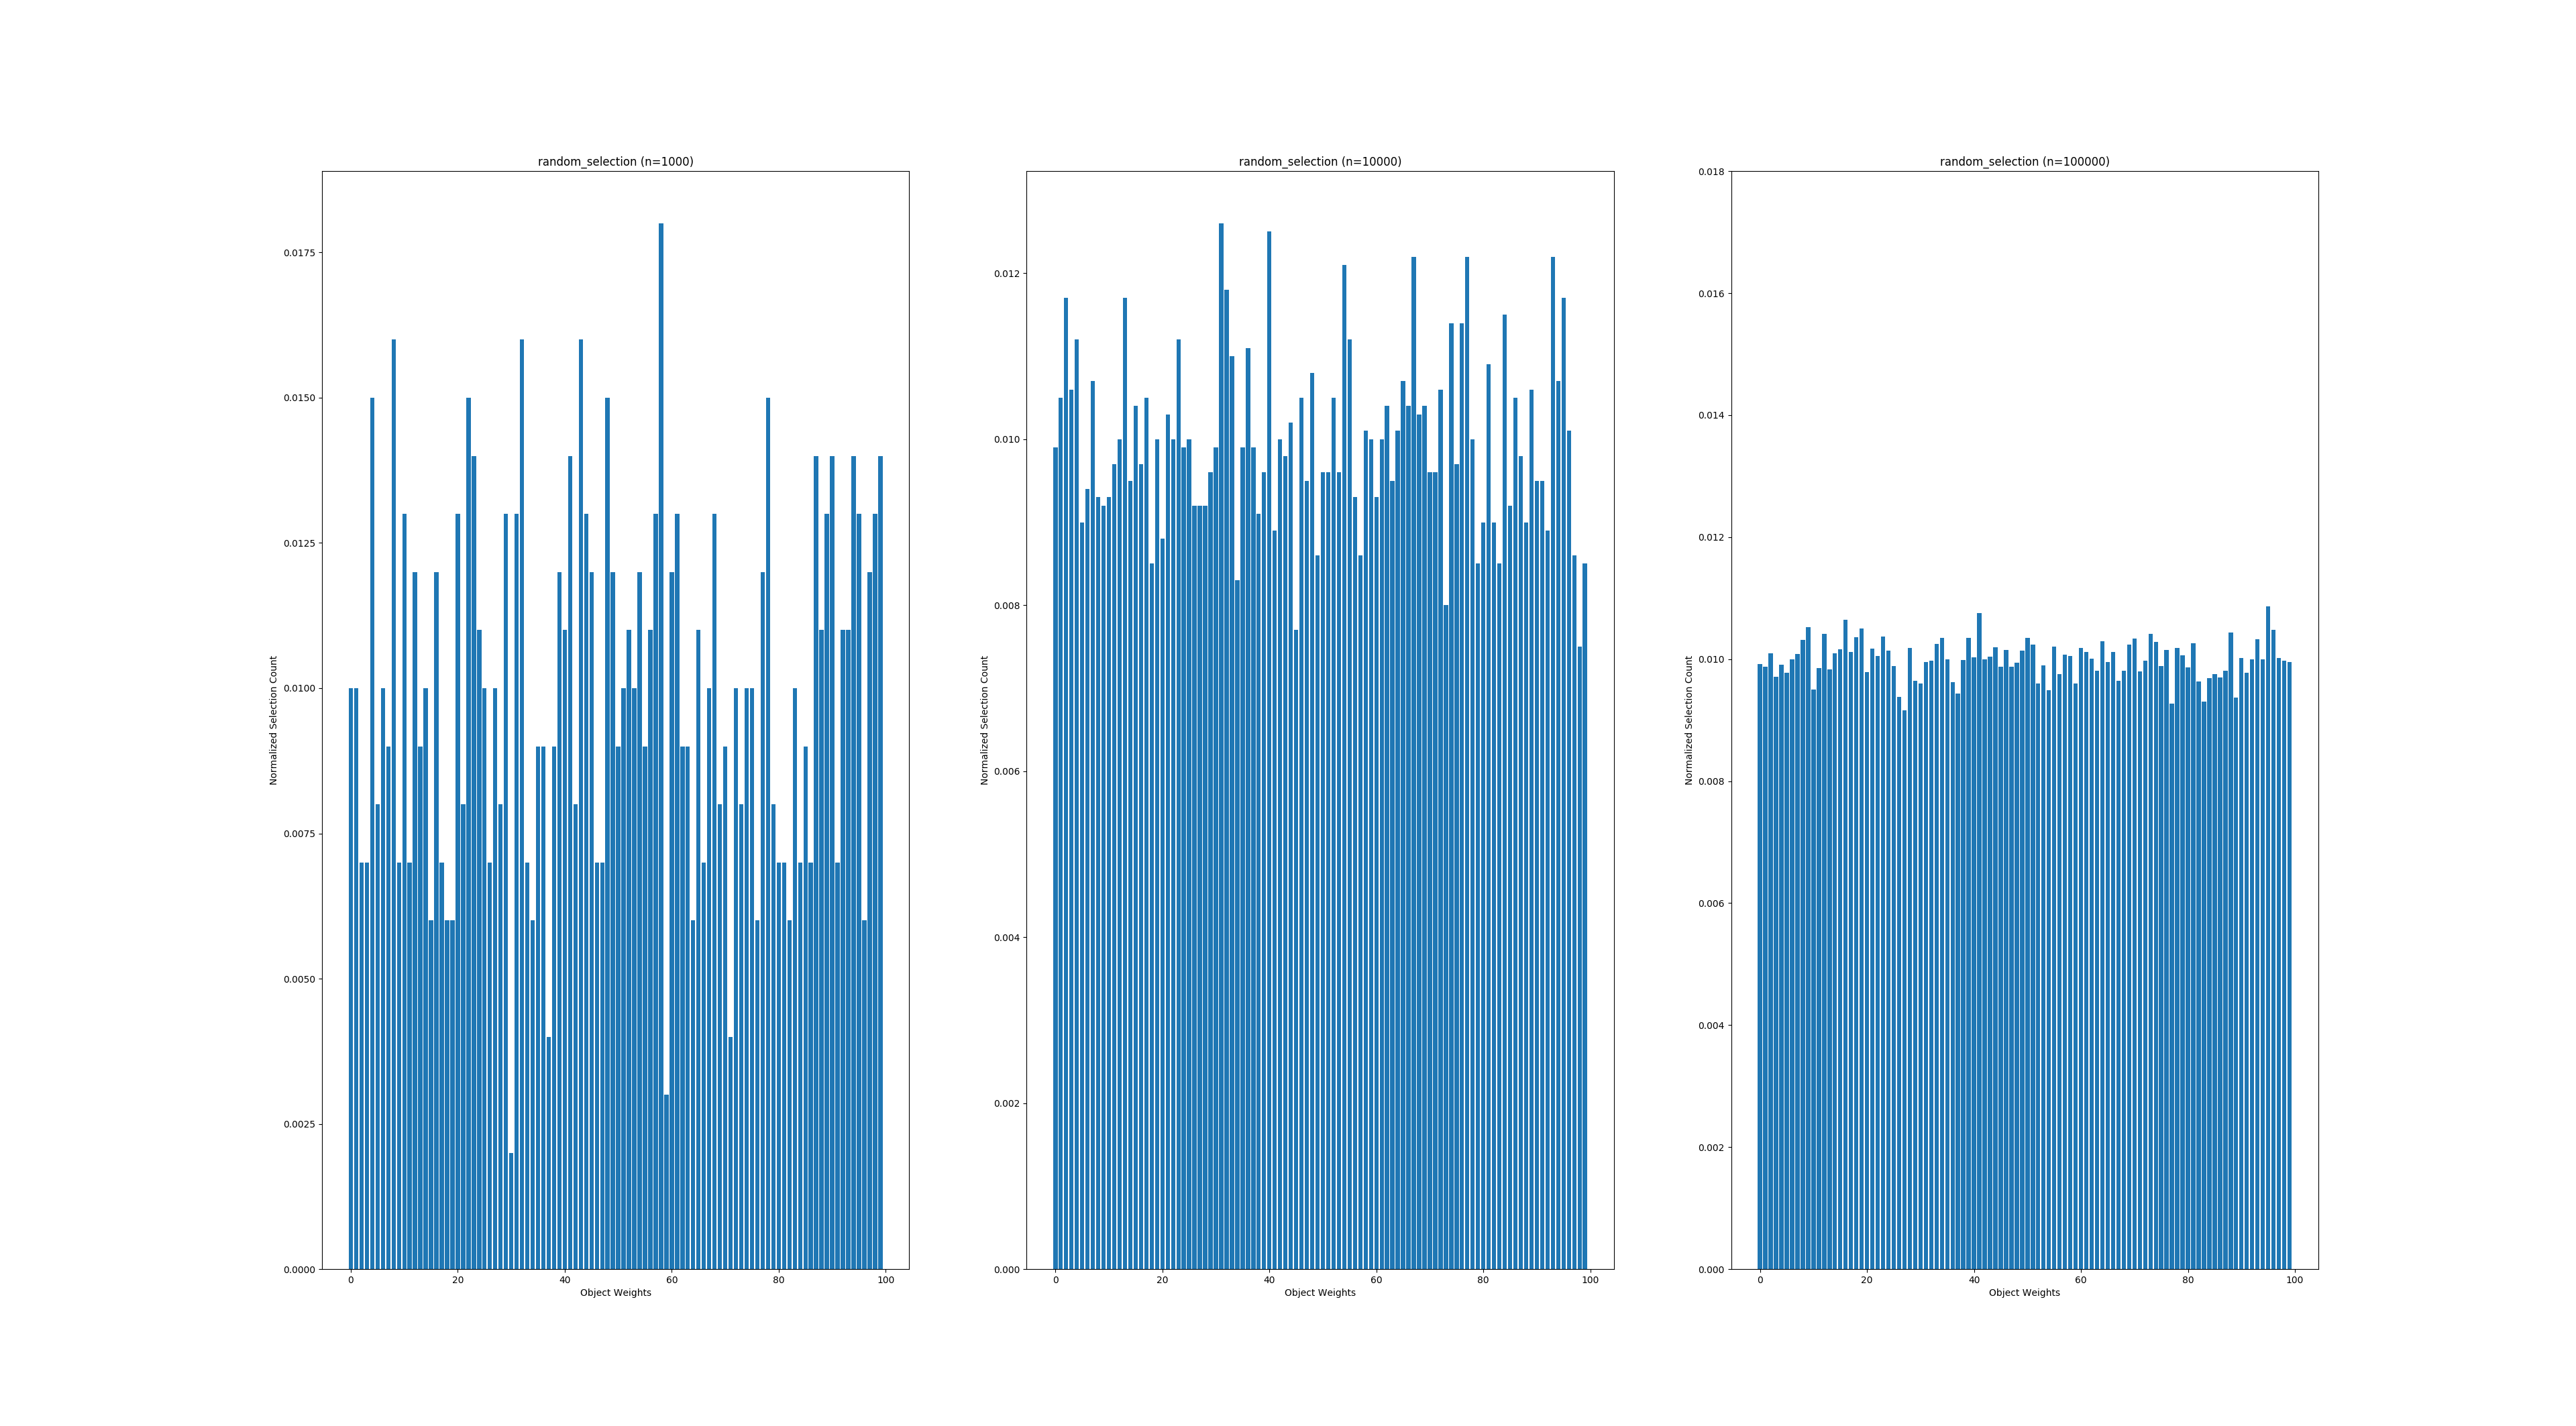
\includegraphics[scale=0.32]{images/herding_random.png} 
      \caption{Histograms generated by simulation of uniform random selection
               to illustrate selection distributions.}
      \label{fig:herding_random}
    \end{figure}

    \begin{figure}[htbp]
      \centering
      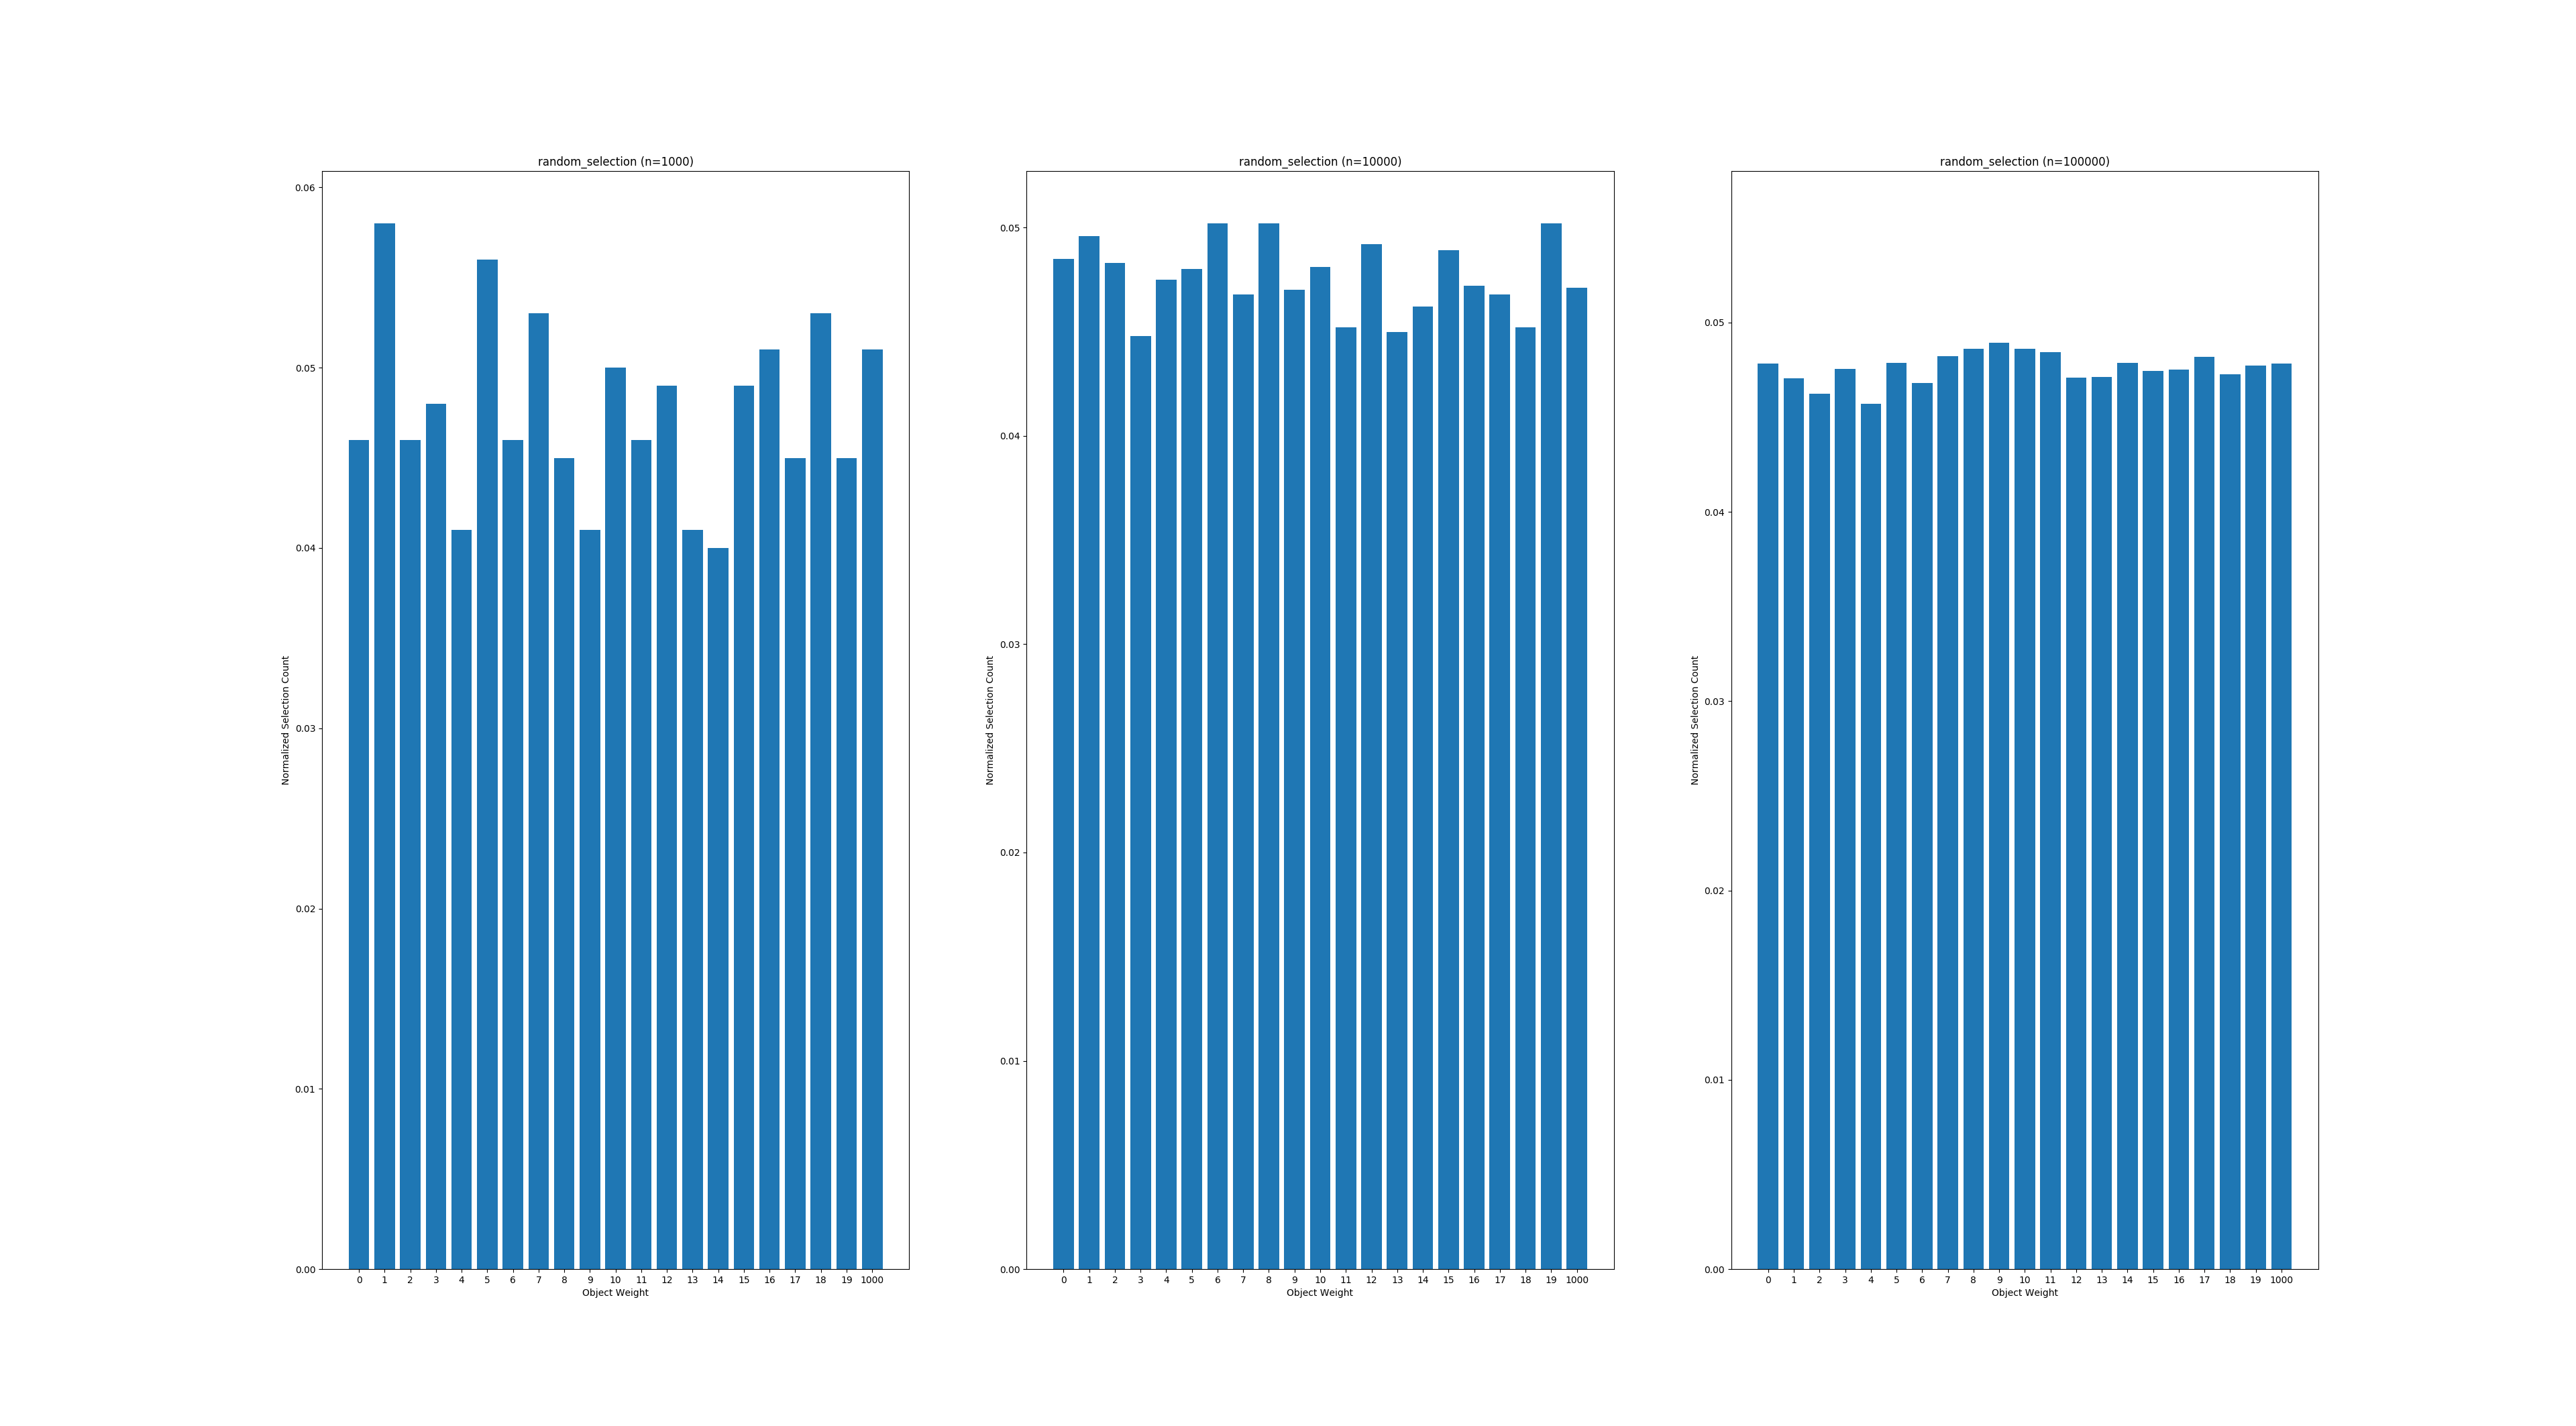
\includegraphics[scale=0.32]{images/pathological_random.png} 
      \caption{Histograms generated by simulation of uniform random selection
               to illustrate herding behavior.}
      \label{fig:pathological_random}
    \end{figure}

    Figure \ref{fig:pathological_truncation} shows that uniform selection
    probabilities can be expected and Figure \ref{fig:pathological_random}
    confirms there is no herding behavior with a uniform random selection
    scheme.

    \subsubsection{Weighted Random Algorithm Scalability Analysis}
    Even though both SUS and truncation selection have $O(N * D)$ time
    complexity, where $D$ is the number of objects in the set and $N$ is the number of
    selections required in one iteration, truncation selection is slower than
    SUS by an order of magnitude. This is mainly due to the need for the
    truncation selection algorithm to calculate the top T\% of the set for
    every selection performed in the simulations, an $O(Dlog(D))$ operation. As
    expected, two-choice and random selections are observed to be constant-time
    algorithms due to its simplicity of two uniform random selections.
    Two-choice is slightly slower than random selection due to the second
    uniform random selection and comparison operation that must occur before
    returning an object.

    \begin{figure}[htbp]
      \centering
      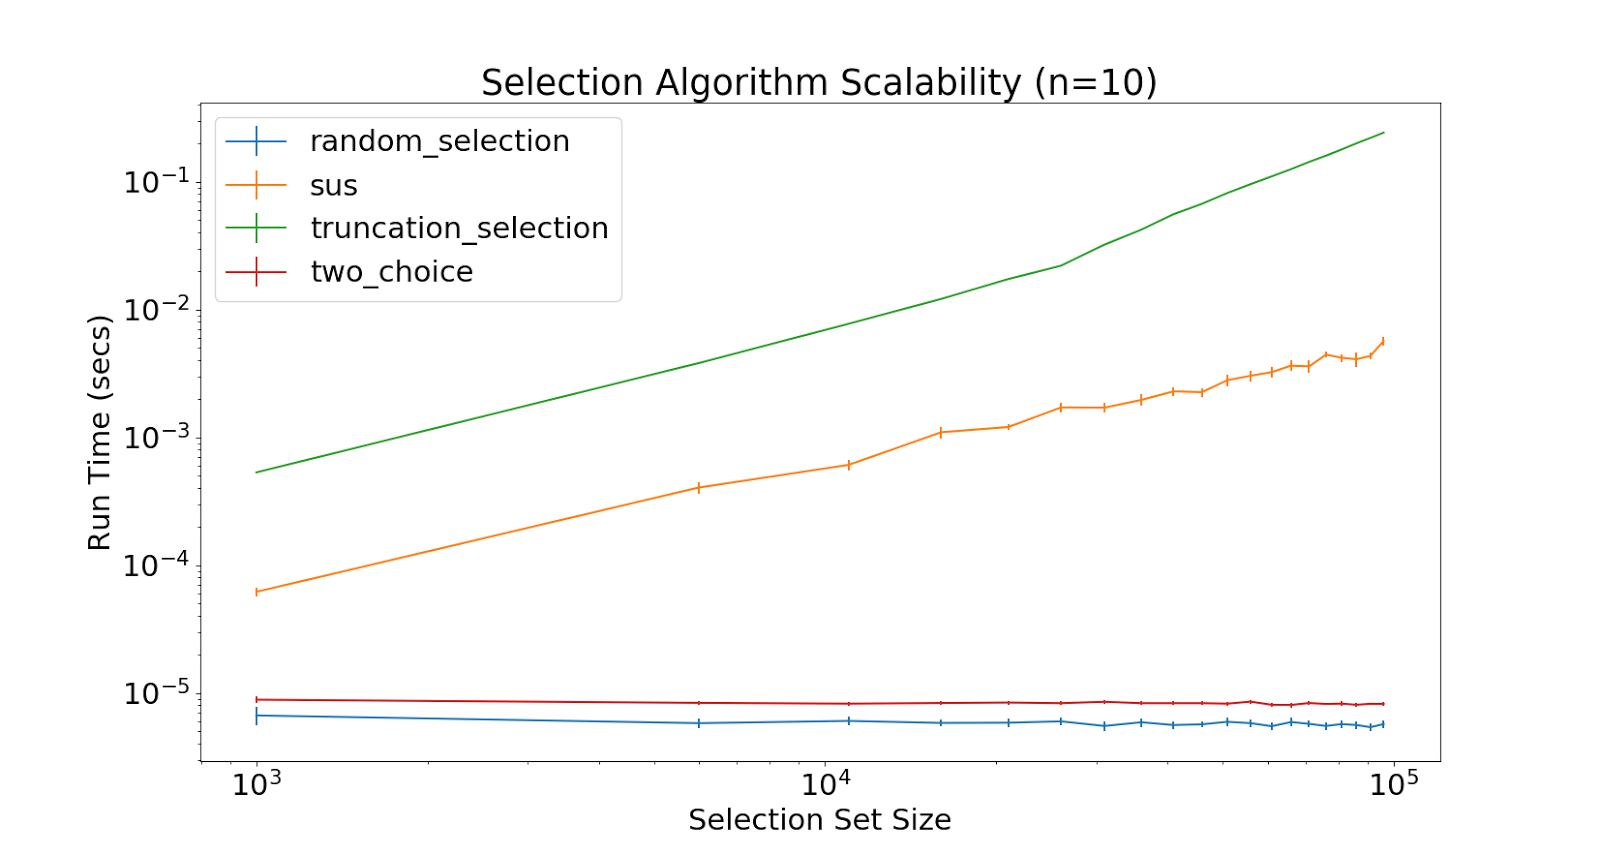
\includegraphics[scale=0.28]{images/random_scalability.png} 
      \caption{Running times of various weight random selection algorithms.}
      \label{fig:random_scalability}
    \end{figure}

    Figure \ref{fig:random_scalability} shows the running times for each of
    the weighted random selection algorithms discussed. It becomes clear that
    weighted random selections for large sets of objects is most efficient
    using a two-choice sampling technique.

  \subsection{WeightedVector Class}

  It is cleaner to implement repeated weighted sampling of disk IDs in such a
  way that we call a single function to return a set of unique disk IDs from a
  sampling set using a weighted random sampling algorithm that uses the disks'
  fitness values. An object container class is needed similar to the data
  structures in the C++ Standard Template Library \cite{stl}. A requirement for
  this object is that must be able to access elements of arbitrary types via
  arbitrary weighted random sampling methods. The \texttt{WeightedVector} class
  was implemented to fulfill this requirement. 

  Upon instantiation of the \texttt{WeightedVector} class, a fitness function
  is provided to store the fitness values of all objects internally. The
  \texttt{WeightedVector} class has implemented insertion, removal, and
  weighted random sampling of objects of some arbitrary type, $T$, based on the
  object's fitness value as a weight.

  The set of objects and their fitness values are stored in
  \texttt{std::vector} objects, one for the object references stored in the
  \texttt{WeightedVector} and one for their corresponding fitness values. The
  objects and their corresponding fitness values share an index into their
  respective internal vectors.

  \begin{table}[htbp]
    \caption{WeightedVector public interface.}
    \label{tab:wvpub}
    \begin{tabular}{ | p{1.0\linewidth} | }
      \hline
      \verb|WeightedVector(const std::function<double(const T)>)| \\ \hline
      The \texttt{WeightedVector} class is instantiated by providing a fitness function
      that accepts a reference to an object of type \emph{T} and returns a
      fitness value that is of type \emph{double}. The provided fitness function
      is used to create a mapping between inserted objects and their
      corresponding fitness values for sampling.

      The \texttt{WeightedVector} class asserts that the fitness function returns positive
      values. \\ \hline

      \\ \hline

      \verb|void EmplaceBack(const T& element)| \\ \hline
      The EmplaceBack function constructs and inserts an object of type
      \emph{T} at the end of the vector. This increases the WeightedVector's
      size by 1. \\ \hline

      \\ \hline

      \verb|bool Empty()| \\ \hline
      Returns true if the \texttt{WeightedVector} is of size 0. \\  \hline

      \\ \hline

      \verb|void Clear()| \\ \hline
      Resets all state in the \texttt{WeightedVector} object, sets the size to 0, and
      clears all internal vectors. \\ \hline

      \\ \hline

      \verb|T& Sample()|\\ \hline

      Returns a reference to an object stored inside of the WeightedVector.
      Objects are sampled via weighted random selection and subsequent calls to
      Sample are guaranteed not to return the same object unless Reset is called
      before sampling again. The \texttt{WeightedVector} class asserts that Sample is not
      called more times than the size of the WeightedVector.\\ \hline

      \\ \hline

      \verb|void Reset()|\\ \hline

      Resets the sampling state of the WeightedVector, allowing sampled objects
      to be eligible for selection in subsequent Sample calls.\\ \hline

      \\ \hline

      \verb|size_t size()|\\ \hline

      Returns the size of the WeightedVector.\\ \hline
    \end{tabular}
  \end{table}

  Table \ref{tab:wvpub} shows the \texttt{WeightedVector} public interface.

  \FloatBarrier

    \subsubsection{Weighted Vector Internals}

    Internally, the \texttt{WeightedVector} class keeps 3 different std:vector
    objects to keep track of sampling state and the object-to-fitness value
    mapping.  There is the \texttt{inner\_vector\_} variable which stores the
    objects inserted via \texttt{EmplaceBack()}, the \texttt{weights\_}
    variable which stores the fitness values of all objects in the
    \texttt{inner\_vector\_}, and the \texttt{sampling\_weights\_} variable
    which is identical to \texttt{weights\_} except that objects weights are
    set to 0 when sampled. This allows us to exclude objects from being sampled
    multiple times between calls to \texttt{Reset()} with time complexity
    $O(1)$, since a weight of 0 gives a probability of 0 for sampling using
    Stochastic Universal Sampling as shown in the example below.

    Before sampling, there are identical \texttt{weights\_} and
    \texttt{sampling\_weights\_} vectors accompanying an
    \texttt{inner\_vector\_} of objects as shown in Table
    \ref{tbl:inner-vec-1}.

    \begin{table}[htbp]
      \caption{Inner vector example part 1.}
      \label{tbl:inner-vec-1}
      \begin{center}
      \begin{tabular}{ | l | c | c | c | r | }
        \hline
        \verb|inner_vector_| & $A$ & $B$ & $C$ & $D$ \\ \hline
        \verb|weights_| & 1 & 3 & 3 & 7 \\ \hline
        \verb|sampling_weights_| & 1 & 3 & 3 & 7 \\ \hline
        \hline
      \end{tabular}
      \end{center}
    \end{table}

    \FloatBarrier

    Suppose that a call to Sample() on the \texttt{WeightedVector} returns $D$. The
    probability of this event is 0.5, so to maintain sampling state within the
    WeightedVector, the weight associated with object $D$ is set to zero in
    Table \ref{tbl:inner-vec-2}.

    \begin{table}[htbp]
      \caption{Inner vector example part 2.}
      \label{tbl:inner-vec-2}
      \begin{center}
      \begin{tabular}{ | l | c | c | c | r | }
        \hline
        \verb|inner_vector_| & $A$ & $B$ & $C$ & $D$ \\ \hline
        \verb|weights_| & 1 & 3 & 3 & 7 \\ \hline
        \verb|sampling_weights_| & 1 & 3 & 3 & 0 \\ \hline
        \hline
      \end{tabular}
      \end{center}
    \end{table}

    \FloatBarrier

    If \texttt{Sample()} is called again, it is not possible to return $D$ since its
    sampling weight is now zero. The probabilities of returning $A$, $B$, or
    $C$ in subsequent calls to \texttt{Sample()} are $\frac{1}{7}$, $\frac{3}{7}$, and
    $\frac{3}{7}$ respectively. Suppose two more calls to \texttt{Sample()} lead to the
    state in Table \ref{tbl:inner-vec-3}.

    \begin{table}[htbp]
      \caption{Inner vector example part 3.}
      \label{tbl:inner-vec-3}
      \begin{center}
      \begin{tabular}{ | l | c | c | c | r | }
        \hline
        \verb|inner_vector_| & $A$ & $B$ & $C$ & $D$ \\ \hline
        \verb|weights_| & 1 & 3 & 3 & 7 \\ \hline
        \verb|sampling_weights_| & 0 & 3 & 0 & 0 \\ \hline
        \hline
      \end{tabular}
      \end{center}
    \end{table}

    \FloatBarrier

    There can only be one more call to \texttt{Sample()} without triggering an
    assertion failure and the \texttt{WeightedVector} is obligated to return
    $B$. The only way to restore sampling state is to call \texttt{Reset()}. A
    \texttt{Reset()} call will simply copy the values from \texttt{weights\_}
    into \texttt{sampling\_weights\_}, restoring all original weights and
    making all objects eligible for sampling again as shown in Table
    \ref{tbl:inner-vec-4}.

    \begin{table}[htbp]
      \caption{Inner vector example part 3.}
      \label{tbl:inner-vec-4}
      \begin{center}
      \begin{tabular}{ | l | c | c | c | r | }
        \hline
        \verb|inner_vector_| & $A$ & $B$ & $C$ & $D$ \\ \hline
        \verb|weights_| & 1 & 3 & 3 & 7 \\ \hline
        \verb|sampling_weights_| & 1 & 3 & 3 & 7 \\ \hline
        \hline
      \end{tabular}
      \end{center}
    \end{table}

    Note that the usage of \texttt{Sample()} and \texttt{Reset()} allows the
    user to perform a weighted $\binom{N}{K}$ by simply making $K$ calls to
    \texttt{Sample()} before resetting. This is required for the Stargate use
    case of selecting multiple unique disks from a storage tier to host data
    replicas.

    \FloatBarrier

    \subsubsection{Weighted Vector Unit Testing}

    The \texttt{WeightedVector} class' unit test has four phases:

    \begin{tcolorbox}
    \begin{enumerate}
      \item Test Average() functionality
      \item Test there are no duplicate samples
      \item Test sampling with uniform probabilities
      \item Test sampling with non-uniform probabilities
    \end{enumerate}
    \end{tcolorbox}

    The testing of the Average() function's behavior includes simply adding all
    zeros, all ones, and monotonically increasing integers in the range
    $[0,N]$. For each phase, it can be verified that the reported average is 0,
    1, and $\frac{N(N-1)}{2N}$ respectively.  

    Verification that there are no duplicate samples involves adding
    monotonically increasing integers in the range $[0,N]$, inserting all
    sampled elements into a hash set, and verifying that the size of the hash
    set is equal to the size of the WeightedVector.

    To test sampling of objects with uniform and non-uniform weights, I add
    monotonically increasing integers in the range $[0,N]$ to the
    WeightedVector. The fitness function provided for the uniform test simply
    returns a weight of 1 for all objects inserted into the WeightedVector.
    Elements are then sampled and Reset() is called for a number of times
    several orders of magnitude larger than the number of elements. Each
    sampled element's number of times being selected is tracked in a test-local
    hash map. The actual selection probability is calculated for each element
    in the \texttt{WeightedVector} with the expected value and the difference is
    verified to be within an acceptable tolerance. For the uniform test, all
    integers are expected to be sampled roughly the same amount and for the
    non-uniform test, larger integers are expected to be sampled an amount of
    times proportional to their value.

  \subsection{Replica Selection Changes}
    
  Stargate was modified to store disk IDs in a \texttt{WeightedVector} rather
  than a \texttt{std::vector}. When considering a disk for candidacy, rather
  than shuffling the \texttt{std::vector} and sequentially evaluating each disk
  until enough replica targets are found, calls to \\
  \texttt{WeightedVector::Sample()} must occur to get the next disk ID so that
  it may be evaluated. Calls to \texttt{WeightedVector::Sample()} will stop
  when either enough target disks have been selected or when all candidate
  disks in the set have been evaluated and found  unsuitable.  All of
  Stargate's replica placement logic is unmodified and only the order in which
  candidate disks are considered has been changed. This results in Stargate
  tending to evaluate the higher fitness disks first and selecting those disks
  for data placement if they are eligible.
      
%%%%%%%%%%%%%%%%%%%%%%%%%%%%%%%%%%%%%%%%%%%%%%%%%%%%%%%%%%%%%%%%%%%%%%%%%%%%%%%

\newpage
\FloatBarrier
\section{Evaluation and Results}

The experiments below seek to measure the effects of different ways of
combining the tier utilization and queue length variables in the fitness
functions. The two functions differ in their approach by either adding the
terms together (Equation \ref{eqn:additive-fitness}) or multiplying the terms
together (Equation \ref{eqn:multiplicative-fitness}).

  \subsection{Experimental Setup}

  The replica selection schemes were evaluated using a 3-node NX-1350 cluster.
  Each node contains a single 300GB SSD and 4 HDDs 1TB in size. When evaluating
  the new replica disk selection framework, two heterogeneous workload
  scenarios are tested:
 
  \begin{enumerate}
    \item Two worker VMs on separate nodes running a workload with low
          outstanding ops.
    \item Two worker VMs on separate nodes with running a
          workload with high outstanding ops.
  \end{enumerate}

  The worker VMs are manually deployed to their respective host hypervisors and
  used to perform the experiments described in sections
  \ref{experiments-tier-util} and \ref{experiments-qlen}.
 
  \subsection{Fio and Write Patterns}

  When generating I/O in these experiments, Fio is used on the worker VMs. Fio,
  short for Flexible IO, is an I/O workload generator that can take
  configuration files to specify the parameters of a test. On each worker VM,
  Fio is used to generate a sequential write workload that completely fills the
  cluster's hot-tier. Sequential writes were chosen for all tests because they
  are the default write pattern for Fio tests and the purpose of these
  experiments is to generate new data replicas in a consistent manner. For the
  purposes of replica placement, the Nutanix file system does not distinguish
  targets based on the write pattern that generated an extent group.

  \subsection{Tier Utilization Experiments} \label{experiments-tier-util}

  The tier utilization experiments define the hot-tier deviation, $d_{hot\
  tier}$. $d_{hot\ tier}$ is represented as the average SSD utilization
  percentage of the nodes running a workload, $u_{w}$, subtracted by the SSD
  utilization percentage of the node without a workload, $u_{o}$:
  
  \begin{equation}
    d_{hot\ tier} = \frac{u_{w1} + u_{w2}}{u_{o}}
  \end{equation}
  
  Ideally, the idle node would absorb the majority of secondary replicas from
  the running workloads. However, uniform random selection causes only 50\% of
  secondary replicas to go to the idle node even though it can potentially
  handle more work due to the fact that it does not have to service a local
  workload. In a uniform random replica selection scheme, it is expected that
  the nodes running a workload have to bear 100\% of their own primary replicas
  and 50\% of secondary replicas from the other worker node. This causes the
  SSD utilization for each node to be skewed. More specifically, the nodes with
  a local workload will have higher SSD utilizations and these utilizations
  will be expected to grow as the tests run. As the cluster SSD utilization
  skew increases, higher $d_{hot\ tier}$ values will be observed.  A more
  sophisticated replica selection scheme is expected to minimize $d_{hot\
  tier}$ by biasing secondary replicas towards the idle node and limiting the
  skew.

    \subsubsection{Low Outstanding Operation Results}

    \begin{figure}[htbp]
      \centering
      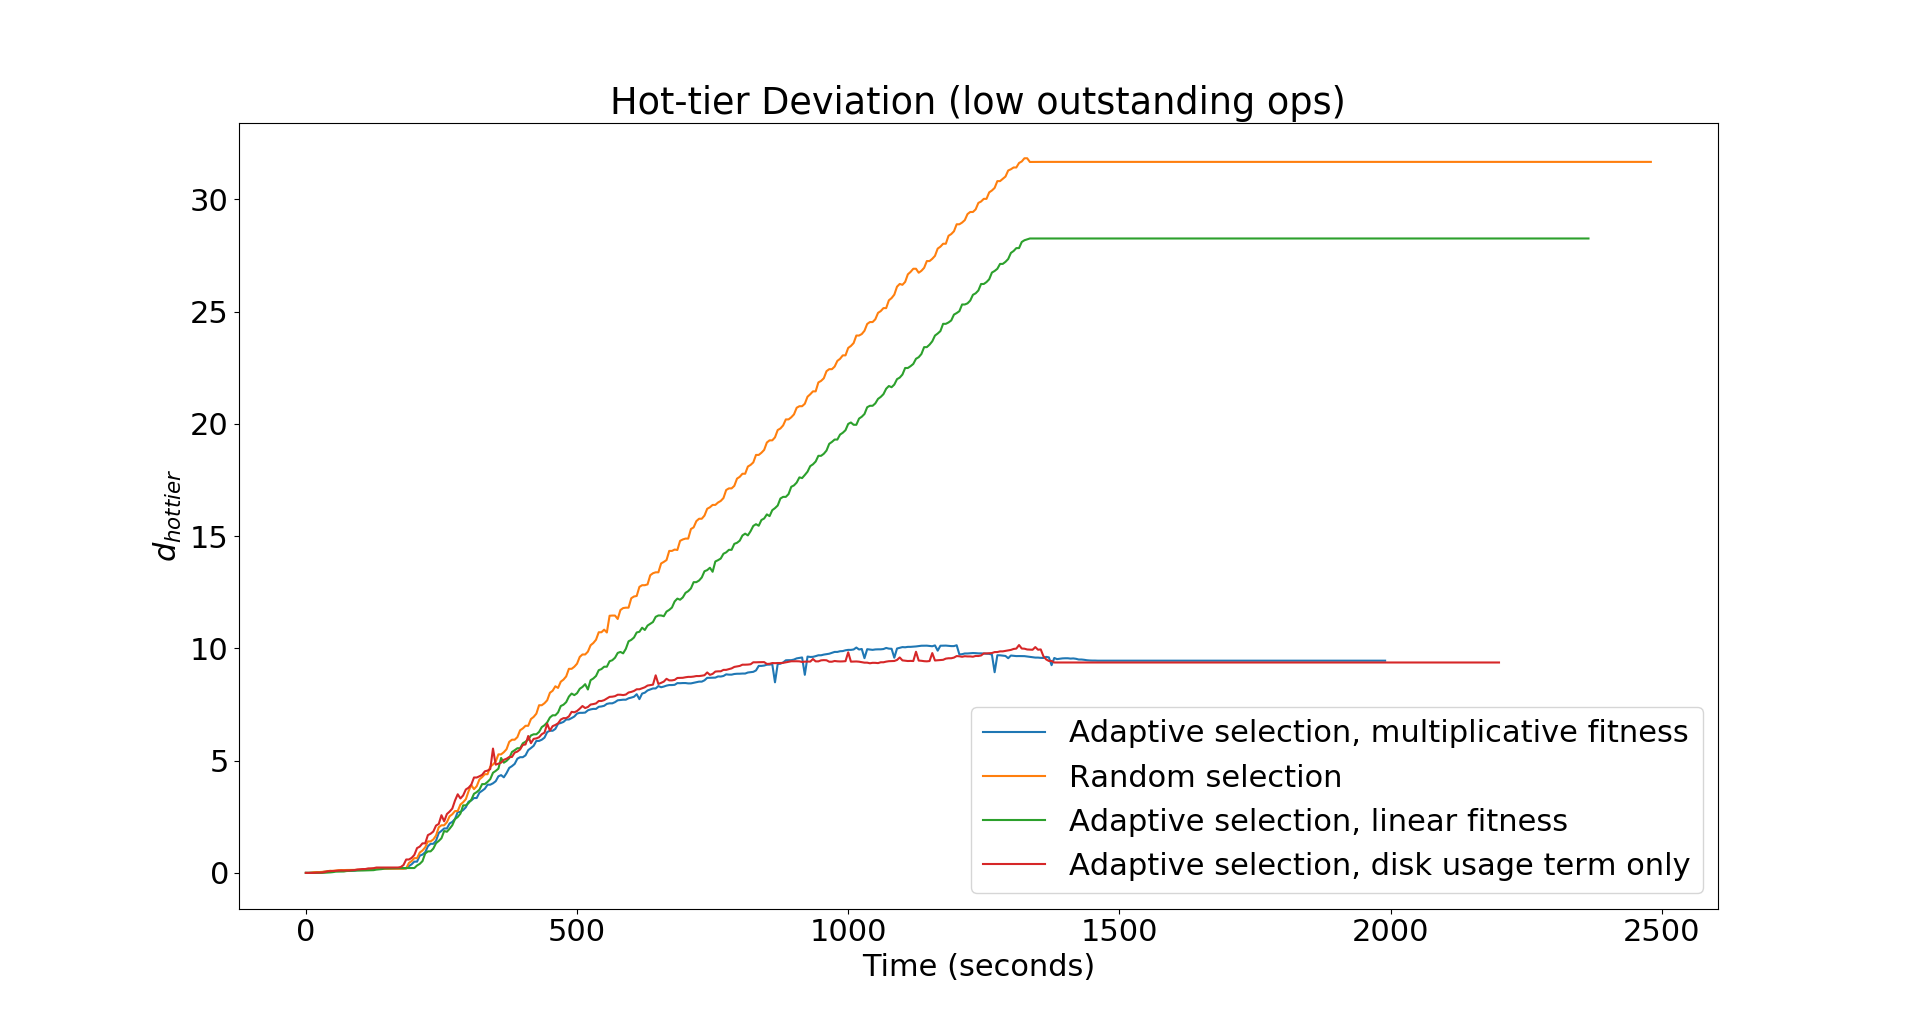
\includegraphics[scale=0.32]{images/low_outstanding_exp.png} 
      \caption{$d_{hot\ tier}$ values over time for low outstanding I/O
               operations.}
      \label{fig:low_outstanding_tier_disparity}
    \end{figure}

    Figure \ref{fig:low_outstanding_tier_disparity} shows the results of a
    workload with only a single outstanding operation. This causes the queue
    length reported by Stargate to be at most 1, resulting in the fitness
    function's queue length term to be roughly constant and approximately 1.
    
    \FloatBarrier

    It is evident that the additive fitness function does not minimize the
    hot-tier deviation as well as the multiplicative since the additive fitness
    function's behavior varies depending on the weight chosen for the queue
    length term. By default, the linear fitness function
    gives equal weight to both the disk fullness and queue length terms;
    however, for one run of this experiment the queue length term was given no
    weight. Linear fitness that gives equal weight to both terms does not
    reduce skew by very much, while giving no weight to the queue length term
    keeps all nodes' SSD usages within 10\% of each other. A linear fitness
    function does a poor job of reducing $d_{hot\ tier}$ values because the
    queue length term is contributing the maximum amount possible to the
    fitness value due to the consistently low queue length values. This can be
    illustrated by defining a disk selection bias, $b_r$, as the probability
    some disk, $d$, will be selected when compared with another disk, $d'$
    whose utilization is 10\% higher and queue length value is identical. Given
    a fitness function, $f$, $b_r$ can be calculated as follows:

    \begin{equation}
      b_r = \frac{f(d)}{f(d) + f(d')}
    \end{equation}

    Figures \ref{fig:bias_max_qlen} and \ref{fig:bias_min_qlen} show the disk
    selection biases for very large and very small queue lengths respectively.

    \begin{figure}[htbp]
      \centering
      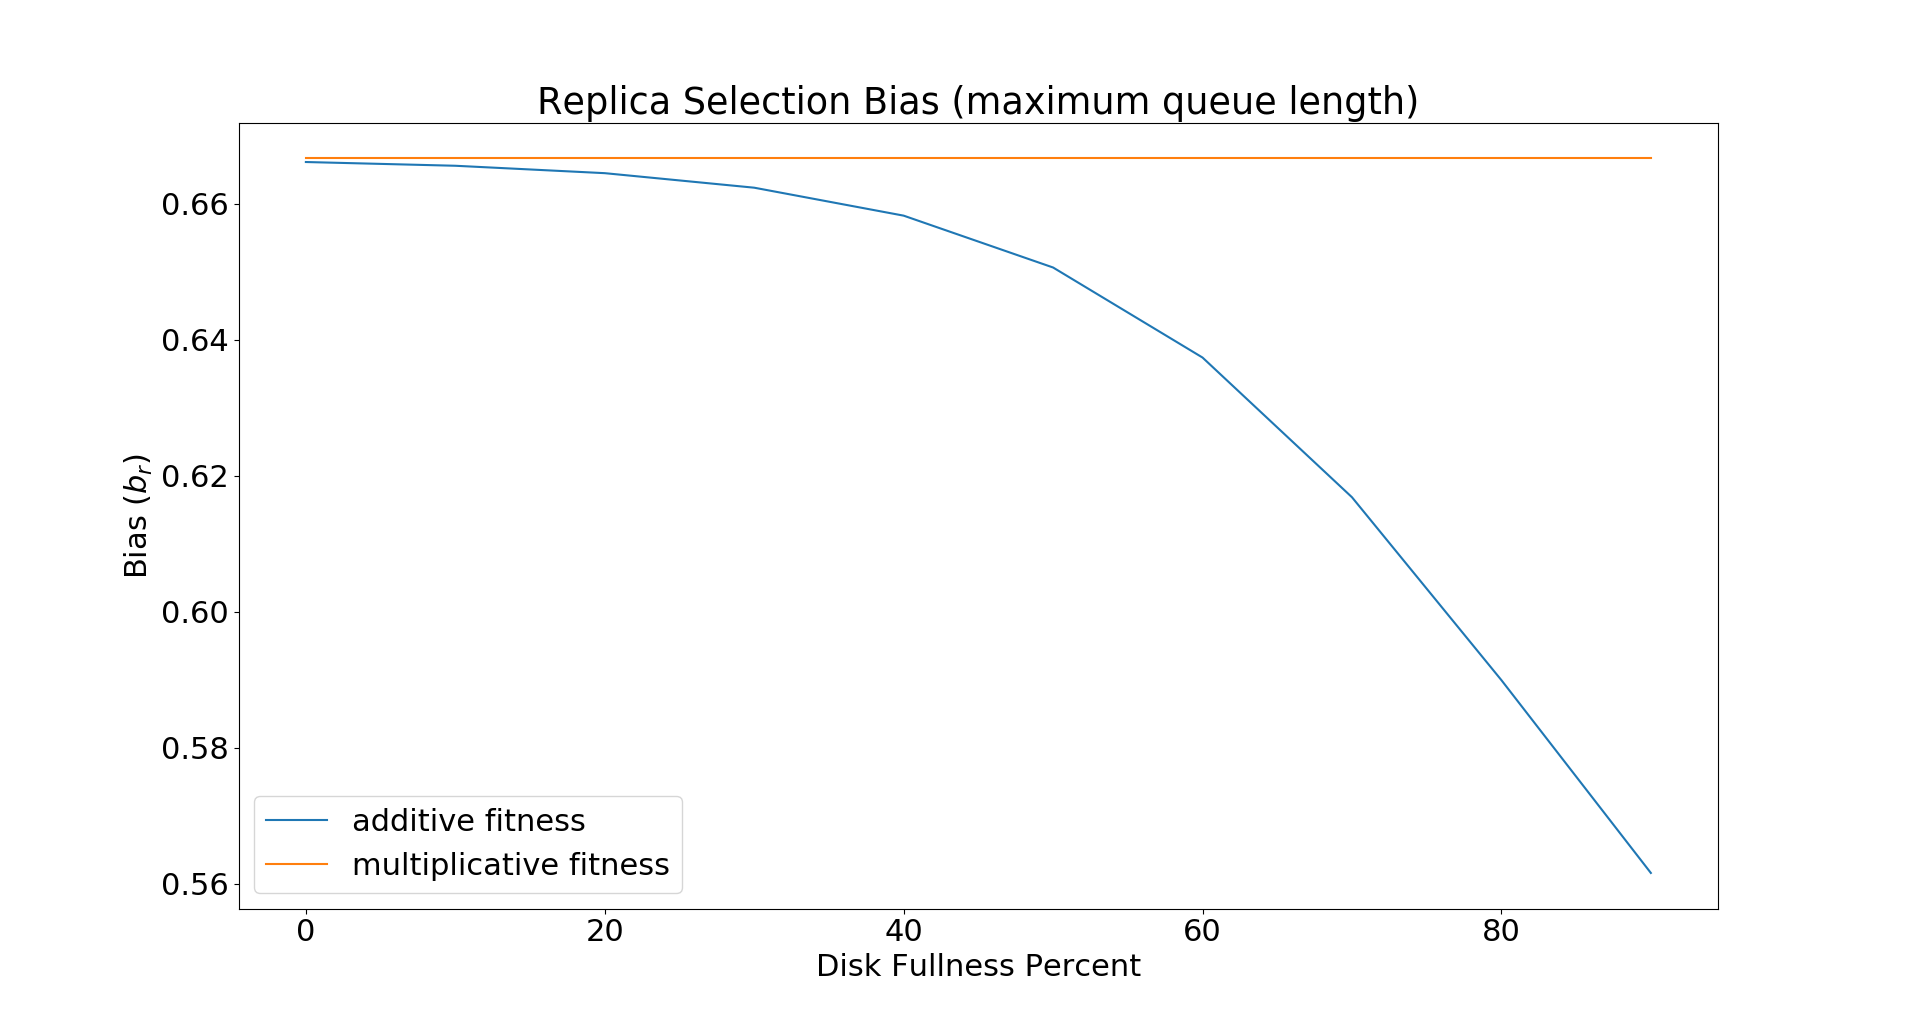
\includegraphics[scale=0.32]{images/replica_selection_bias_max_qlen.png} 
      \caption{$b_r$ values with static queue lengths at the fitness
               function ceiling values.}
      \label{fig:bias_max_qlen}
    \end{figure}

    \begin{figure}[htbp]
      \centering
      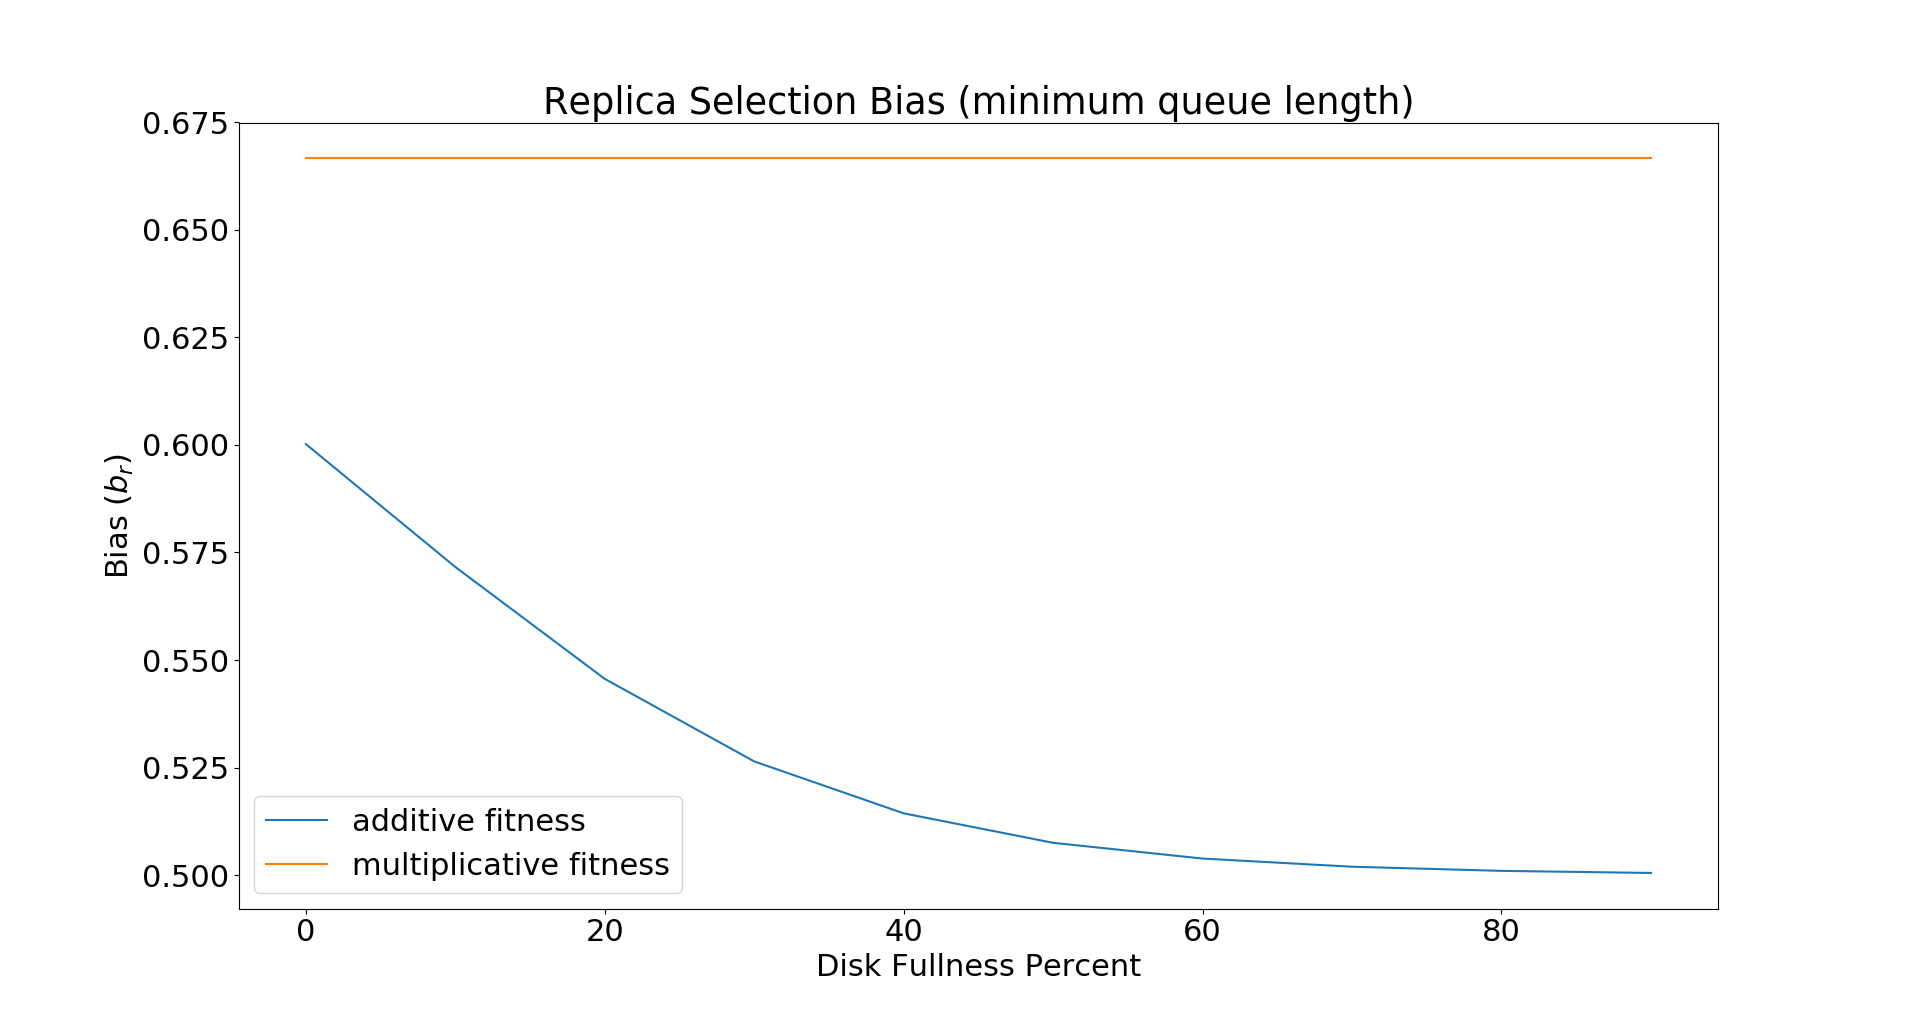
\includegraphics[scale=0.32]{images/replica_selection_bias_min_qlen.png} 
      \caption{$b_r$ values with static queue lengths at 1.}
      \label{fig:bias_min_qlen}
    \end{figure}

    For an additive fitness function, the bias towards a less utilized disk
    decreases as the disk fullness percentages for $d$ and $d'$ increase, even
    though they still only differ by 10\% in Figures \ref{fig:bias_max_qlen}
    and \ref{fig:bias_min_qlen}. The entire linear fitness function does not
    scale with each term, so the multiplicative fitness function is superior.

    \subsubsection{High Outstanding Operation Results}
    \label{sec:high-outstanding-ops}

    \begin{figure}[htbp]
      \centering
      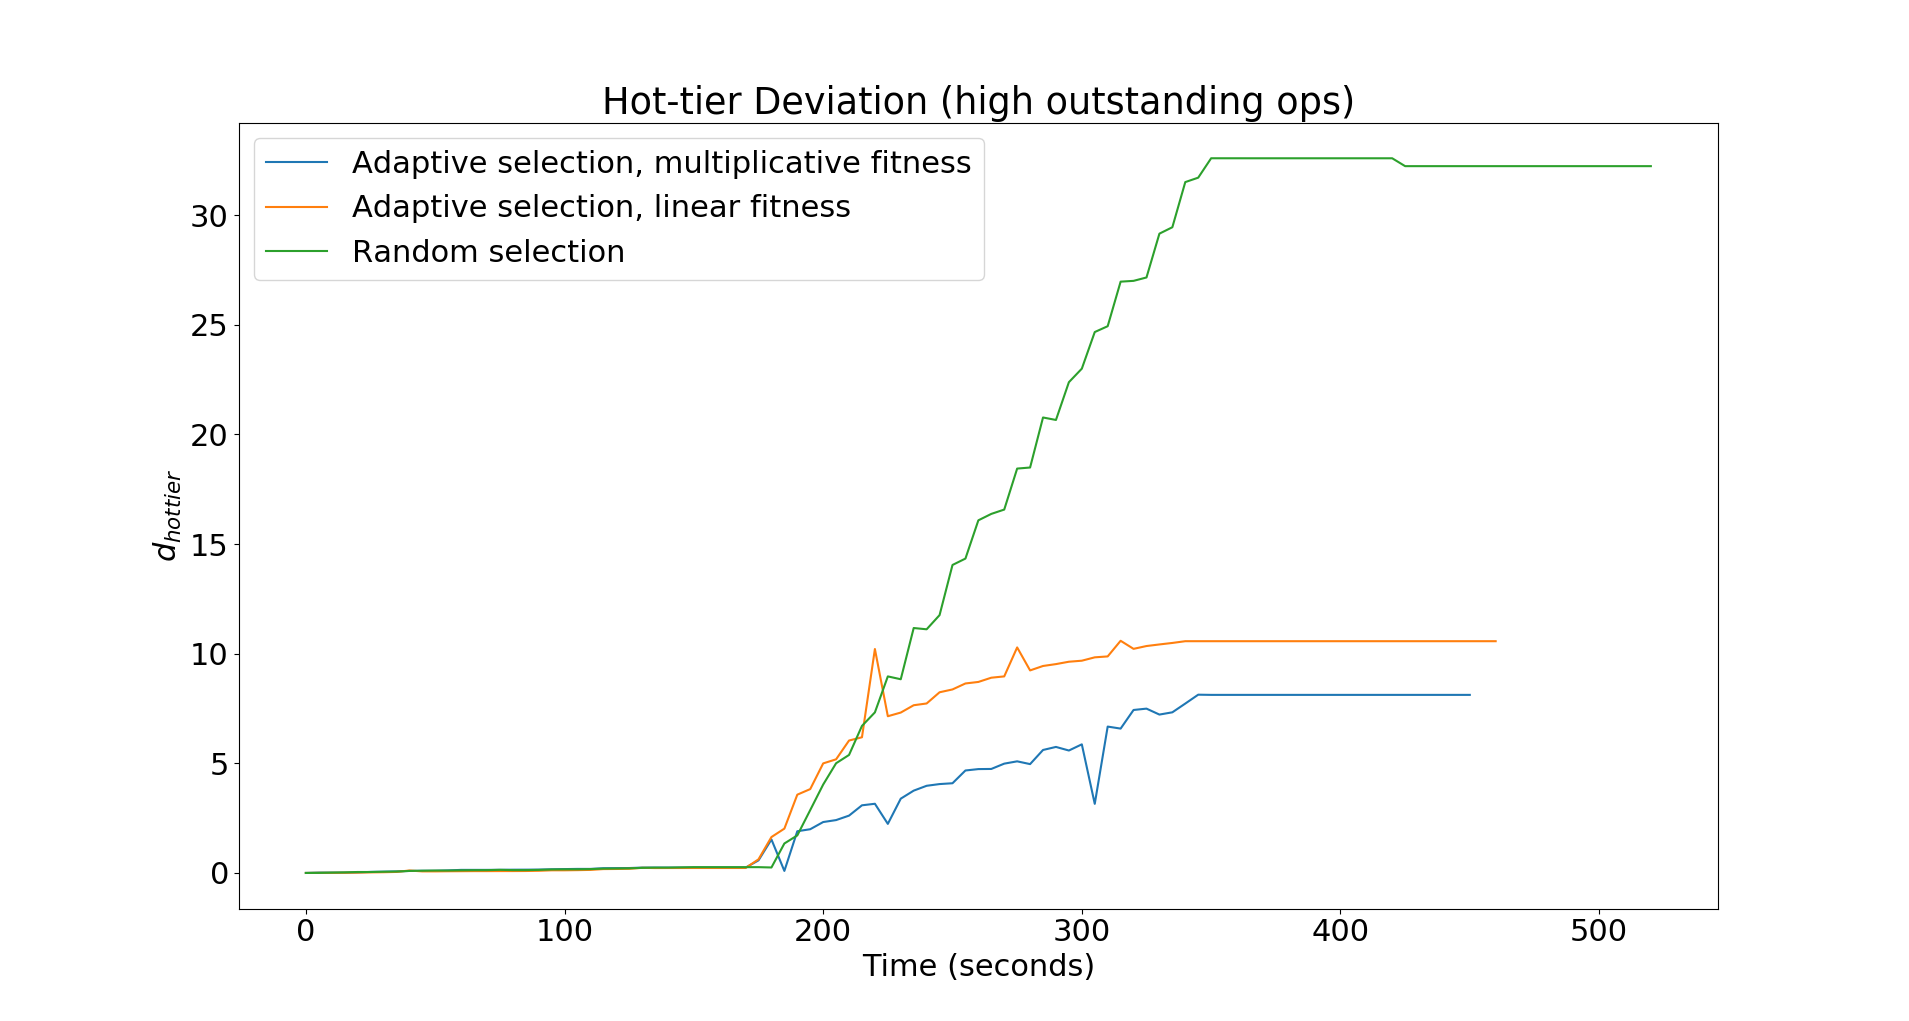
\includegraphics[scale=0.32]{images/high_outstanding_exp.png} 
      \caption{$d_{hot\ tier}$ values over time for low outstanding I/O
               operations.}
      \label{fig:high_outstanding_tier_disparity}
    \end{figure}


    Figure \ref{fig:high_outstanding_tier_disparity} shows that both additive
    and multiplicative fitness functions reduce the disk fullness skew from
    30\% to less than 10\%. Multiplicative fitness performs slightly better at
    minimizing $d_{hot\ tier}$ than additive fitness, possibly due to scaling
    the fitness value by the value of both the fullness and queue length terms,
    rather than weights.
  
  \subsection{Disk Queue Length Experiments} \label{experiments-qlen}

  Due to the nature of low outstanding I/O workloads, disk queue length values
  would remain very low for the duration of an experiment. This does not give
  useful information for measuring the effects of fitness-based replica
  selection on disk queue lengths. The experiments for high outstanding I/O
  experiments in section \ref{sec:high-outstanding-ops} was re-run for all
  fitness function types and for fitness function queue length term ceilings of
  200 and 100. Figures \ref{fig:qlen_100} and \ref{fig:qlen_200} show a
  reduction in queue length quartiles when fitness-based selection is used for
  disks on nodes that host local workloads. Lower queue length ceilings are
  observed to provide better results in reducing the queue lengths for the
  worker nodes.

  \begin{figure}[!htb]
    \centering
    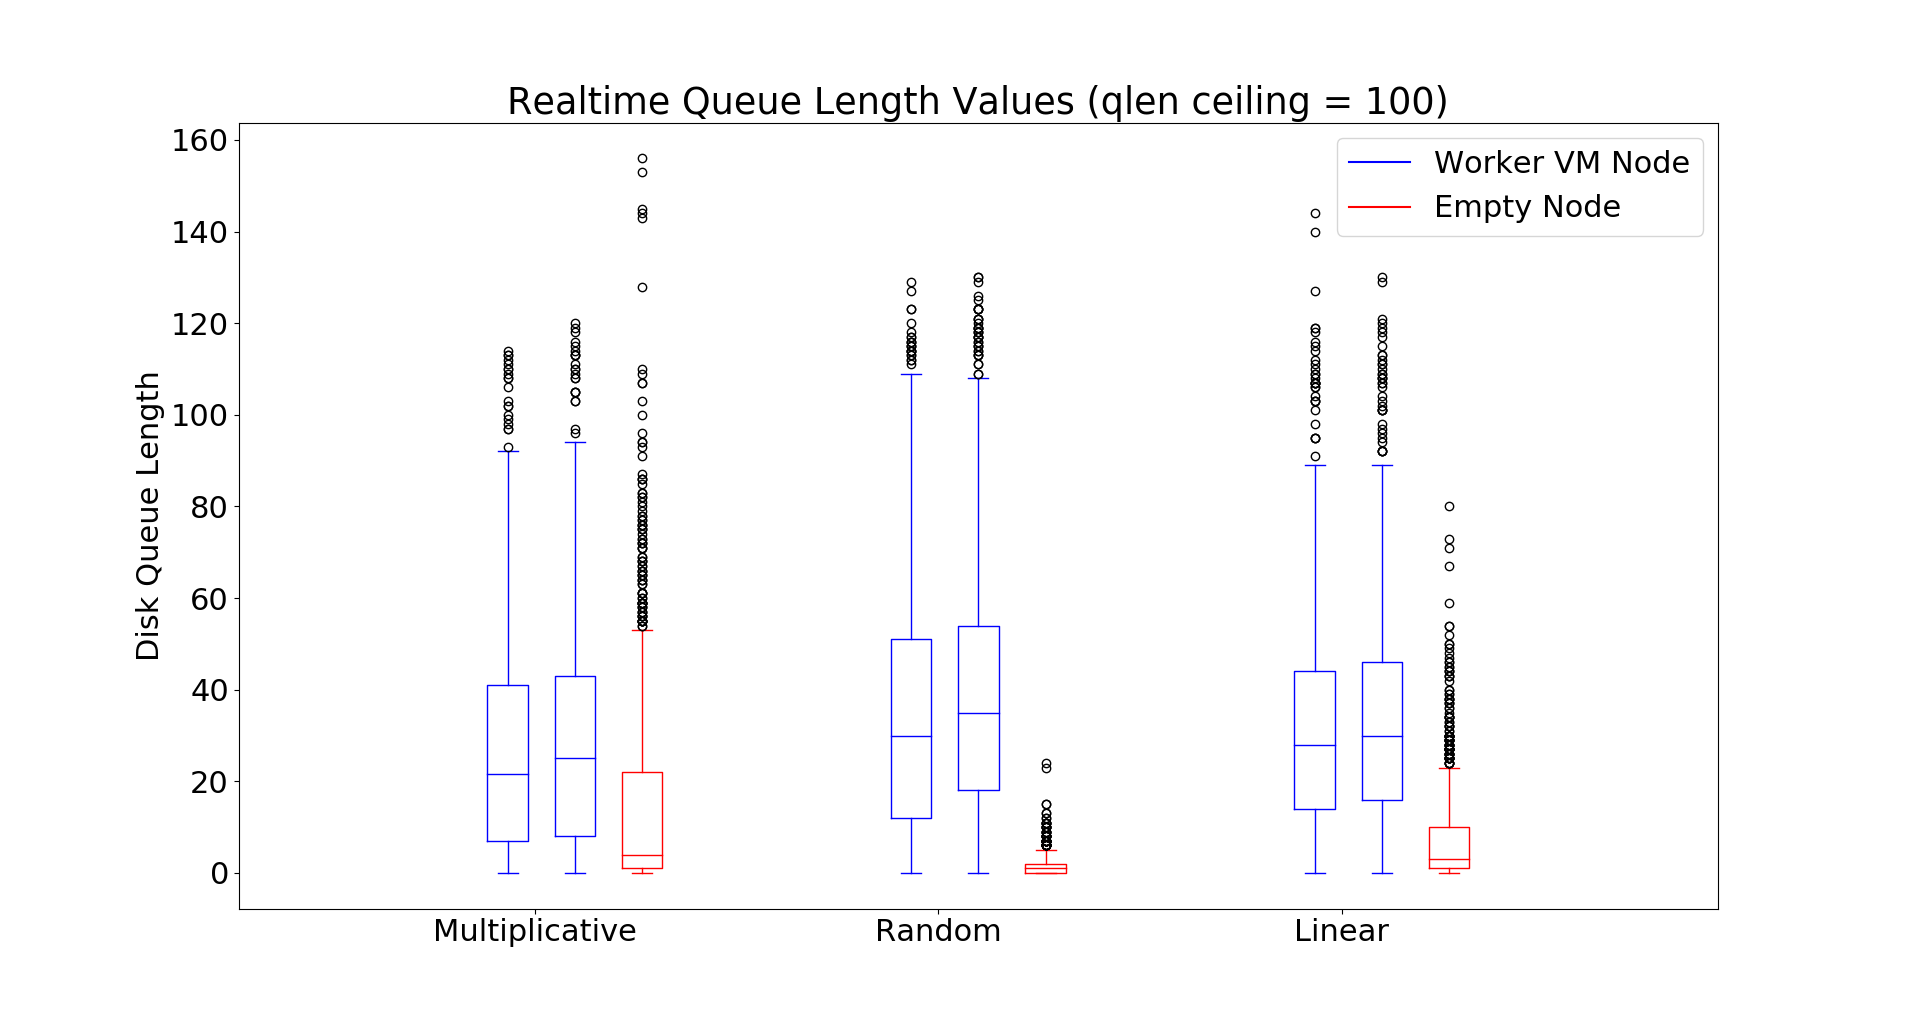
\includegraphics[scale=0.32]{images/qlen_100_box.png} 
    \caption{Queue lengths for all SSDs on the specified nodes sampled every 1
             second.}
    \label{fig:qlen_100}
  \end{figure}

  \begin{figure}[!htb]
    \centering
    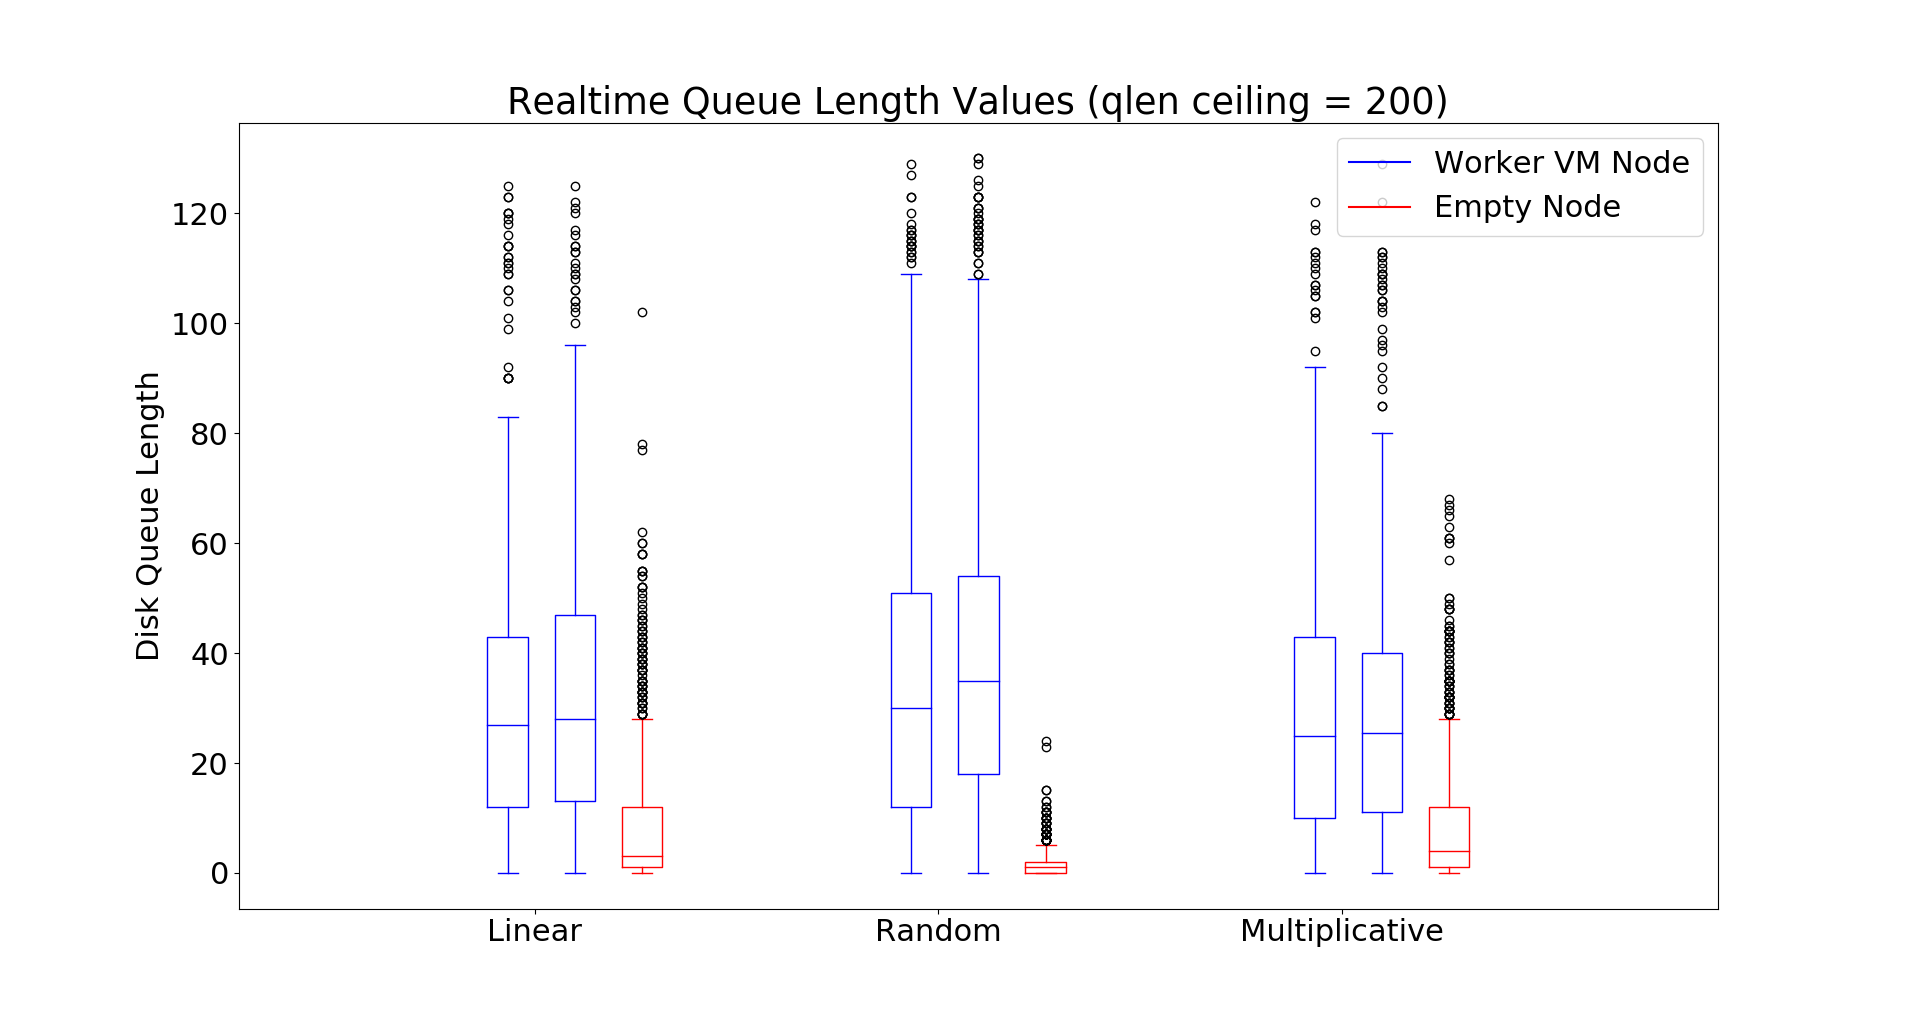
\includegraphics[scale=0.32]{images/qlen_200_box.png} 
    \caption{Queue lengths for all SSDs on the specified nodes sampled every 1
             second.}
    \label{fig:qlen_200}
  \end{figure}

%%%%%%%%%%%%%%%%%%%%%%%%%%%%%%%%%%%%%%%%%%%%%%%%%%%%%%%%%%%%%%%%%%%%%%%%%%%%%%%
\newpage
\FloatBarrier
\section{User Guide}

  \subsection{Scraping Data From the Nutanix Cluster}

  Stargate exposes a web server on the CVM, listening on port 2009, that
  exposes various real-time stats such as the number of operations in flight,
  disk throughput, disk queue length, and many other pieces of information. I
  wrote a Python script to parse and derive the following information for each
  node:

  \begin{tcolorbox}
  \begin{enumerate}
    \item SSD tier usage
    \item SSD tier availability
    \item SSD tier max capacity
    \item Read/Write counts for each disk
    \item Queue lengths for each disk
  \end{enumerate}
  \end{tcolorbox}

  The script will filter out all disks in the HDD tier and only pull the
  statistics for the SSD tier. Upon each invocation of the script, information
  is appended to a file for each node that is created if it is non-existent.
  The data is layed out in a CSV format for easy plotting via the Matplotlib
  library \cite{matplotlib}. For each experiment, the script was called every 5
  seconds via the command \texttt{watch -n 5}.

  \subsection{Re-creating Experiments}

  An NX-1350 with VMware ESXi 5.5u2 hypervisor and a single 300GB SSD on each
  node was used for all experiments. This means that for an RF2
  cluster, there is less than 150GB of useable hot tier available since a small
  amount of space is reserved on each disk for other services on the CVM.

  A single CentOS 6.5 worker VM was manually created on a single node with 4GB
  RAM, single 150GB disk, and installation of Fio. The VM was packaged as a
  file in Open Virtualization Format (OVF) for ease of deployment to the host
  hypervisor. This removed the need for a tool to use the VMware vSphere API to
  deploy the worker VMs as mentioned in the proposal for this thesis.

  The Worker VM's 150GB disk size ensures that the entire hot tier of each node
  will be fully utilized when the disk is filled via workload generation on
  each node. Each of the other nodes then clone the worker VM so that all nodes
  in the cluster have an identical worker VM, worker VM disk state, and Nutanix
  node tier utilization.

  The Fio script used to generate a sequential write workload on each node is
  as follows:
  
  \singlespace
  \begin{tcolorbox}
  \begin{verbatim}
    [global]
    direct=1
    ioengine=libaio
    bs=32k
    iodepth=128
    randrepeat=0
    group_reporting
    filesize=150G

    [job1]
    rw=write
    filename=/dev/sdb
    name=sequential-write
  \end{verbatim}
  \end{tcolorbox}
  \doublespace

  The \texttt{iodepth} variable is modified depending on the number of
  outstanding I/Os needed.

  When resetting the cluster for a new test, the commands \texttt{cluster stop
  ; cluster destroy} were run on the CVM and the old Stargate binary was
  swapped with the one required for the next tests in the
  \texttt{/home/nutanix/bin/} directory.  When ready, it's necessary to
  recreate the Nutanix cluster via \texttt{cluster -s <cvm IPs> create} and
  deploy new worker VMs. The process is then repeated for each different test.

%%%%%%%%%%%%%%%%%%%%%%%%%%%%%%%%%%%%%%%%%%%%%%%%%%%%%%%%%%%%%%%%%%%%%%%%%%%%%%%
\newpage
\FloatBarrier
\section{Summary and Conclusions}

  Prior to this work, the problem of selecting a location for the placement of
  data replicas in a Nutanix cluster was solved by choosing disks in a uniform
  random fashion. This method of data placement does not perform well in the
  presence of heterogeneous workloads or tier size disparities. This work has
  shown that candidate disks for data placement can be evaluated using a
  function of observed queue length and fullness percentage values. The result
  of this function, the fitness value, can be used to bias disk selections towards
  disks that are less busy and less full. Biasing disk selections results in
  an overall even utilization of individual disk space and shows potential for
  a reduction of disk queue lengths for disks residing on busy nodes.

  \subsection{Limitations}

  The current weighted random selection approach, Stochastic Universal
  Sampling, is optimized for clusters that do not contain extremely large
  numbers of disks. While SUS allows disk selection probabilities to scale
  proportional to the fitness values of the disks, it is not as scalable as the
  two-choice method for weighted random selection.

  In addition, each Stargate's freqency of stats updates will impact its view
  of the world and can lead to herding behaviors if updates are not frequent
  enough. In the absence of a Stargate's ability to update its view of the
  world, it will be unable to adapt to changes in workload characteristics or
  disk fullness, which defeats the purpose of using fitness-based disk
  selections in the first place.

  \subsection{Future Work}

    \subsubsection{Real-time Fitness Feedback}

    The replica placement scheme shown in this work relies on periodic stats
    updates, therefore the system is always working with older stats for data placement
    decisions. One change that can be made to this system is to track the time to
    completion of various operations that place data on each disk and bias the replica
    placements towards the faster disks. This would remove the dependence on a centralized
    stats repository such as Arithmos and allow each Stargate to make data
    placement decisions independent of reports from other nodes in the cluser.
    Stargate would be required to keep a history latency data for each
    operation on remote nodes.

    \subsubsection{Read Replica Selection}

    When choosing which replicas to read from, Stargate always selects local
    disks. However, if there were ever a scenario where a read from a remote
    disk containing the desired data is faster than servicing the read from a
    local disk, Stargate is not currently equipped to detect or act on this
    scenario. Currently, disk fitnes values are not factored into the selection
    of disks that will service a read operation. More work will be required to
    add support for fitness-based read replica selection.
    
    \subsubsection{More Fitness Function Variables}

    The disk fitness values do not need to be limited to derivation from disk
    queue length and fullness percentage. The cluster tracks many other variables
    such as average node CPU utilization, number of Stargate failures in a
    specified time window, number of active hosted VMs, and data access patterns
    among other pieces of information. More investigation should occur to see how
    this data can be used to make better data placement decisions.

%%%%%%%%%%%%%%%%%%%%%%%%%%%%%%%%%%%%%%%%%%%%%%%%%%%%%%%%%%%%%%%%%%%%%%%%%%%%%%%
% GLOSSARY

\newpage
\section*{Glossary}
\thispagestyle{empty}

\begin{tabular}{l}
\texttt{CVM} \\
Nutanix Controller Virtual Machine. \\

\texttt{Data Deduplication} \\
A data compression technique for removing multiple copies of the same data.

\texttt{Fitness Value}\\
A value representing the desirability of a disk for data placement.\\

\texttt{HDD} \\
Hard Disk Drive. \\

\texttt{Hypervisor} \\
Software that runs virtual machines. \\

\texttt{iSCSI} \\
An IP based storage networking standard.\\

\texttt{NFS} \\
A distributed file system protocol. \\

\texttt{OVF} \\
A standard for packaging software to run in virtual machines.\\

\texttt{Secondary Replica} \\
Refers to any replica of data written after the first copy. \\

\texttt{SSD} \\
Solid State Drive. \\

\texttt{vDisk} \\
A file abstraction in the Nutanix distributed file system. \\

\end{tabular}
\FloatBarrier

%%%%%%%%%%%%%%%%%%%%%%%%%%%%%%%%%%%%%%%%%%%%%%%%%%%%%%%%%%%%%%%%%%%%%%%%%%%%%%%
\newpage
\FloatBarrier
 \begin{thebibliography}{99}

  \bibitem{eigrp} Albrightson, R., Garcia-Luna-Aceves, J. J., and Boyle, J.  (1994). EIGRP--A fast routing protocol based on distance vectors. Interop 94.
  \bibitem{baker1987} Baker, J. E. (1987, July). Reducing bias and inefficiency in the selection algorithm. In Proceedings of the second international conference on genetic algorithms (pp. 14-21).
  \bibitem{hdfs2008} Borthakur, D. (2008). HDFS architecture guide. HADOOP APACHE PROJECT http://hadoop. apache. org/common/docs/current/hdfs design. pdf, 39.
  \bibitem{chao1982} Chao, M. T. (1982). A general purpose unequal probability sampling plan.  Biometrika, 69(3), 653-656.
  \bibitem{esxi2008} Chaubal, C. (2008). The architecture of vmware esxi. VMware White Paper, 1(7).
  \bibitem{raid2} Chen, P. M., Lee, E. K., Gibson, G. A., Katz, R. H., and Patterson, D. A. (1994). RAID: High-performance, reliable secondary storage. ACM Computing Surveys (CSUR), 26(2), 145-185.
  \bibitem{truncation1973} Crow, J. F., and Kimura, M. (1979). Efficiency of truncation selection. Proceedings of the National Academy of Sciences of the United States of America, 76(1), 396–399.
  \bibitem{mapreduce} Dean, J., and Ghemawat, S. (2008). MapReduce: simplified data processing on large clusters. Communications of the ACM, 51(1), 107-113.
  \bibitem{reservoir2006} Efraimidis, P. S., and Spirakis, P. G. (2006). Weighted random sampling with a reservoir. Information Processing Letters, 97(5), 181-185.
  \bibitem{gfs} Ghemawat, S., Gobioff, H., and Leung, S. T. (2003, October). The Google file system. In ACM SIGOPS operating systems review (Vol. 37, No.  5, pp. 29-43). ACM.
  \bibitem{hadoop} Hadoop, A. (2009). Hadoop. 2009-03-06].  \url{http://hadoop.apache.org}.
  \bibitem{matplotlib} Hunter, J. D. (2007). Matplotlib: A 2D graphics environment. Computing In Science and Engineering, 9(3), 90-95.
  \bibitem{adapt2012} Jin, H., Yang, X., Sun, X. H., and Raicu, I. (2012, June). Adapt: Availability-aware mapreduce data placement for non-dedicated distributed computing. In Distributed Computing Systems (ICDCS), 2012 IEEE 32nd International Conference on (pp. 516-525). IEEE.
  \bibitem{cassandra} Lakshman, A., and Malik, P. (2008, August 25). Cassandra – A structured storage system on a P2P Network. Retrieved February 15, 2016, from \url{https://www.facebook.com/notes/facebook-engineering/cassandra-a-structured-storage-system-on-a-p2p-network/24413138919/}
  \bibitem{paxos2005} Lamport, L. (2005). Generalized consensus and Paxos. Technical Report MSR-TR-2005-33, Microsoft Research.s
  \bibitem{distance-vector-1} McQuillan, J. M., Richer, I., Rosen, E. C., and Bertsekas, D. P. (1978). Arpanet routing algorithm improvements (No. BBN-3940). BOLT BERANEK AND NEWMAN INC CAMBRIDGE MA.
  \bibitem{2choice} Mitzenmacher, M. (2001). The power of two choices in randomized load balancing. IEEE Transactions on Parallel and Distributed Systems, 12(10), 1094-1104.
  \bibitem{raid} Patterson, D. A., Gibson, G., and Katz, R. H. (1988). A case for redundant arrays of inexpensive disks (RAID) (Vol. 17, No. 3, pp.  109-116). ACM.
  \bibitem{perez2003} Perez, J. M., Garcia, F., Carretero, J., Calderon, A., and Sanchez, L. M. (2003, May). Data allocation and load balancing for heterogeneous cluster storage systems. In Cluster Computing and the Grid, 2003. Proceedings. CCGrid 2003. 3rd IEEE/ACM International Symposium on (pp. 718-723). IEEE.
  \bibitem{stl} Plauger, P. J., Lee, M., Musser, D., and Stepanov, A. A. (2000). C++ Standard Template Library. Prentice Hall PTR.
  \bibitem{bible} Poitras, S. (n.d.) The Nutanix Bible. Retrieved August 09, 2017, from \url{http://www.nutanixbible.com/}
  \bibitem{igrp} Rutgers, C. L. H. (1991). “An introduction to igrp. The State University of New Jersey, Center for Computers and Information Services, Laboratory for Computer Science Research.
  \bibitem{breeder1993} Schlierkamp-Voosen, D., and Mühlenbein, H. (1993). Predictive models for the breeder genetic algorithm. Evolutionary Computation, 1(1), 25-49.
  \bibitem{suresh2015} Suresh, L., Canini, M., Schmid, S., and Feldmann, A. (2015). C3: Cutting tail latency in cloud data stores via adaptive replica selection. In 12th USENIX Symposium on Networked Systems Design and Implementation (NSDI 15) (pp. 513-527).
  \bibitem{python} Van Rossum, G., and Drake, F. L. (2003). Python language reference manual (p. 144). Network Theory.
  \bibitem{hyperv2009} Velte, A., and Velte, T. (2009). Microsoft virtualization with Hyper-V. McGraw-Hill, Inc..
  \bibitem{vitter1985} Vitter, J. S. (1985). Random sampling with a reservoir. ACM Transactions on Mathematical Software (TOMS), 11(1), 37-57.
  \bibitem{xie2010} Xie, J., Yin, S., Ruan, X., Ding, Z., Tian, Y., Majors, J., ... and Qin, X. (2010, April). Improving mapreduce performance through data placement in heterogeneous hadoop clusters. In Parallel and Distributed Processing, Workshops and Phd Forum (IPDPSW), 2010 IEEE International Symposium on (pp. 1-9). IEEE.
  \bibitem{azar1994} Y. Azar, A. Broder, A. Karlin, and E. Upfal. Balanced allocations. In Proceedings of the 26th ACM Symposium on the Theory of Computing, pages 593\{602, 1994.
  \bibitem{zaharia2008} Zaharia, M., Konwinski, A., Joseph, A. D., Katz, R.  H., and Stoica, I. (2008, December). Improving MapReduce Performance in Heterogeneous Environments. In OSDI (Vol. 8, No. 4, p. 7).


 \end{thebibliography}

%%%%%%%%%%%%%%%%%%%%%%%%%%%%%%%%%%%%%%%%%%%%%%%%%%%%%%%%%%%%%%%%%%%%%%%%%%%%%%%
\newpage
\FloatBarrier
\begin{appendices}
\appendix
\section{Appendix}

  \subsection{Herding Behavior Due to Implementation Bug}

  During the 128 outstanding op experiments, herding behavior
  was observed unexpectedly after implementing fitness based replica placement
  as shown in Figure \ref{fig:herding_bug}. By default, disk usage and
  performance stats are supposed to be refreshed every 10 seconds. This is
  frequent enough to avoid herding behavior, but the 128 outstanding op
  experiments exhibited herding.

  \begin{figure}[htbp]
    \centering
    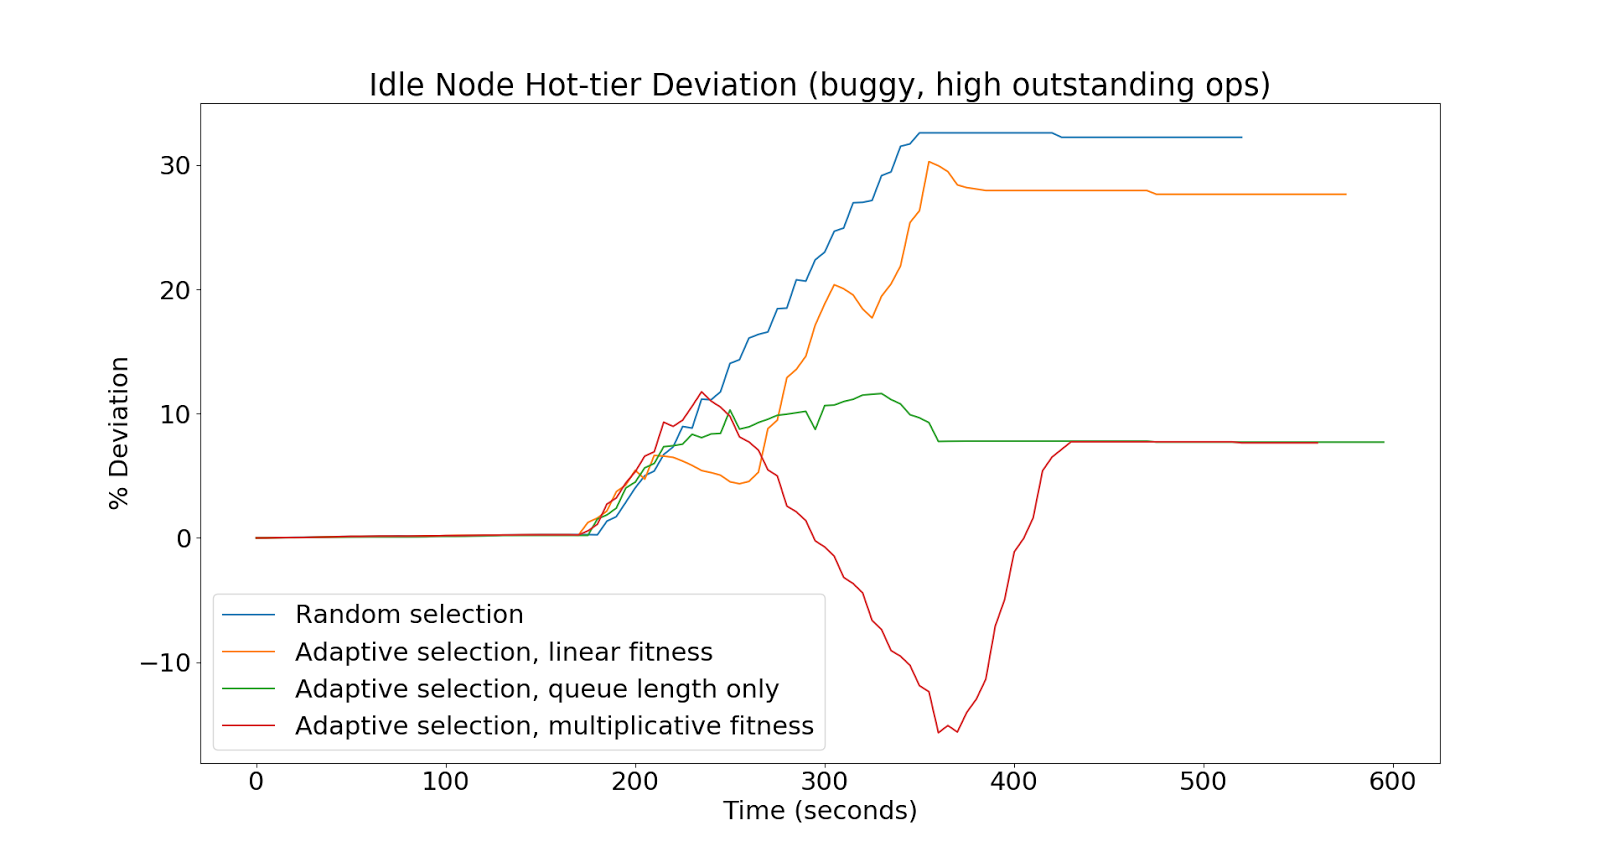
\includegraphics[scale=0.30]{images/buggy.png} 
    \caption{$d_{hot\ tier}$ values over time for low outstanding I/O
             operations. This set of experiments contains the stats update bug.}
    \label{fig:herding_bug}
  \end{figure}

  The experiment with additive fitness seemed to only exhibit mild herding
  behavior, whereas the test with multiplicative fitness showcased much more
  dramatic shifts in SSD usage skews. In conjunction with the complete absence
  of this behavior in the single outstanding op experiments, it was thought to
  be highly likely that this herding behavior was caused by a bug in the queue
  length term of the fitness functions. An additive fitness function is less
  affected by this bug due to the attenuated effect of each term in the fitness
  function.

  Within Stargate, a mapping is kept from disk ID to a DiskState object (called
  \texttt{disk\_map\_}) containing information and cached statistics related to
  the disk. The disk performance and disk usage stats are two separate elements
  within the DiskState structure.

  Every 10 seconds, an alarm handler will execute and iterate through each
  active disk in the cluster and asynchronously query disk stats and bind a
  callback to each query to be executed when a response is received. Disk usage
  and performance lookups each have their own callback functions:

  \begin{table}[htbp]
    \caption{Disk usage and performance lookup callback functions.}
    \begin{center}
    \begin{tabular}{ | p{0.5\linewidth} | p{0.5\linewidth} | }
      \hline
      \textbf{Function Name} & \textbf{Description} \\ \hline
      \verb|UsageStatLookupCallback| & Decrement the outstanding stats lookup
                                       counter, acquire lock and populate
                                       performance stats in
                                       \texttt{disk\_map\_}, and leave
                                       performance stats untouched.
                                       \\ \hline

      \verb|PerformanceStatLookupCallback| & Decrement outstanding stats
                                             lookup counter, lock and
                                             populate performance stats in
                                             \texttt{disk\_map\_}, and leave
                                             usage stats untouched. \\ \hline

      \hline
    \end{tabular}
    \end{center}
  \end{table}

  The two callbacks introduce a race condition regarding \texttt{disk\_map\_}
  even though the structure is locked. Any time PerformanceStatLookupCallback
  returns before the callback for usage stats, all performance stats will be
  cleared and cause the fitness function to assume worst-case values for the
  queue length term.

  This problem was fixed by simply serializing our usage and performance stats
  lookups.

\end{appendices}

\end{document}
